%======================================================================
%  CSE 450 Capstone Project -- Report
%  Department of Computer Science and Engineering, BUET
%======================================================================
\documentclass[10pt,a4paper,oneside]{report}
\usepackage{cse-capstone}

% ---- Project-specific packages and macros ----------------------------
\usepackage{tikz}
\usepackage{pgfplots}
\pgfplotsset{compat=1.17}
\usepackage{colortbl}
%======================================================================
%  Shared palette and TikZ styles for every architecture / pipeline figure.
%  Loaded once from template.tex (and from the standalone preview harness).
%======================================================================
\usetikzlibrary{arrows.meta,positioning,fit,backgrounds,calc,
  shapes.geometric,shapes.misc,decorations.pathreplacing,decorations.markings}

% ---- Palette: one hue per functional role, used in every figure -----
% Persuader / merchant stream
\definecolor{PerMain}{HTML}{E11D48}\definecolor{PerFill}{HTML}{FFE4E6}\definecolor{PerBord}{HTML}{BE123C}
% Persuadee / buyer / decider stream
\definecolor{DecMain}{HTML}{2563EB}\definecolor{DecFill}{HTML}{DBEAFE}\definecolor{DecBord}{HTML}{1D4ED8}
% Directional cross-attention
\definecolor{XatMain}{HTML}{7C3AED}\definecolor{XatFill}{HTML}{EDE9FE}\definecolor{XatBord}{HTML}{6D28D9}
% Trajectory GRU and attention pooling
\definecolor{TrjMain}{HTML}{059669}\definecolor{TrjFill}{HTML}{D1FAE5}\definecolor{TrjBord}{HTML}{047857}
% Outputs and fusion heads
\definecolor{Slate}{HTML}{0F172A}\definecolor{SlateSoft}{HTML}{475569}
% Neutral encoders and data
\definecolor{NeuFill}{HTML}{F1F5F9}\definecolor{NeuBord}{HTML}{64748B}
% Accent for the strategy stream and warnings
\definecolor{AmbFill}{HTML}{FEF3C7}\definecolor{AmbBord}{HTML}{B45309}\definecolor{AmbMain}{HTML}{D97706}

\tikzset{
  every picture/.append style={font=\footnotesize, >=Stealth,
    execute at begin picture={\hyphenpenalty=10000\relax\exhyphenpenalty=10000\relax}},
  blk/.style={rectangle, rounded corners=3pt, line width=0.8pt, align=center,
              inner xsep=4pt, inner ysep=3pt, minimum height=0.62cm},
  per/.style={blk, draw=PerBord, fill=PerFill},
  dec/.style={blk, draw=DecBord, fill=DecFill},
  xat/.style={blk, draw=XatBord, fill=XatFill},
  trj/.style={blk, draw=TrjBord, fill=TrjFill},
  neu/.style={blk, draw=NeuBord, fill=NeuFill},
  amb/.style={blk, draw=AmbBord, fill=AmbFill},
  fin/.style={blk, draw=Slate, fill=Slate, text=white},
  ten/.style={rectangle, rounded corners=1.5pt, draw=NeuBord, fill=white,
              line width=0.5pt, inner sep=1.6pt, font=\scriptsize},
  nt/.style={font=\scriptsize\itshape, text=SlateSoft, align=center},
  flow/.style={-{Stealth[length=4.2pt,width=3.6pt]}, line width=0.9pt, draw=SlateSoft},
  flowP/.style={-{Stealth[length=4.2pt,width=3.6pt]}, line width=1.0pt, draw=PerMain},
  flowD/.style={-{Stealth[length=4.2pt,width=3.6pt]}, line width=1.0pt, draw=DecMain},
  flowX/.style={-{Stealth[length=4.2pt,width=3.6pt]}, line width=1.0pt, draw=XatMain},
  flowT/.style={-{Stealth[length=4.2pt,width=3.6pt]}, line width=1.0pt, draw=TrjMain},
  dsh/.style={dashed, dash pattern=on 3pt off 2pt},
  grp/.style={rectangle, rounded corners=6pt, line width=0.7pt, draw=#1, fill=#1!6,
              inner sep=6pt},
  ttl/.style={font=\footnotesize\bfseries, align=center},
  oplus/.style={circle, draw=Slate, fill=white, line width=0.8pt, inner sep=0pt,
                minimum size=0.42cm, font=\footnotesize},
}

\usepackage[htt]{hyphenat}
\renewcommand{\_}{\textunderscore\penalty0\relax}
\setlength{\emergencystretch}{2.5em}


% Unconfirmed administrative/external information macro (Section 1.C)
\newcommand{\pending}[1]{\textcolor{red}{[PENDING: #1]}}

% ---------------------------------------------------------------------
\newcommand{\ProjectTitle}{Antiphony}
\newcommand{\ProjectSubtitle}{Dual-Perspective Modeling of Persuasion and Commitment in Asymmetric Dialogue}
\newcommand{\TeamName}{Group 10}
\newcommand{\Session}{Session 2026--2027}
\newcommand{\SubmissionDate}{September 2026}
\newcommand{\SupervisorName}{Dr. Md. Shariful Islam Bhuyan}
\newcommand{\SupervisorDesignation}{Associate Professor, Department of CSE, BUET}
\newcommand{\Supervisors}{\SupervisorName, \SupervisorDesignation}
% Team members are listed in frontmatter/titlepage.tex and declaration.tex
% ---------------------------------------------------------------------

\hypersetup{pdftitle={\ProjectTitle: \ProjectSubtitle}}

\begin{document}

\pagenumbering{gobble}
\thispagestyle{empty}

\begin{center}
    % Institution crest and department
    \includegraphics[width=28mm]{buet_logo.png}\\[8pt]
    {\large\textbf{Department of Computer Science and Engineering}}\\[2pt]
    {\large\textbf{Bangladesh University of Engineering and Technology}}\\[2pt]
    Dhaka, Bangladesh

    \vspace*{1.6cm}

    {\color{darkslate!85}\normalsize\scshape CSE 450 Capstone Project Final Report}

    \vspace*{0.8cm}

    % Title and subtitle
    {\color{secondary}\rule{0.55\textwidth}{1pt}}\\[14pt]
    {\fontsize{36pt}{40pt}\selectfont\bfseries\color{primary} \ProjectTitle}\\[12pt]
    \parbox{0.72\textwidth}{\centering\Large\color{darkslate} \ProjectSubtitle}\\[10pt]
    {\color{secondary}\rule{0.55\textwidth}{1pt}}

    \vspace*{1.6cm}

    % Team
    {\large\bfseries\color{secondary} Submitted by \TeamName}\\[8pt]
    {\normalsize\renewcommand{\arraystretch}{1.25}
    \begin{tabular}{@{}l l@{}}
        Arnob Biswas         & 2105015 \\
        Nawriz Ahmed Turjo   & 2105032 \\
        Abhishek Roy         & 2105033 \\
        Monjur Hossain Khan  & 2105043 \\
        Shams Hossain Simanto & 2105048 \\
    \end{tabular}}

    \vspace*{1.2cm}

    % Supervisor
    {\large\bfseries\color{secondary} Supervised by}\\[8pt]
    {\normalsize\textbf{\SupervisorName}}\\[2pt]
    {\normalsize\SupervisorDesignation}

    \vfill

    {\normalsize \Session \quad\textbullet\quad \SubmissionDate}
\end{center}

\clearpage

\pagenumbering{roman}
\begin{center}
  {\Large\bfseries CANDIDATES' DECLARATION}
\end{center}
\addcontentsline{toc}{chapter}{Candidates' Declaration}

\vspace{20pt}
We declare that the work presented in this report, titled
``\ProjectTitle: \ProjectSubtitle'', is the outcome of the engineering and research work carried out by us
under the supervision of \SupervisorName, \SupervisorDesignation.

All prior work, third-party code, libraries, data, copyrighted material, and
tools used in the project have been properly acknowledged. Any use of
generative AI tools has been disclosed in accordance with academic integrity guidelines. We accept accountability and
responsibility for the accuracy and integrity of this report and for our
individual contributions to the project.

\newcommand{\signature}[2][13mm]{\includegraphics[height=#1,width=0.4\textwidth,keepaspectratio]{sign/clean/#2}}
\vspace{10mm}
\begin{tabular}{>{\raggedright\arraybackslash}p{0.45\textwidth} >{\raggedright\arraybackslash}p{0.45\textwidth}}
  \signature[18mm]{arnob} & \signature{turjo} \\[-2mm]
  \rule{0.4\textwidth}{0.4pt} & \rule{0.4\textwidth}{0.4pt} \\
  Arnob Biswas (2105015) & Nawriz Ahmed Turjo (2105032) \\[10mm]
  \signature[17mm]{abhishek} & \signature{shovon} \\[-2mm]
  \rule{0.4\textwidth}{0.4pt} & \rule{0.4\textwidth}{0.4pt} \\
  Abhishek Roy (2105033) & Monjur Hossain Khan (2105043) \\[10mm]
  \signature{shimi} & \\[-2mm]
  \rule{0.4\textwidth}{0.4pt} & \\
  Shams Hossain Simanto (2105048) &
\end{tabular}
\clearpage

\chapter*{ACKNOWLEDGEMENT}
\addcontentsline{toc}{chapter}{Acknowledgement}

We are grateful to our supervisor, \Supervisors, for guiding us throughout this project. Their feedback shaped several of our main decisions, in particular dropping the modifier task and tightening the definition of a clear commitment, and it made the work more focused.

We thank Pathao Ltd.\ for the initial direction that led us to this problem, and the curators of the \textit{Persuasion for Good} corpus \cite{wang2019persuasion} for making the dataset that this work is built on publicly available.

Finally, we thank the Department of Computer Science and Engineering, Bangladesh University of Engineering and Technology (BUET), for its support and for the opportunity to carry out this capstone project.

\clearpage

\chapter*{ABSTRACT}
\addcontentsline{toc}{chapter}{Abstract}

Many everyday conversations are attempts at persuasion: a fundraiser asking for a donation, or an online seller negotiating with a buyer over chat. These conversations are asymmetric. One person argues and makes offers, while the other weighs them and finally decides. For the people running such conversations at scale, two questions matter most: is the other person actually going to say yes, and which persuasion tactics are being used along the way? Existing text classifiers usually treat a dialogue as one undivided block of text, which ignores who is speaking, cuts long conversations short, and often leans on surface cues in the last few lines.

This project, \textit{Antiphony}, builds a framework that answers both questions. For commitment prediction, we manually re-labeled the \textit{Persuasion for Good} charity dialogues, because the dataset's recorded donation amounts often disagree with what participants actually said. We then designed the \textit{AntiphonyClassifier}, a model that reads the two speakers as separate streams and lets the decision-maker's side attend to the arguer's side, following how the decision builds up over the conversation. It was the strongest of the fourteen model versions we built, at about $0.86$ Macro-F1. For strategy recognition, we labeled every persuader turn with the tactics it uses under an $11$-category, $41$-strategy scheme, and built an ensemble of classifiers that gets close to the agreement limit of the labels themselves.

To test whether the approach carries over to commerce, we created a new 700-dialogue buyer--seller negotiation benchmark, including dialogues in which the buyer changes their mind before the end. On these, Antiphony holds its accuracy better than a model that only reads the final turns, which shows that it tracks the whole course of the decision rather than its last words.

The resulting models are small enough to run on a single commodity GPU. They can help fundraising and sales teams spot likely commitments early, prioritize promising leads, review which tactics work, and flag manipulative pressure in automated conversations.

\vspace{12pt}
\noindent\textbf{Keywords:} Persuasion Strategy, Conversational Intention, Asymmetric Dialogue, Antiphony Architecture, Multi-Label Classification, Adversarial Reversal.
\clearpage

\tableofcontents
\listoffigures
\listoftables

\clearpage
\pagenumbering{arabic}
% Chapter 1 -- Rubric: PO1 (1.1), PO2 (problem identification), PO3 (3.2 objectives)
\chapter{Problem Identification and Formulation}
\label{ch:problem}

\section{Background and Motivation}
\label{sec:background}

Conversational interaction is the primary medium through which human beings negotiate terms, coordinate actions, resolve conflicts, and solicit prosocial commitments. In contemporary digital ecosystems, conversational processes are increasingly mediated by computerized platforms, ranging from social commerce messaging channels (such as WhatsApp, Facebook Messenger, and Instagram Direct) to automated customer support, peer-to-peer micro-lending, and digital philanthropy. In these domains, interaction does not follow the symmetric patterns of open-ended chit-chat or standard task-oriented slot filling. Instead, it has a built-in \textit{communicative asymmetry}: one participant assumes the role of an \textit{Arguer} or \textit{Persuader} (e.g., a merchant pitching goods or an advocate soliciting charitable contributions), while the counterparty assumes the role of a \textit{Decider} or \textit{Persuadee} (e.g., a prospective buyer assessing product-price fit or a donor deciding whether to surrender a portion of their earnings).

Modeling these interactions computationally has real social and economic value. In developing economies such as Bangladesh, conversational commerce represents a multi-million-dollar informal market. Thousands of micro-enterprises and independent merchants conduct daily trade exclusively through unscripted multi-turn chats. Merchants must address customer skepticism, negotiate price concessions, and provide logistical assurances, while buyers must guard against counterfeit goods, non-delivery risks, and aggressive sales tactics. Similarly, in non-profit fundraising and public health advocacy, persuasive dialogues determine whether individuals commit to prosocial actions. 

However, building reliable machine learning systems for asymmetric conversational analysis runs into several serious obstacles:
\begin{enumerate}[label=(\alph*)]
  \item \textbf{Ground-Truth Unreliability in Existing Corpora:} In benchmark datasets such as \textit{Persuasion for Good} (P4G) \cite{wang2019persuasion}, the recorded numeric transaction metadata frequently contradicts the grounded semantic content of the conversation. For instance, participants who clearly confirmed a monetary donation in the dialogue transcript have \$0 recorded in the dataset's tabular summary, while others who deferred or hedged are marked with positive values. Automated classifiers trained on raw tabular metadata inadvertently learn to fit logging artifacts rather than linguistic commitments.
  \item \textbf{Structural Failure of Monolithic Sequence Encoders:} Conventional natural language processing pipelines flatten multi-turn dialogues into a single contiguous token sequence passed to a pre-trained transformer (e.g., BERT \cite{devlin2019bert} or RoBERTa \cite{liu2019roberta}). Standard pre-trained models have hard context ceilings (typically 256 or 512 tokens). Natural dialogues often span 300 to 800 words across 15 to 30 turns, so right-truncation silently discards the final turns where the decision is made, capping classification performance at trivial baselines ($\text{Macro-F1} \approx 0.65$).
  \item \textbf{Neglect of Conversational Role Dynamics:} Standard hierarchical models mix utterances from both speakers into a single self-attention sequence, relying on weak positional or additive role embeddings to distinguish who is speaking. Such architectures do not capture the directional effect by which the decider's stance shifts in reaction to the persuader's rhetorical moves.
  \item \textbf{Severe Class Imbalance and Extreme Long Tails:} When annotating the specific rhetorical strategies deployed by the persuader (e.g., Cialdini's influence techniques \cite{cialdini2001influence}, emotional appeals, credibility citations), the resulting multi-label distribution exhibits extreme skew. Rare but psychologically potent strategies (e.g., \textit{door-in-the-face}) appear only a handful of times across thousands of turns, and standard multi-label classifiers collapse on them.
  \item \textbf{Data Scarcity and Privacy Barriers in Commercial Negotiation:} Commercial negotiation logs from real social commerce platforms are closely guarded proprietary data subject to strict privacy regulations. Researchers lack access to standardized, high-density negotiation benchmarks that test whether conversational models can track subtle, non-monotonic stance shifts (such as a buyer agreeing to purchase after severe resistance, or aborting a transaction at the final turn due to delivery friction).
\end{enumerate}

This capstone project addresses these challenges with a mathematically grounded, empirically verified computational framework for modeling conversational intention and persuasion strategies in asymmetric multi-turn dialogues.

\section{Problem Statement}
\label{sec:problem-statement}

\begin{summarybox}[Mathematical Invariant: Two-Party Asymmetric Dialogue Representation]
Let a multi-turn two-party dialogue $\mathcal{D}$ be represented as an ordered sequence of $N$ utterances:
\begin{equation}
  \mathcal{D} = \big( (u_1, r_1), (u_2, r_2), \dots, (u_N, r_N) \big)
\end{equation}
where each utterance $u_i \in \mathcal{V}^*$ is a sequence of tokens from vocabulary $\mathcal{V}$, and $r_i \in \{\mathcal{P}, \mathcal{D}\}$ designates the speaker role, partitioned between the Persuader/Merchant ($\mathcal{P}$) and the Persuadee/Buyer ($\mathcal{D}$).
\end{summarybox}

We formulate three interconnected computational sub-problems:

\subsection{Sub-Problem 1: Grounded Conversational Intention Classification}
Given the entire multi-turn transcript $\mathcal{D}$, the objective is to learn a mapping $f_\theta: \mathcal{D} \to \mathcal{Y}$ predicting the final binary commitment state $y \in \mathcal{Y} = \{\text{yes}, \text{no}\}$ of the decider $\mathcal{D}$. The ground-truth label $y$ is defined by the decider's final, unconditional position: $y = \text{yes}$ if and only if the decider explicitly and unconditionally commits to the target action (e.g., donating task earnings or finalizing a product purchase); $y = \text{no}$ if the decider refuses, deflects, defers to an indeterminate future time, or imposes unresolved conditional hedges. The optimization objective maximizes binary Macro-F1:
\begin{equation}
  \text{Macro-F1} = \frac{1}{2} \left( F_1^{(\text{no})} + F_1^{(\text{yes})} \right)
\end{equation}
under severe class imbalance ($31.8\%$ negative prevalence in the ground-truth corpus).

\subsection{Sub-Problem 2: Multi-Label Persuasion Strategy and Category Attribution}
Given an arbitrary Persuader utterance $u_t$ (where $r_t = \mathcal{P}$) situated within a causal, non-anticipatory historical conversational context of prior turns $\mathcal{H}_t = (u_{\max(1, t-k)}, \dots, u_{t-1})$, the objective is to predict the active subset of rhetorical strategies $\mathbf{y}_t \subseteq \mathcal{S}_{41}$, where $|\mathbf{y}_t| \in \{0, 1, \dots, 6\}$ and $\mathcal{S}_{41}$ represents a closed taxonomy of 41 fine-grained persuasion strategies. The multi-label strategy vector deterministically maps to a higher-level communicative category subset $\mathbf{c}_t \subseteq \mathcal{C}_{11}$ via a surjective mapping $\mathcal{M}: \mathcal{S}_{41} \to \mathcal{C}_{11}$. The learning system must optimize predictive fidelity across the 11 communicative categories as the primary objective, with the 41 strategies acting as an auxiliary multi-task regularizer:
\begin{equation}
  \hat{\mathbf{c}}_t = g_\phi(u_t, \mathcal{H}_t) \in [0, 1]^{11}, \quad \hat{\mathbf{y}}_t = h_\psi(u_t, \mathcal{H}_t) \in [0, 1]^{41}
\end{equation}
subject to the operational constraint that neither future dialogue turns ($u_{t+1}, \dots, u_N$) nor human annotator identity tags are accessible at inference time.

\subsection{Sub-Problem 3: Cross-Domain Transfer and Adversarial Trajectory Tracking}
Given a target commercial domain with buyer-merchant negotiations $\mathcal{D}_{\text{comm}}$, the objective is to evaluate the cross-domain generalizability of the learned intention architectures under both canonical transactional dynamics and adversarial non-monotonic trajectory reversals. Let $\tau_{\text{rev}}$ denote an internal turn at which a buyer abruptly reverses their stance (e.g., transitioning from skeptical resistance to sudden purchase commitment, or from tentative agreement to explicit cancellation). We define the \textit{sufficiency gap} $\Delta_{\text{suff}}$ of a conversational model relative to a localized closing-turn decision baseline:
\begin{equation}
  \Delta_{\text{suff}} = \text{Macro-F1}(f_{\text{full}}(\mathcal{D})) - \text{Macro-F1}(f_{\text{last}}(u_{\text{final}}))
  \label{eq:sufficiency_gap}
\end{equation}
The engineering objective is to demonstrate that trajectory-aware, role-disentangled architectures maintain a positive, widening sufficiency gap ($\Delta_{\text{suff}} \gg 0$) when closing turns are destabilized, whereas monolithic sequence baselines degrade severely.

\subsection{Required Engineering Knowledge Profiles}
Solving this problem draws on several engineering and scientific knowledge profiles (as defined in \Cref{tab:knowledge-profile}):
\begin{itemize}
  \item \textbf{K3 (Theory-Based Engineering Fundamentals):} Mathematical probability theory, discrete multivariate distributions, gradient-based optimization dynamics, focal and contrastive loss formulations, and information-theoretic evaluation metrics (Macro-F1, micro-F1, Jaccard similarity, bootstrap confidence intervals).
  \item \textbf{K4 (Specialist NLP and Deep Learning Frameworks):} Theoretical foundations of deep contextual language representation, self-attention and cross-attention mechanics, transformer computational complexity, recurrent gated state tracking (GRU), and out-of-fold stacked generalization.
  \item \textbf{K5 (Architecture and System Design):} Design of decoupled dual-stream neural networks, masked tensor batching, memory footprint profiling for hardware accelerators, and cross-attention routing under asymmetric key-value constraints.
  \item \textbf{K8 (Engagement with Frontier Research Literature):} Critical synthesis of recent peer-reviewed literature in dialogue discourse modeling (HiTrans, DialogueRNN), persuasion taxonomy design, asymmetric multi-label loss functions, and shortcut learning artifacts in natural language inference.
\end{itemize}

\section{Complexity of the Problem}
\label{sec:complexity}

The technical challenges addressed in this capstone project constitute a complex engineering problem as defined by the International Engineering Alliance (IEA) and the Board of Accreditation for Engineering and Technical Education (BAETE). The project satisfies characteristic P1 and all six secondary characteristics P2 through P7. \Cref{tab:complexity} maps each complexity characteristic to the technical evidence from this project. \Cref{tab:knowledge-profile} enumerates the referenced knowledge profiles.

\begin{table}[htbp]
  \centering
  \small
  \caption{Complex engineering problem characteristics (P1--P7) and project evidence}
  \label{tab:complexity}
  \begin{tabularx}{\textwidth}{l>{\hsize=0.85\hsize}Y>{\hsize=1.15\hsize}Y}
    \toprule
    \textbf{Code} & \textbf{IEA Characteristic} & \textbf{Evidence from this Project} \\
    \midrule
    \textbf{P1} & \textbf{Depth of Knowledge Required} \newline Cannot be resolved without in-depth engineering knowledge at the level of K3, K4, K5, or K8. & Required combined command of mathematical loss design (Class-Balanced Focal Loss, Asymmetric Loss), hierarchical transformer attention mechanics, recurrent state tracking, and multi-model calibrated ensemble blending across 19 candidate models. \\
    \midrule
    \rowcolor{lightbg}
    \textbf{P2} & \textbf{Range of Conflicting Requirements} \newline Involves wide-ranging or conflicting technical, engineering, and other issues. & Severe tension between binary commitment accuracy and minority modifier/hedge recall; optimizing macro-F1 (rare classes) directly degraded global micro-F1 by chasing recall on 2-example labels; processing $2{,}048$-token hierarchical dialogues conflicted with the 16\,GB VRAM ceiling of NVIDIA T4 GPUs. \\
    \midrule
    \textbf{P3} & \textbf{Depth of Analysis Required} \newline Has no obvious solution and requires abstract thinking and originality in analysis. & Standard monolithic transformers failed ($\text{Macro-F1} \le 0.65$); solving the task required originating a speaker-disentangled dual-stream network (\textit{Antiphony}) wherein the decider queries the persuader via directional cross-attention, coupled with an empirical sufficiency gap analysis. \\
    \midrule
    \rowcolor{lightbg}
    \textbf{P4} & \textbf{Familiarity of Issues} \newline Involves infrequently encountered issues. & Extremely skewed tail classes with only 2 to 5 instances in $10{,}600$ turns (\texttt{door\_in\_the\_face}); subtle tokenizer truncation side-effects where default right-truncation silently excised closing decisions in $30.4\%$ of dialogues; whitespace-gluing corrupting speaker tags in $15.9\%$ of augmented data. \\
    \midrule
    \textbf{P5} & \textbf{Extent of Applicable Codes} \newline Outside problems encompassed by standard codes of practice. & No standardized engineering codes exist for multi-label persuasion taxonomy annotation or synthetic negotiation generation; required formulating custom 4-tier decision rules (Removal Test, Function-over-Keyword) and three-phase human-in-the-loop verification protocols. \\
    \midrule
    \rowcolor{lightbg}
    \textbf{P6} & \textbf{Stakeholder Involvement and Conflicts} \newline Involves diverse stakeholder groups with widely varying needs. & Direct conflict between commercial merchants aiming to maximize conversion velocity and consumers requiring protection from predatory manipulation; academic requirements for reproducible open-source benchmarks vs. strict privacy constraints prohibiting the release of private customer chats. \\
    \midrule
    \textbf{P7} & \textbf{Interdependence} \newline High-level problem with many interconnected sub-problems. & Tight cascading dependencies across three datasets ($N=1{,}017$ P4G, $10{,}600$ strategy turns, $N=700$ negotiation benchmark); tightening ground-truth intention labels in Pass 3 necessitated retraining and recalibrating the entire downstream 14-model architectural lineage. \\
    \bottomrule
  \end{tabularx}
\end{table}

\begin{table}[htbp]
  \centering
  \small
  \caption{Knowledge profiles referenced by P1}
  \label{tab:knowledge-profile}
  \begin{tabularx}{\textwidth}{lY}
    \toprule
    \textbf{Code} & \textbf{Description} \\
    \midrule
    \textbf{K3} & A systematic, theory-based formulation of engineering fundamentals required in the engineering discipline. \\
    \rowcolor{lightbg}
    \textbf{K4} & Engineering specialist knowledge that provides theoretical frameworks and bodies of knowledge for the accepted practice areas in the engineering discipline; much is at the forefront of the discipline. \\
    \textbf{K5} & Knowledge that supports engineering design in a practice area. \\
    \rowcolor{lightbg}
    \textbf{K6} & Knowledge of engineering practice (technology) in the practice areas in the engineering discipline. \\
    \textbf{K8} & Engagement with selected knowledge in the research literature of the discipline. \\
    \bottomrule
  \end{tabularx}
\end{table}

\section{Project Objectives and Scope}
\label{sec:objectives}

\subsection{Project Objectives}
To address this problem formulation, the project pursued seven verifiable engineering objectives:
\begin{enumerate}[label=\textbf{O\arabic*.}]
  \item \textbf{Curation of Ground-Truth Intention Corpus:} Re-annotate the 1,017-dialogue P4G corpus in three passes to resolve discrepancies between recorded metadata and transcript text, producing a cleaned binary benchmark (694 yes / 323 no) with verified inter-annotator consistency ($92.21\%$ agreement).
  \item \textbf{Systematic Intention Architecture Evolution:} Implement and evaluate 14 successive intention classification architectures across four evolutionary stages, overcoming the 256-token context ceiling of flat transformers and arriving at the role-disentangled \textit{AntiphonyClassifier} (Dual-Stream Cross-Attention Architecture).
  \item \textbf{Establish State-of-the-Art Intention Prediction:} On held-out test splits, exceed $0.86$ Macro-F1 on second-pass labels and $0.84$ Macro-F1 on strict third-pass labels across multiple pre-trained transformer backbones (RoBERTa, DeBERTa-v3, TOD-BERT).
  \item \textbf{Fine-Grained Persuasion Strategy Annotation:} Construct a verified multi-label dataset of $10{,}600$ Persuader utterances annotated under an 11-category, 41-strategy hierarchical taxonomy under strict decision protocols, and derive an empirical cross-annotator agreement ceiling ($0.79$ micro-F1).
  \item \textbf{Multi-Task Strategy and Category Modeling:} Build an ensemble modeling framework over an 11-category primary objective with a 41-strategy auxiliary head, evaluate a 19-member model pool, and show that a calibrated power-mean blend reaches competitive validation scores ($0.6949$ micro-F1 / $0.5597$ macro-F1, with a micro-optimal operating point of $0.7062$ / $0.5642$) and outperforms an XGBoost stacker.
  \item \textbf{Synthetic E-Commerce Benchmark Generation:} Construct a high-fidelity 700-dialogue negotiation benchmark ($N=500$ canonical, $N=200$ adversarial reversals) using persona-conditioned prompting, organic paraphrasing with linguistic jitter, and $100\%$ human-in-the-loop verification.
  \item \textbf{Cross-Domain Transfer and Adversarial Sufficiency Diagnosis:} Run input-ablation experiments on the canonical and reversal negotiation corpora, showing that Antiphony maintains trajectory robustness ($0.9619$ Macro-F1) and widens the sufficiency gap ($\Delta_{\text{suff}} = +0.0384$) when closing utterances are destabilized.
\end{enumerate}

\subsection{Project Scope and Explicit Exclusions}
To keep the work focused and within the available compute, the project scope is bounded as follows:

\begin{keypoint}[Operational Scope Boundaries \& Explicit Exclusions]
\begin{itemize}
  \item \textbf{In Scope:}
    \begin{enumerate}
      \item \textit{Commitment Prediction:} Offline discriminative modeling of whether the deciding party commits by the end of a dialogue.
      \item \textit{Strategy Classification:} Multi-label recognition of the persuasion categories and strategies used in each persuader turn.
      \item \textit{Model Design and Training:} Hierarchical and role-aware neural architectures, with multi-label and multi-task loss formulations.
      \item \textit{Dataset Construction:} Manual re-annotation of the P4G corpus and a synthetic, manually audited e-commerce negotiation benchmark.
      \item \textit{Evaluation:} Input ablations, adversarial stress tests, and post-mortem analysis of failure cases.
      \item \textit{Resource Accounting:} Reporting of compute usage and estimated energy consumption.
    \end{enumerate}
  \item \textbf{Explicit Exclusions:}
    \begin{enumerate}
      \item \textit{No Live Conversational Chatbot Deployment:} The project develops research-grade discriminative classifiers; it does not deploy an autonomous agent interacting with live human users in production environments.
      \item \textit{No Natural Language Generation (NLG):} The primary focus is dialogue understanding and strategy classification; autonomous tactical response generation is excluded.
      \item \textit{No Non-English or Code-Mixed Modeling:} All corpora and benchmarks studied are in English. Modeling Bengali, Banglish, or regional code-mixed dialects is left to future work.
      \item \textit{No Human Subject Interventional Field Trials:} The research relies on public academic datasets and synthetic simulations; no randomized human behavioral intervention trials were conducted on commercial platforms.
    \end{enumerate}
\end{itemize}
\end{keypoint}

% Chapter 2 -- Rubric: PO1 (1.1), PO2 (research literature), feeds PO3 and PO11
\chapter{Preliminary Research}
\label{ch:research}

\section{Literature Review}
\label{sec:literature}

Computational analysis of persuasive, multi-turn conversational interaction sits at the convergence of behavioral psychology, natural language processing, and statistical machine learning. This section reviews foundational and recent work in these areas, explains how it informs this project, and identifies the theoretical and empirical gaps this capstone addresses.

\subsection{Persuasion Theory and Rhetorical Frameworks}
The systematic study of interpersonal persuasion originates in classical rhetoric and social psychology. Cialdini's framework of influence \cite{cialdini2001influence} groups compliance-gaining mechanisms into core principles: reciprocity, commitment and consistency, social proof, authority, liking, and scarcity. In sequential negotiation, classic experimental psychology identified specific multi-stage tactics. Freedman and Fraser \cite{freedman1966compliance} demonstrated the \textit{foot-in-the-door} phenomenon, whereby inducing compliance with an initial trivial request substantially increases adherence to a subsequent larger request. Conversely, Cialdini et al. \cite{cialdini1975reciprocal} formulated the \textit{door-in-the-face} technique, wherein an extreme, predictably rejected opening ask creates psychological pressure for the decider to accept a smaller concessionary follow-up. These principles are widely accepted in social science, but few computational taxonomies for natural language dialogue cover them in depth. Existing schemes often collapse distinct rhetorical moves into broad, coarse-grained dialog act labels.

\subsection{Persuasion Corpora and Conversational Strategy Annotation}
The release of the \textit{Persuasion for Good} (P4G) corpus by Wang et al. \cite{wang2019persuasion} was a major step for empirical persuasion modeling. P4G contains 1,017 multi-turn online conversations where an assigned Persuader attempts to convince a Persuadee to donate part of their \$2.00 task earnings to the charity \textit{Save the Children}. Wang et al. annotated a subset of 300 dialogues with a taxonomy of 10 persuasion strategies. Later work built on it: Saha et al. \cite{saha2021towards} incorporated sentiment and emotion dynamics into dialog act recognition, while Tian et al. \cite{tian2020towards} explored strategy-aware response generation. Chen and Yang \cite{chen2021persuasion} published a broad survey of conversational persuasion systems that argued for hierarchical representations. More recently, Chen and Xiao \cite{chen2025tactics} analyzed persuasion tactics in commercial multi-party chats, while Petrova et al. \cite{petrova2026revisiting} explored hierarchical re-annotation of P4G. Even so, existing benchmarks often have small annotated samples and flat, non-hierarchical label spaces, and they do not address the severe label sparsity in the long tail.

\subsection{Transformer Encoders and Dialogue Language Models}
Contextual language representations, from BERT \cite{devlin2019bert} to RoBERTa \cite{liu2019roberta} and DeBERTa \cite{he2020deberta}, transformed NLP by pre-training deep bidirectional representations on large corpora. RoBERTa optimized BERT's pre-training regime by removing the next-sentence prediction objective and training on longer sequences with dynamic masking. DeBERTa and DeBERTa-v3 \cite{he2021debertav3} extended this approach with disentangled attention (representing tokens by separate content and relative position vectors) and enhanced mask decoder pre-training with ELECTRA-style \cite{clark2020electra} discriminator losses. In dialogue modeling, Wu et al. \cite{wu2020todbert} introduced TOD-BERT, which is pre-trained on a range of task-oriented dialogue datasets to model turn-level conversational semantics. When these monolithic sequence encoders are applied naively to multi-turn asymmetric dialogue, however, they hit fixed context length limits (256 or 512 tokens), and default right-truncation silently drops the final turns.

\subsection{Hierarchical and Role-Aware Dialogue Networks}
To process extended multi-turn interactions without truncation, hierarchical neural architectures decouple token-level encoding from turn-level discourse modeling. Li et al. \cite{li2020hitrans} introduced HiTrans, a dual-transformer hierarchy in which a lower transformer encodes intra-utterance words and an upper transformer models inter-utterance discourse relations. In conversational emotion recognition, Majumder et al. \cite{majumder2019dialoguernn} introduced DialogueRNN, which tracks the state of each speaker party with recurrent neural networks (GRU \cite{cho2014learning}) to preserve speaker identity and interpersonal context. DialogueRNN showed that per-party tracking works well for emotional dynamics. Asymmetric outcome prediction needs more than independent speaker states: it must also model the \textit{directional influence} of the arguer's moves on the decider's internal commitment.

\subsection{Imbalanced Learning and Loss Formulations}
Multi-label persuasion strategy attribution and binary commitment classification both exhibit extreme class imbalance. Under conventional cross-entropy loss, easy negative examples or majority classes dominate the gradients. Lin et al. \cite{lin2017focal} introduced Focal Loss, applying a modulating factor $(1 - p_t)^\gamma$ to down-weight easy examples and focus gradient updates on hard instances. Cui et al. \cite{cui2019class} developed Class-Balanced Focal Loss, weighting the loss inversely by the effective number of samples $(1 - \beta) / (1 - \beta^{n_y})$ rather than raw sample frequency, preventing gradient explosion on extremely rare classes. For multi-label settings where 90\%+ of label matrices are zero, Ben-Baruch et al. \cite{benbaruch2021asymmetric} formulated Asymmetric Loss (ASL), which dynamically decouples the focusing parameters $\gamma_+$ and $\gamma_-$ and applies hard probability threshold shifting to negative samples. Khosla et al. \cite{khosla2020supervised} proposed Supervised Contrastive Loss (SupCon), which pulls normalized representations of the same class together in latent space and pushes different classes apart. This substantially improves the clustering of representations for minority categories.

\subsection{Ensembling and Stacking Generalization}
Ensemble learning uses model diversity to reduce generalization variance. Wolpert \cite{wolpert1992stacked} formalized Stacked Generalization, in which meta-classifiers are trained on the cross-validated out-of-fold predictions of heterogeneous base models. In practice, gradient-boosted decision trees such as XGBoost \cite{chen2016xgboost} are widely used as stacking decision layers because they capture non-linear feature interactions and resist overfitting. Probability calibration techniques, starting with Platt scaling \cite{platt1999probabilistic}, map uncalibrated logits to empirical posterior probabilities. Calibrated outputs can then be blended smoothly (e.g., power-mean ensembling), which often outperforms greedy discrete selection.

\subsection{Negotiation Benchmarks and Shortcut Learning}
Early computational negotiation frameworks, such as the \textit{Deal or No Deal} benchmark by Lewis et al. \cite{lewis2017deal} and the modular negotiation models of He et al. \cite{he2018decoupling}, examined multi-issue bargaining over item allocations. Later critical analyses by Geirhos et al. \cite{geirhos2020shortcut} and Gururangan et al. \cite{gururangan2018annotation} show that neural models trained on complex textual benchmarks frequently rely on superficial cues and dataset artifacts, a failure known as \textit{shortcut learning}. In conversational intent prediction, models often achieve artificially high accuracy simply by detecting formulaic closing tokens (e.g., ``sounds good'', ``deal'') in the final turn and ignoring the conversational trajectory entirely. Testing whether an architecture actually models trajectory dynamics requires careful adversarial evaluation and input-ablation controls.

\subsection{Synthesis of Research Gaps}
\Cref{tab:lit-gap} summarizes the main open gaps in the existing literature and how this project addresses each one.

\begin{table}[htbp]
  \centering
  \small
  \caption{Synthesis of research literature and identified gaps}
  \label{tab:lit-gap}
  \begin{tabularx}{\textwidth}{l>{\hsize=0.9\hsize}Y>{\hsize=1.1\hsize}Y}
    \toprule
    \textbf{Research Area} & \textbf{State of the Art / Established Findings} & \textbf{Open Gap Addressed in this Project} \\
    \midrule
    \textbf{Persuasion Modeling} & Coarse-grained 10-class taxonomies on small subsets (300 dialogues) \cite{wang2019persuasion}. & Full 10,600-turn multi-label dataset with an 11-category, 41-strategy hierarchical taxonomy. \\
    \midrule
    \rowcolor{lightbg}
    \textbf{Intention Grounding} & Trusting recorded numerical corpus metadata (\$0 vs \$10). & Proving textual divergence; conducting 3-pass human re-annotation to create strict commitment labels. \\
    \midrule
    \textbf{Dialogue Architecture} & Flat transformers (256 tokens) or mixed-sequence hierarchical transformers (HiTrans \cite{li2020hitrans}). & Introducing \textit{Antiphony}: role-pure dual streams with directional cross-attention ($Q_{\mathcal{D}}, K_{\mathcal{P}}, V_{\mathcal{P}}$) and trajectory GRU. \\
    \midrule
    \rowcolor{lightbg}
    \textbf{Multi-Label Extreme Skew} & Standard multi-label binary cross-entropy suffering long-tail collapse. & Combining Asymmetric Loss, Class-Balanced Focal Loss, and calibrated power-mean ensemble blending across 19 models. \\
    \midrule
    \textbf{Negotiation Evaluation} & Clean synthetic allocations \cite{lewis2017deal} vulnerable to closing-turn shortcut learning. & Generating 700-dialogue adversarial reversal benchmark; proving Antiphony widens sufficiency gap ($\Delta_{\text{suff}} = +0.0384$). \\
    \bottomrule
  \end{tabularx}
\end{table}

\section{Existing Solutions and Technologies}
\label{sec:related}

To place this work in context, we survey the main categories of existing technology currently deployed in commercial dialogue analysis and conversational commerce:

\begin{enumerate}
  \item \textbf{Monolithic Transformer Fine-Tuning:} In industry, standard pre-trained language models (RoBERTa, DeBERTa) are often applied directly to flattened dialogue text. These models are easy to implement with libraries such as Hugging Face Transformers \cite{wolf2020transformers}, but they truncate long dialogues at 256 or 512 tokens. As Chapter 5 shows empirically, default right-truncation cuts off the closing exchanges in $30.4\%$ of dialogues, so the model never sees the final decision.
  \item \textbf{Prompted General-Purpose Large Language Models (LLMs):} Commercial solutions increasingly query proprietary frontier LLMs (e.g., GPT-4, Claude-3.5) via zero-shot or few-shot prompts to extract customer intent and conversational sentiment. Prompted LLMs are highly flexible, but they have serious operational limitations: prohibitive inference latency ($>1{,}000$\,ms per dialogue), large recurring financial costs, privacy violations from sending proprietary customer transcripts to third-party endpoints, and severe non-determinism.
  \item \textbf{Task-Oriented Slot-Filling Dialogue Systems:} Traditional conversational frameworks (e.g., Rasa, Google Dialogflow) model dialogue state through predefined intent hierarchies and entity slot-filling. They work well for rigid transactional booking (e.g., flight reservations), but they cannot model multi-label rhetorical strategies, social rapport, emotional appeals, or fluid, non-monotonic negotiation dynamics.
  \item \textbf{Classical Bag-of-Words and TF-IDF Baselines:} Lightweight production systems often rely on TF-IDF feature extraction combined with logistic regression or gradient-boosted decision trees. These systems are fast and interpretable, but in our experiments bag-of-words models degraded significantly when given extended conversational context (dropping from $0.575$ to $0.419$ micro-F1 across 5 turns), because they lack deeper semantic and contextual reasoning.
\end{enumerate}

\begin{keypoint}[The Identified Technology Gap]
The conversational AI industry lacks an efficient, local, privacy-preserving discriminative architecture that captures asymmetric conversational dynamics over long multi-turn horizons without arbitrary context truncation, while remaining trainable on standard commodity GPU hardware.
\end{keypoint}

\section{Market and User Research}
\label{sec:market}

\subsection{The Rise of Conversational Social Commerce}
In emerging markets, particularly across South Asia and Southeast Asia, conversational commerce has outpaced traditional web storefronts. In Bangladesh, thousands of micro-, small, and medium enterprises (MSMEs) operate almost entirely across social media chat channels: Facebook Messenger, WhatsApp Business, and Instagram Direct. Transactions do not go through standardized shopping carts. The whole customer journey, from product inquiry, authenticity verification, and price negotiation to delivery coordination and payment commitment, takes place in unscripted natural language chat.

\subsection{User Personas and Behavioral Dynamics}
Qualitative analysis of real marketplace chat patterns shows several consumer and merchant behavioral archetypes that drive transaction outcomes:
\begin{itemize}
  \item \textbf{Consumer Friction and Skepticism:} Because online shopping fraud is common, consumers are highly risk-averse. Buyers frequently demand physical shop addresses, unboxing photographs, and real-time serial number verification. Prepayment via mobile financial services (MFS such as bKash and Nagad) is frequently contested; buyers overwhelmingly prefer Cash-on-Delivery (COD) with inspection privileges.
  \item \textbf{Bargaining Culture:} Haggling over price is deeply ingrained in the culture. Buyers expect merchants to offer discretionary price cuts, promotional freebies, or delivery fee waivers. Conversations frequently stall when merchants maintain rigid pricing policies.
  \item \textbf{Merchant Administrative Burden:} Independent page admins and shopkeepers manage hundreds of active chat inquiries simultaneously. Admins report heavy fatigue from ``ghosting'' (buyers asking long, detailed questions and then abruptly disengaging) and find it hard to prioritize leads that have genuine, high-probability buying intent.
\end{itemize}

\subsection{Industry Consultations and Field Observations}
The project's initial scope came out of online meetings with Pathao Ltd., in which the industry partner explained the problem space and the kinds of tools it would find useful. These were informal consultations, and no formal interview records were kept. The main needs raised were automated systems capable of:
\begin{enumerate}[label=(\roman*)]
  \item triaging high-intent leads in real time;
  \item running on a very small model that can be hosted directly on the partner's live servers, without depending on large external LLM services.
\end{enumerate}

\section{Feasibility Study}
\label{sec:feasibility}

We assessed feasibility along four dimensions:
\begin{enumerate}
  \item \textbf{Technical Feasibility:} The proposed approach is built on proven technologies: PyTorch deep learning frameworks, pre-trained Hugging Face transformer checkpoints, and established optimization libraries. The experimental benchmarks in Chapter 5 support technical feasibility: they show that the Antiphony architecture achieves state-of-the-art Macro-F1 ($>0.86$) and trains reliably within 3 to 4 GPU hours.
  \item \textbf{Economic Feasibility:} We deliberately kept the whole development cycle within zero-cost compute. All models were trained, evaluated, and ablated on free-tier cloud GPU accelerators (NVIDIA Tesla T4 with 16\,GB VRAM on Kaggle). The synthetic benchmark generation pipeline used only the free tier of the Gemini API, so the project incurred no API costs. This shows that advanced conversational NLP research can be carried out without an institutional cluster budget.
  \item \textbf{Operational Feasibility:} The trained discriminative classifiers are compact ($<500$\,MB model checkpoints for base encoders) and execute inference on standard server GPUs without specialized distributed serving hardware. They fit directly into offline batch-processing analytics pipelines for post-call audits and customer sentiment tracking.
  \item \textbf{Legal and Regulatory Feasibility:} The research respects intellectual property and privacy requirements. The P4G corpus is an established academic benchmark with open research permissions. No proprietary or private user chat logs were collected; cross-domain commercial transfer was evaluated only on a high-fidelity synthetic benchmark generated under strict ethical guidelines.
\end{enumerate}
The project is therefore feasible on all four dimensions.

% Chapter 3 -- Rubric: PO2 (2.1), PO3 (3.1, 3.2)
\chapter{Requirements Analysis}
\label{ch:requirements}

\section{Project Objectives and Constraints}
\label{sec:requirements}

Developing an effective, ethically grounded machine learning system for asymmetric conversational modeling requires translating high-level project goals into rigorous, verifiable functional and non-functional specifications while accounting for diverse stakeholder needs and strict computational boundaries.

\subsection{Stakeholder Analysis and Conflicting Expectations}
The system impacts multiple distinct stakeholder groups whose interests frequently diverge:
\begin{enumerate}
  \item \textbf{Academic Researchers in NLP and Behavioral Science:} Require high reproducibility, transparent reporting of negative findings, statistically valid significance bounds, and standardized open-source benchmarks free from data leakage and annotation artifacts.
  \item \textbf{Social Commerce Micro-Merchants and Sales Managers:} Seek automated tools to rapidly identify high-probability purchase commitments, triage inbound inquiries, and identify which rhetorical tactics maximize sales conversion velocity. Their priority is high recall on affirmative buying decisions.
  \item \textbf{Consumers and Persuadees:} Require protection against coercive persuasion, predatory pricing, and deceptive conversational tactics (dark patterns). They expect their privacy and transaction autonomy to be preserved.
  \item \textbf{Data Annotators and Evaluators:} Demand clear, unambiguous guidelines with realistic task density limits to avoid cognitive fatigue and subjective drift during multi-label coding.
  \item \textbf{Project Supervisors and Academic Assessors:} Expect adherence to rigorous engineering methodologies, transparent accounting of compute resources, and verifiable compliance with accreditation standards.
\end{enumerate}

These expectations introduce fundamental tensions: commercial stakeholders prioritize conversion metrics, whereas ethical standards mandate protecting consumer autonomy; maximizing rare-class recall conflicts with maintaining high overall precision; and comprehensive contextual modeling conflicts with hardware memory limitations.

\subsection{Functional Requirements (FR)}
The system must satisfy six core functional requirements:
\begin{itemize}
  \item \textbf{FR1: Grounded Binary Commitment Classification.} Given a complete multi-turn dialogue transcript $\mathcal{D}$, the model must predict the decider's final unconditional commitment state $y \in \{\text{yes}, \text{no}\}$, achieving an overall test Macro-F1 exceeding $0.84$ on strict third-pass labels.
  \item \textbf{FR2: Turn-Level Multi-Label Strategy Attribution.} For any designated Persuader utterance $u_t$, the model must predict the active subset of rhetorical strategies $\mathbf{y}_t \subseteq \mathcal{S}_{41}$ ($|\mathbf{y}_t| \le 6$) and their corresponding parent communicative categories $\mathbf{c}_t \subseteq \mathcal{C}_{11}$.
  \item \textbf{FR3: Strict Causal Information Gating.} At test and deployment time, the strategy model must operate strictly causally without access to: (i) future conversational turns ($u_{t+1}, \dots, u_N$), (ii) whole-dialogue post-hoc smoothing, or (iii) annotator identity metadata.
  \item \textbf{FR4: Cross-Domain Transactional Generalization.} The intention modeling architecture must demonstrate zero-shot or fine-tuned domain transfer from charitable donation dialogues to commercial buyer-merchant negotiations.
  \item \textbf{FR5: Adversarial Stance Reversal Detection.} Under non-monotonic conversational trajectories (e.g., initial skepticism reversing to late commitment, or tentative agreement collapsing into cancellation), the model must leverage multi-turn trajectory context, maintaining a positive sufficiency gap ($\Delta_{\text{suff}} > 0$) relative to localized closing-turn controls.
  \item \textbf{FR6: Multi-Threshold Decision Calibration.} The system must provide calibrated output probabilities and tunable decision thresholds across both macro-oriented (rare class recovery) and micro-oriented (global accuracy) operating regimes.
\end{itemize}

\subsection{Non-Functional Requirements (NFR)}
The system is governed by five essential non-functional requirements:
\begin{itemize}
  \item \textbf{NFR1: Absolute Deterministic Reproducibility.} All data preprocessing, random splits, augmentation pipelines, and neural network parameter initializations must be governed by fixed pseudo-random seeds (Seed $= 42$), enabling exact bitwise or statistical replication of all reported metrics.
  \item \textbf{NFR2: Hardware and Memory Efficiency.} The entire model training, fine-tuning, and inference pipeline must execute within the hardware constraints of a single commodity cloud GPU accelerator (NVIDIA Tesla T4 with 16\,GB VRAM). Batch sizes, gradient checkpointing, and tensor dimensions must prevent Out-Of-Memory (OOM) faults during 2,048-token hierarchical passes.
  \item \textbf{NFR3: Noise-Aware Performance Benchmarking.} In recognition of human subjective disagreement, strategy model performance must be benchmarked against an empirically derived cross-annotator agreement ceiling ($0.79$ micro-F1) rather than a naive 1.0 ceiling.
  \item \textbf{NFR4: Data Privacy and Confidentiality.} To eliminate legal and ethical risks regarding customer Personally Identifiable Information (PII), cross-domain commercial evaluation must utilize high-fidelity synthetic benchmarks generated under strict privacy constraints.
  \item \textbf{NFR5: Transparent Negative Result Reporting.} All architectural failures, negative ablation results, and unresolved dataset conflicts must be documented transparently in the engineering record without retroactively altering experimental protocols.
\end{itemize}

\subsection{Physical and Operational Constraints}
\begin{itemize}
  \item \textbf{Data Sample Constraints:} The core intention corpus contains exactly 1,017 dialogues ($711$ train, $153$ validation, $153$ test). The held-out test split of 153 dialogues implies that each single misclassification alters accuracy and per-class recall by $\approx 0.65\%$.
  \item \textbf{Extreme Tail Sparsity:} In the strategy dataset ($10{,}600$ turns), the rarest strategy (\texttt{door\_in\_the\_face}) occurs only twice, precluding independent single-model supervised convergence and enforcing an 11-category primary modeling objective.
  \item \textbf{Compute Horizon Constraints:} Cloud runtime session limits (Kaggle maximum 12 hours per session) enforce strict per-epoch training velocity, precluding massive unconstrained parameter searches.
\end{itemize}

\section{Regulatory Requirements and Standards}
\label{sec:standards}

Responsible engineering requires rigorous alignment with professional ethics, artificial intelligence risk frameworks, and software quality standards:

\begin{enumerate}
  \item \textbf{ACM and IEEE Codes of Ethics:} The development adheres strictly to the ACM Code of Ethics \cite{acmcode} and IEEE Code of Ethics \cite{ieeecode}, specifically mandates regarding contributing to societal human well-being, avoiding deception and harm, respecting privacy, and upholding intellectual honesty in scientific reporting.
  \item \textbf{IEEE 7000-2021 Standard Model Process:} Aligns with IEEE 7000-2021 (\textit{Addressing Ethical Concerns During System Design}) \cite{ieee7000} by conducting early stakeholder impact analysis, identifying potential dual-use vulnerabilities of persuasive AI, and incorporating explicit value-based design boundaries.
  \item \textbf{NIST AI Risk Management Framework (AI RMF 1.0):} The project structure mirrors NIST AI 100-1 \cite{nistairmf} core functions: \textit{Govern} (establishing research scope and ethical boundaries), \textit{Map} (identifying context, conversational asymmetry, and failure modes), \textit{Measure} (rigorous empirical testing, sufficiency gap calculations, and noise ceiling derivations), and \textit{Manage} (systematic ablation, forensic debugging, and mitigation of shortcut learning).
  \item \textbf{ISO/IEC 25010:2011 Software Quality Requirements:} Evaluates system quality against the ISO/IEC 25010 \cite{iso25010} product quality model, focusing on functional suitability (completeness, correctness), performance efficiency (time behavior, resource utilization on 16\,GB GPUs), reliability (fault tolerance against corrupted tokens), and maintainability (modular notebook architecture).
  \item \textbf{Model Cards and Datasheets for Datasets:} Documentation follows the ethical transparency protocols established by Mitchell et al. \cite{mitchell2019model} (\textit{Model Cards}) and Gebru et al. \cite{gebru2021datasheets} (\textit{Datasheets for Datasets}), detailing training data provenance, intended use, performance limitations, and known demographic skews.
  \item \textbf{Data Protection and Statutory Compliance:} Respects the terms of use of the original P4G benchmark and public cloud providers. In relation to national jurisdictions, the project takes note of Bangladesh's evolving legal framework for digital privacy and cyber-security, including the Personal Data Protection Ordinance 2025 and the Cyber Security Ordinance 2025. The project does not collect or process personal data of Bangladeshi users: it relies only on the public P4G corpus and on a synthetic benchmark.
\end{enumerate}

\section{Formulation of Solutions}
\label{sec:alternatives}

To identify the optimal system architecture for asymmetric intention and strategy modeling, we formulate five genuinely distinct candidate engineering solutions:

\begin{enumerate}[wide=0pt, label=\textbf{Candidate \arabic*:}, itemsep=6pt]
  \item \textbf{Monolithic Flat Sequence Transformer:} Concatenates all turns of the dialogue into a single flat string separated by special speaker tokens, passing it to a pre-trained transformer (RoBERTa-base) with a standard sequence classification head over the \texttt{[CLS]} token. Imposes a rigid 256- or 512-token cap.
  \item \textbf{Prompt-Engineered General-Purpose LLM:} Uses zero-shot and few-shot natural language prompts dispatched via API calls to a commercial proprietary LLM (e.g., GPT-4 or Claude-3.5) with structured JSON decoding.
  \item \textbf{Classical Bag-of-Words and Gradient Boosted Decision Trees:} Extracts turn-level and dialogue-level n-gram TF-IDF representations combined with hand-crafted conversational features, classified using tuned XGBoost \cite{chen2016xgboost} or Logistic Regression ensembles.
  \item \textbf{Single-Stream Hierarchical Dialogue Transformer:} Employs a dual-level architecture (HiTrans-style \cite{li2020hitrans}): turns are encoded individually by a frozen or fine-tuned transformer, turn vectors are pooled, and a second transformer performs self-attention over the interleaved sequence of all turns using additive role embeddings.
  \item \textbf{Role-Pure Dual-Stream Antiphony Architecture (Selected):} Disentangles the dialogue into two pure speaker streams ($\mathcal{P}$ and $\mathcal{D}$). Each stream is processed by independent transformer layers, connected via directional cross-attention ($Q_{\mathcal{D}}, K_{\mathcal{P}}, V_{\mathcal{P}}$), and aggregated through a parallel combination of a commitment-trajectory GRU (read at the true final decider turn) and attention pooling.
\end{enumerate}

\subsection{Multi-Criteria Evaluation and Decision Matrix}
To evaluate these candidate architectures rigorously, we define six explicit engineering criteria grounded in our requirements:
\begin{itemize}
  \item \textbf{C1: Multi-Turn Context Capacity} (Weight: 20\%) -- Ability to ingest dialogues exceeding 500 words without sequence truncation.
  \item \textbf{C2: Asymmetric Interaction Modeling} (Weight: 20\%) -- Architectural fidelity in capturing the directional influence of persuader arguments on decider commitment.
  \item \textbf{C3: Long-Tail and Imbalance Robustness} (Weight: 15\%) -- Resistance to gradient collapse on rare classes.
  \item \textbf{C4: Hardware and Cost Feasibility} (Weight: 15\%) -- Ability to train and evaluate within free-tier GPU constraints (16\,GB T4) with zero recurring API costs.
  \item \textbf{C5: Latency and Determinism} (Weight: 10\%) -- Fast, reproducible, non-stochastic inference suitable for offline batch analytics.
  \item \textbf{C6: Empirical Intention Performance} (Weight: 20\%) -- Measured Macro-F1 on held-out benchmark splits.
\end{itemize}

\Cref{tab:decision-matrix} presents the comparative evaluation matrix.

\begin{table}[htbp]
  \centering
  \small
  \caption{Multi-criteria architectural decision matrix (scores: 1 = Poor, 5 = Excellent)}
  \label{tab:decision-matrix}
  \setlength{\tabcolsep}{3.5pt}
  \begin{tabularx}{\textwidth}{>{\raggedright\arraybackslash}X *{6}{>{\centering\arraybackslash}p{0.075\textwidth}} >{\centering\arraybackslash\bfseries}p{0.14\textwidth}}
    \toprule
    \textbf{Candidate Architecture} & \textbf{C1} \newline (20\%) & \textbf{C2} \newline (20\%) & \textbf{C3} \newline (15\%) & \textbf{C4} \newline (15\%) & \textbf{C5} \newline (10\%) & \textbf{C6} \newline (20\%) & \textbf{Weighted} \newline \textbf{Score} \\
    \midrule
    1. Monolithic Flat Transformer & 1 & 2 & 3 & 4 & 5 & 2.5 ($0.65$) & 2.60 \\
    \rowcolor{lightbg}
    2. Prompt-Engineered LLM & 4 & 3 & 2 & 1 & 1 & N/E & 2.30 \\
    3. Classical TF-IDF + GBDT & 2 & 1 & 2 & 5 & 5 & 2.0 ($0.46$) & 2.50 \\
    \rowcolor{lightbg}
    4. Single-Stream Hierarchical & 5 & 3 & 4 & 4 & 4 & 4.0 ($0.82$) & 3.95 \\
    \textbf{5. Dual-Stream Antiphony} & \textbf{5} & \textbf{5} & \textbf{4} & \textbf{4} & \textbf{4} & \textbf{5.0 ($0.86$)} & \textbf{4.60} \\
    \bottomrule
  \end{tabularx}
\end{table}

\subsection{Conclusion and Selection Justification}
\begin{keypoint}[Architectural Selection Justification]
As demonstrated in \Cref{tab:decision-matrix}, Candidate 5 (\textbf{Dual-Stream Antiphony}) achieves the highest weighted score ($4.60/5.00$). Candidate 1 is crippled by context truncation; Candidate 2 is ruled out by extreme financial costs, high latency, and data privacy issues; Candidate 3 lacks deep semantic reasoning; and Candidate 4, while achieving strong results ($0.821$ Macro-F1), relies on additive role embeddings and lacks an explicit mechanism for directional decider-on-persuader cross-attention. Consequently, the Dual-Stream Antiphony architecture is selected as the definitive system design.
\end{keypoint}
% Chapter 4 -- Rubric: PO3 (3.3, 3.4), PO5 (5.1)
\chapter{System Design and Implementation}
\label{ch:design}

\section{Functional Design and Sub-problem Partitioning}
\label{sec:architecture}

To tackle the complexities of asymmetric multi-turn dialogue, the system is designed as a modular, multi-tier computational pipeline. The overall functional architecture decomposes the problem into five primary subsystems:
\begin{enumerate}
  \item \textbf{Data Curation and Ground-Truth Engineering:} Ingests multi-turn conversational corpora (P4G and synthetic e-commerce negotiations), enforces strict semantic labeling protocols across human and automated passes, and constructs verified, leakage-free evaluation splits.
  \item \textbf{Representation and Utterance Encoding Subsystem:} Processes raw turn tokens using pre-trained contextual language models (RoBERTa, DeBERTa-v3, TOD-BERT) through batched tensor operations, producing dense contextual utterance representations while managing hardware memory footprints.
  \item \textbf{Turn-Level Rhetorical Strategy Attribution Subsystem:} Ingests Persuader turns along with causal historical context, routing representations through a 19-member multi-task model pool trained under Asymmetric Loss to predict an 11-category primary objective with 41 auxiliary strategies, unified by a calibrated decision layer.
  \item \textbf{Dialogue-Level Intention and Trajectory Tracking Subsystem (\textit{Antiphony}):} Disentangles conversational turns into role-pure Persuader and Decider streams, executes directional cross-attention, models non-monotonic stance progression via a commitment-trajectory GRU read at the true final decider turn, and outputs calibrated binary commitment predictions.
  \item \textbf{Cross-Domain Generalization and Diagnostic Ablation Subsystem (Generic Architecture Testing):} Formulates a systematic diagnostic framework spanning four input-ablation operators, trajectory destabilization via adversarial stance reversals, tokenizer truncation directionality guards, and parametric skew-stress profiling to establish whether Antiphony functions as a domain-agnostic inductive bias for asymmetric multi-turn dialogue.
\end{enumerate}

\begin{figure}[htbp]
  \centering
  \resizebox{\textwidth}{!}{% End-to-end framework: corpora -> shared representation -> two model streams -> evaluation.
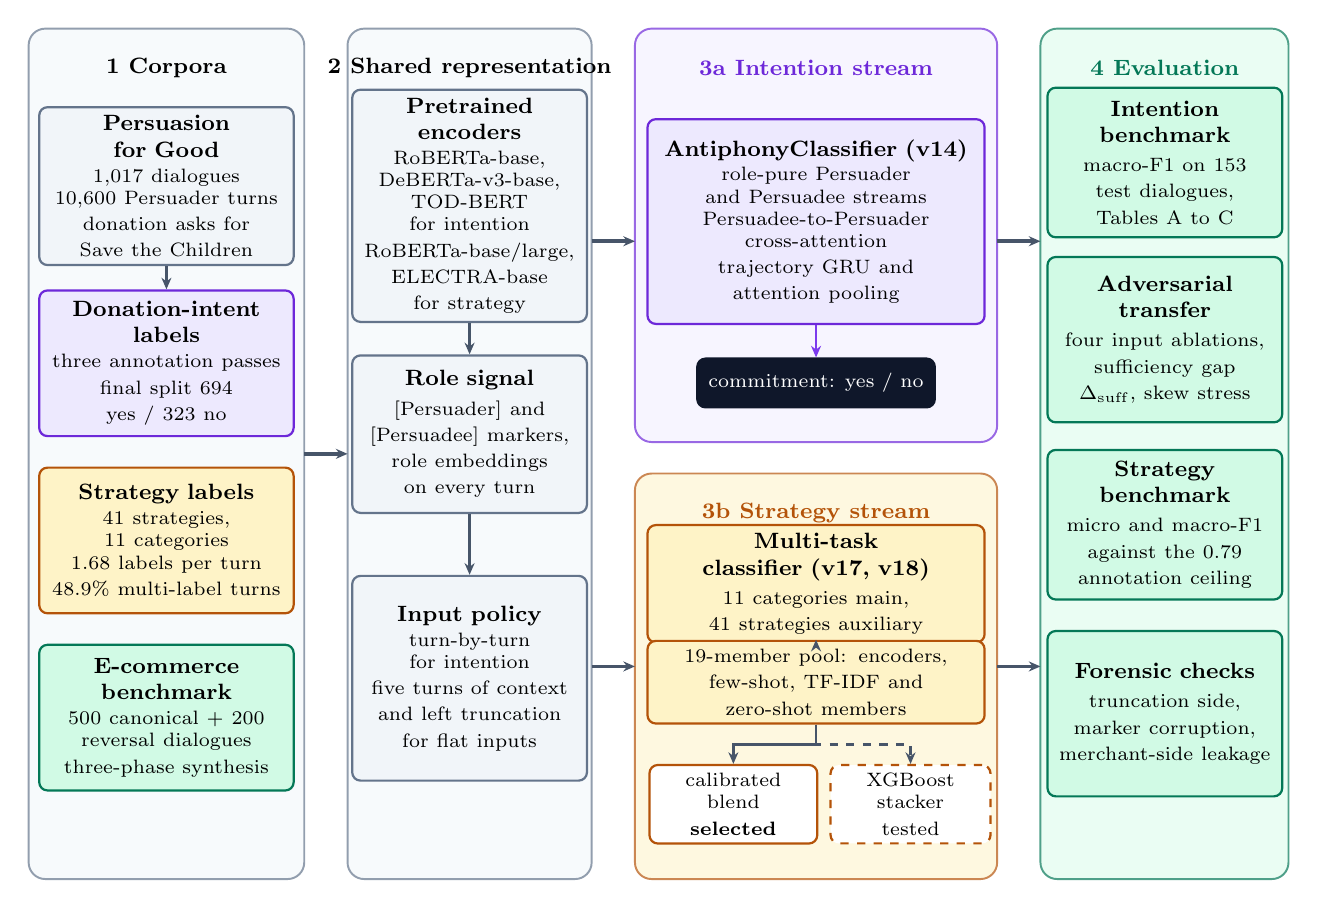
\begin{tikzpicture}[x=1cm,y=1cm]

% ---------------- group backdrops -------------------------------------------------
\draw[rounded corners=6pt, draw=NeuBord!70, fill=NeuFill!55, line width=0.7pt] (0,0.1) rectangle (3.5,-10.7);
\draw[rounded corners=6pt, draw=NeuBord!70, fill=NeuFill!55, line width=0.7pt] (4.05,0.1) rectangle (7.15,-10.7);
\draw[rounded corners=6pt, draw=XatBord!70, fill=XatFill!45, line width=0.7pt] (7.7,0.1) rectangle (12.3,-5.15);
\draw[rounded corners=6pt, draw=AmbBord!70, fill=AmbFill!55, line width=0.7pt] (7.7,-5.55) rectangle (12.3,-10.7);
\draw[rounded corners=6pt, draw=TrjBord!70, fill=TrjFill!45, line width=0.7pt] (12.85,0.1) rectangle (16,-10.7);

\node[ttl] at (1.75,-0.4) {1  Corpora};
\node[ttl] at (5.6,-0.4) {2  Shared representation};
\node[ttl, text=XatBord] at (10.0,-0.4) {3a  Intention stream};
\node[ttl, text=AmbBord] at (10.0,-6.05) {3b  Strategy stream};
\node[ttl, text=TrjBord] at (14.43,-0.4) {4  Evaluation};

% ---------------- 1 corpora -------------------------------------------------------
\node[neu, text width=2.95cm, minimum height=1.85cm] (c1) at (1.75,-1.9)
  {\textbf{Persuasion for Good}\\[1pt]\scriptsize 1{,}017 dialogues\\ 10{,}600 Persuader turns\\ donation asks for Save the Children};
\node[xat, text width=2.95cm, minimum height=1.85cm] (c2) at (1.75,-4.15)
  {\textbf{Donation-intent labels}\\[1pt]\scriptsize three annotation passes\\ final split 694 yes / 323 no};
\node[amb, text width=2.95cm, minimum height=1.85cm] (c3) at (1.75,-6.4)
  {\textbf{Strategy labels}\\[1pt]\scriptsize 41 strategies, 11 categories\\ 1.68 labels per turn\\ 48.9\% multi-label turns};
\node[trj, text width=2.95cm, minimum height=1.85cm] (c4) at (1.75,-8.65)
  {\textbf{E-commerce benchmark}\\[1pt]\scriptsize 500 canonical + 200 reversal dialogues\\ three-phase synthesis};
\draw[flow] (c1) -- (c2);

% ---------------- 2 shared representation ------------------------------------------
\node[neu, text width=2.7cm, minimum height=2.6cm] (r1) at (5.6,-2.15)
  {\textbf{Pretrained encoders}\\[1pt]\scriptsize RoBERTa-base, DeBERTa-v3-base, TOD-BERT for intention\\ RoBERTa-base/large, ELECTRA-base for strategy};
\node[neu, text width=2.7cm, minimum height=2.0cm] (r2) at (5.6,-5.05)
  {\textbf{Role signal}\\[1pt]\scriptsize {[}Persuader{]} and {[}Persuadee{]} markers, role embeddings on every turn};
\node[neu, text width=2.7cm, minimum height=2.6cm] (r3) at (5.6,-8.15)
  {\textbf{Input policy}\\[1pt]\scriptsize turn-by-turn for intention\\ five turns of context and left truncation for flat inputs};
\draw[flow] (r1) -- (r2); \draw[flow] (r2) -- (r3);

% ---------------- 3a intention stream -----------------------------------------------
\node[xat, text width=4.0cm, minimum height=2.6cm] (m1) at (10.0,-2.35)
  {\textbf{AntiphonyClassifier (v14)}\\[1pt]\scriptsize role-pure Persuader and Persuadee streams\\ Persuadee-to-Persuader cross-attention\\ trajectory GRU and attention pooling};
\node[fin, minimum width=2.6cm] (o1) at (10.0,-4.4) {\scriptsize commitment: yes / no};
\draw[flowX] (m1) -- (o1);

% ---------------- 3b strategy stream ------------------------------------------------
\node[amb, text width=4.0cm, minimum height=1.2cm] (s1) at (10.0,-6.95)
  {\textbf{Multi-task classifier (v17, v18)}\\[1pt]\scriptsize 11 categories main, 41 strategies auxiliary};
\node[amb, text width=4.0cm, minimum height=1.0cm] (s2) at (10.0,-8.2)
  {\scriptsize 19-member pool: encoders, few-shot, TF-IDF and zero-shot members};
\node[amb, text width=1.85cm, minimum height=0.95cm, draw=AmbBord, fill=white] (s3a) at (8.95,-9.75)
  {\scriptsize calibrated blend\\ \textbf{selected}};
\node[amb, text width=1.75cm, minimum height=0.95cm, draw=AmbBord, fill=white, dashed] (s3b) at (11.2,-9.75)
  {\scriptsize XGBoost stacker\\ tested};
\draw[flow] (s1) -- (s2);
\draw[flow] (s2.south) -- ++(0,-0.25) -| (s3a.north);
\draw[flow, dashed] (s2.south) -- ++(0,-0.25) -| (s3b.north);

% ---------------- 4 evaluation -----------------------------------------------------
\node[trj, text width=2.7cm, minimum height=1.9cm] (e1) at (14.43,-1.6)
  {\textbf{Intention benchmark}\\[1pt]\scriptsize macro-F1 on 153 test dialogues, Tables A to C};
\node[trj, text width=2.7cm, minimum height=2.1cm] (e2) at (14.43,-3.85)
  {\textbf{Adversarial transfer}\\[1pt]\scriptsize four input ablations, sufficiency gap $\Delta_{\mathrm{suff}}$, skew stress};
\node[trj, text width=2.7cm, minimum height=1.9cm] (e3) at (14.43,-6.2)
  {\textbf{Strategy benchmark}\\[1pt]\scriptsize micro and macro-F1 against the 0.79 annotation ceiling};
\node[trj, text width=2.7cm, minimum height=2.1cm] (e4) at (14.43,-8.6)
  {\textbf{Forensic checks}\\[1pt]\scriptsize truncation side, marker corruption, merchant-side leakage};

% ---------------- inter-group arrows -----------------------------------------------
\draw[flow, line width=1.3pt] (3.5,-5.3) -- (4.05,-5.3);
\draw[flow, line width=1.3pt] (7.15,-2.6) -- (7.7,-2.6);
\draw[flow, line width=1.3pt] (7.15,-8.0) -- (7.7,-8.0);
\draw[flow, line width=1.3pt] (12.3,-2.6) -- (12.85,-2.6);
\draw[flow, line width=1.3pt] (12.3,-8.0) -- (12.85,-8.0);

\end{tikzpicture}
}
  \caption{Overall functional system architecture, illustrating data ingestion across three corpora, shared utterance encoding, the dual-stream Antiphony intention network, the 19-member multi-task strategy classification framework with calibrated decision blending, and the diagnostic ablation evaluation framework.}
  \label{fig:system_architecture}
\end{figure}

\Cref{tab:subsystem-responsibilities} enumerates the functional modules, their inputs, their outputs, and their architectural responsibilities.

\begin{table}[htbp]
  \centering
  \small
  \caption{Modular subsystem decomposition and responsibilities}
  \label{tab:subsystem-responsibilities}
  \begin{tabularx}{\textwidth}{l>{\hsize=0.8\hsize}Y>{\hsize=0.8\hsize}Y>{\hsize=1.4\hsize}Y}
    \toprule
    \textbf{Subsystem} & \textbf{Input} & \textbf{Output} & \textbf{Core Engineering Responsibility} \\
    \midrule
    \textbf{Annotation \& Ground Truth} & Raw text transcripts ($N=1{,}017$, $10{,}600$ turns) & Grounded labels ($y \in \{\text{yes},\text{no}\}$, $\mathbf{y}_t \subseteq \mathcal{S}_{41}$) & Resolves metadata divergence via 3-pass human annotation; enforces 4-tier decision protocol. \\
    \midrule
    \rowcolor{lightbg}
    \textbf{Utterance Encoder} & Batched token IDs $[B \times U, L]$ & Turn matrices $\mathbf{U} \in \mathbb{R}^{B \times U \times d}$ & Executes single batched forward pass; performs masked mean-pooling; enforces memory guards. \\
    \midrule
    \textbf{Strategy Classifier} & Persuader turn $u_t + \mathcal{H}_t$ (5-turn context) & Predicted categories $\hat{\mathbf{c}}_t$ \& strategies $\hat{\mathbf{y}}_t$ & Multi-task learning under Asymmetric Loss; ensembles 19 members via calibrated power-mean blend. \\
    \midrule
    \rowcolor{lightbg}
    \textbf{Antiphony Intention Network} & Full dialogue turn vectors $\mathbf{U}$ & Commitment probability $P(y = \text{yes} \mid \mathcal{D})$ & Role disentanglement ($R=20$); directional cross-attention; trajectory GRU tracking; dual pooling fusion. \\
    \midrule
    \textbf{Diagnostic Ablation Harness} & Full and ablated dialogue streams $\mathbf{H}_M, \mathbf{H}_B$ & Counterfactual ablations (LTR, LTR+M, FHO, PRO), $\Delta_{\text{suff}}$, stress curves & Enforces left-truncation invariant; isolates early merchant accommodation signals; verifies domain-agnostic trajectory necessity. \\
    \bottomrule
  \end{tabularx}
\end{table}

\section{Persuasion Strategy Annotation and Taxonomy}
\label{sec:strategy-annotation}

Modeling the rhetorical tactics that influence conversational outcomes requires an empirically validated, fine-grained taxonomy and a standardized annotation protocol. We establish a multi-label persuasion strategy benchmark encompassing the first $10{,}600$ Persuader turns from $1{,}017$ dialogues in the P4G corpus \cite{wang2019persuasion}.

\subsection{Hierarchical Taxonomy Formulation}
Adapted from social influence theory \cite{cialdini2001influence}, compliance-gaining literature \cite{freedman1966compliance,cialdini1975reciprocal}, and pragmatic dialogue analysis, our taxonomy establishes a two-tier hierarchy: $41$ fine-grained rhetorical strategies nested deterministically under $11$ functional communicative categories (structured in a 4, 4, 4, 4, 3, 4, 4, 3, 3, 4, 4 layout):
\begin{enumerate}[itemsep=2pt,parsep=0pt]
  \item \textbf{Rational Appeal (4 strategies):} \sloppy \texttt{logical\_appeal}, \texttt{evidence\_and\_statistics}, \texttt{cost\_benefit\_framing}, \texttt{feasibility\_and\_ease}.
  \item \textbf{Emotional Appeal (4 strategies):} \sloppy \texttt{emotion\_appeal}, \texttt{guilt\_induction}, \texttt{empathy\_and\_perspective\_taking}, \texttt{hope\_and\_positive\_impact}.
  \item \textbf{Credibility Appeal (4 strategies):} \sloppy \texttt{organizational\_credibility}, \texttt{transparency\_and\_accountability}, \texttt{source\_citation}, \texttt{personal\_credibility}.
  \item \textbf{Social Influence (4 strategies):} \sloppy \texttt{social\_proof}, \texttt{self\_modeling}, \texttt{in\_group\_appeal}, \texttt{authority\_endorsement}.
  \item \textbf{Reciprocity and Exchange (3 strategies):} \sloppy \texttt{reciprocity}, \texttt{donor\_benefit}, \texttt{gratitude\_and\_appreciation}.
  \item \textbf{Commitment and Consistency (4 strategies):} \sloppy \texttt{foot\_in\_the\_door}, \texttt{door\_in\_the\_face}, \texttt{value\_consistency\_appeal}, \texttt{incremental\_ask}.
  \item \textbf{Framing and Presentation (4 strategies):} \sloppy \texttt{anchoring}, \texttt{minimization\_framing}, \texttt{loss\_versus\_gain\_framing}, \texttt{comparison\_framing}.
  \item \textbf{Urgency and Scarcity (3 strategies):} \sloppy \texttt{urgency\_appeal}, \texttt{scarcity\_appeal}, \texttt{deadline\_pressure}.
  \item \textbf{Threat and Pressure (3 strategies):} \sloppy \texttt{negative\_consequence\_warning}, \texttt{persistent\_repetition}, \texttt{obligation\_pressure}.
  \item \textbf{Relational and Interactive (4 strategies):} \sloppy \texttt{rapport\_building}, \texttt{personal\_story}, \texttt{personal\_related\_inquiry}, \texttt{source\_related\_inquiry}.
  \item \textbf{Information Provision (4 strategies):} \sloppy \texttt{organization\_information}, \texttt{donation\_procedure\_information}, \texttt{task\_clarification}, \texttt{impact\_information}.
\end{enumerate}

\subsection{Contextual Annotation Pipeline and Decision Protocol}
Annotating isolated sentences distorts rhetorical meaning; an utterance such as ``Would you be willing to spare 50 cents?'' functions as an \texttt{incremental\_ask} only if preceded by a larger rejected request. Therefore, our pipeline ingests each Persuader utterance within a 5-turn preceding conversational context window ($[u_{t-5}, \dots, u_{t-1}]$) maintaining true speaker alternation.

\begin{figure}[htbp]
  \centering
  \resizebox{\textwidth}{!}{% Multi-label strategy annotation pipeline: 10,600 Persuader turns, 41 strategies, 11 categories.
% Layout: data preparation runs down the left column, then the labelling run flows
% left to right along the bottom row. The supporting groups sit directly above the
% step they act on: decision tests -> prompt, human checkpoints -> labelling and
% validation, merged corpus -> resulting corpus.
% Boxes are stacked with relative positioning and every group backdrop is computed
% with `fit`, so boxes cannot overlap or extend past their group.
% Width is about 16.4 cm; wrap in \resizebox{\textwidth}{!}{...} if the text block is narrower.
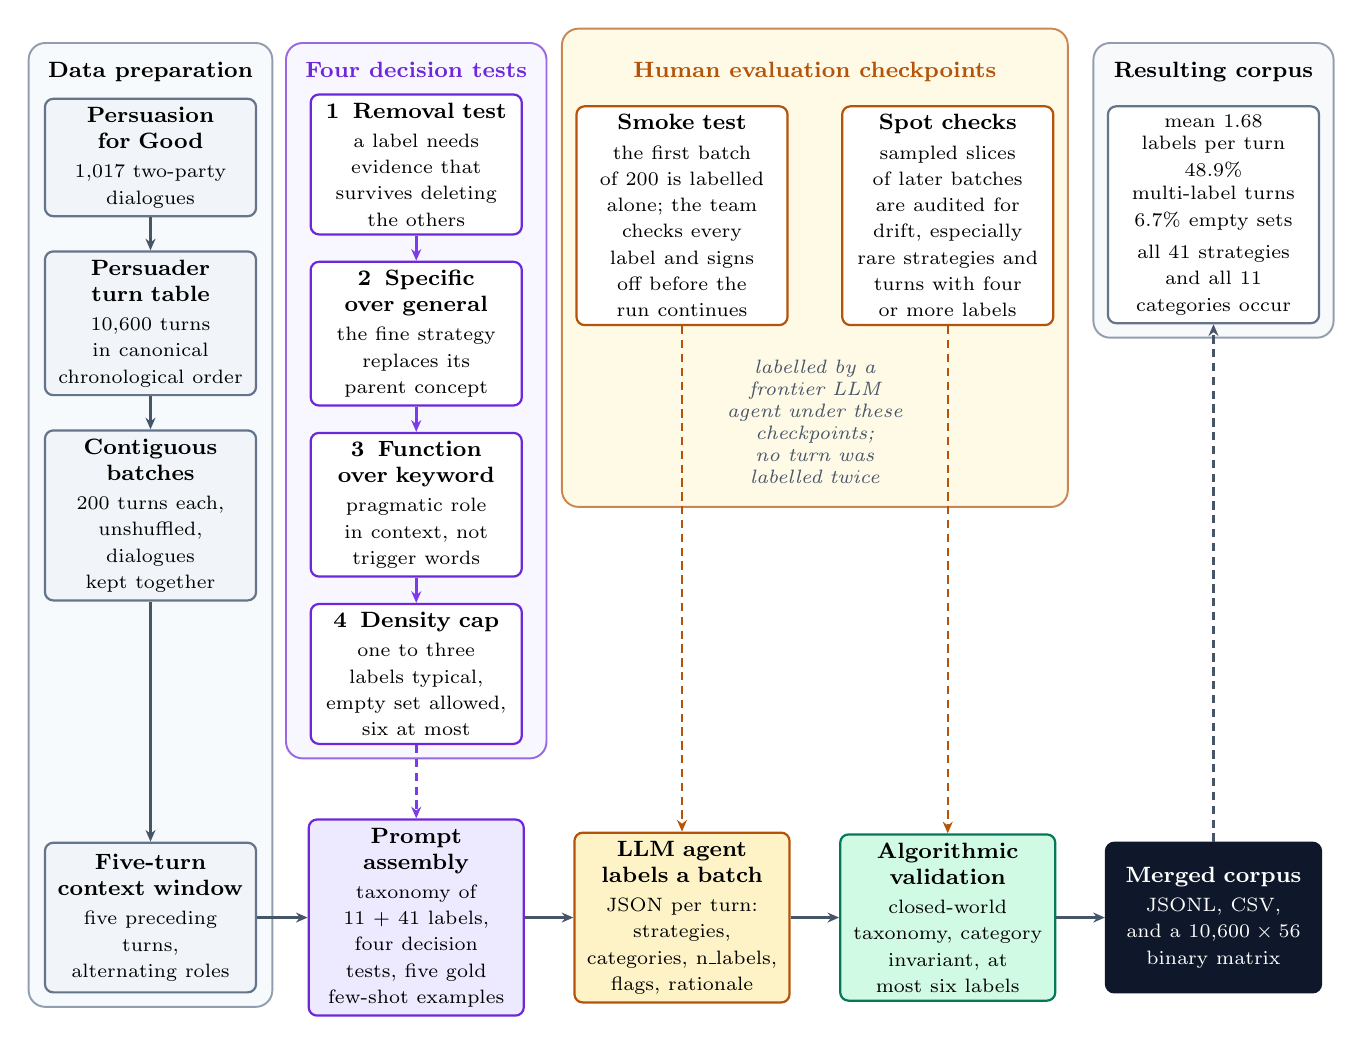
\begin{tikzpicture}[x=1cm,y=1cm, node distance=0.32cm,
  gttl/.style={font=\footnotesize\bfseries, anchor=north, inner sep=2pt},
  band/.style={rounded corners=6pt, line width=0.7pt, inner sep=0.17cm},
  card/.style={blk, fill=white, text width=2.4cm},
  prep/.style={neu, text width=2.4cm},
  stp/.style={text width=2.45cm, minimum height=1.9cm},
  mainflow/.style={flow, line width=1.1pt},
]

% column centres: 5 columns, 2.9 cm wide, 0.475 cm gutters
\def\cA{1.45}\def\cB{4.825}\def\cC{8.2}\def\cD{11.575}\def\cE{14.95}
\coordinate (xA) at (\cA,0); \coordinate (xC) at (\cC,0);
\coordinate (xD) at (\cD,0); \coordinate (xE) at (\cE,0);

% ======================= column 1: data preparation (top to bottom) ================
\node[gttl] (gA) at (\cA,0) {Data preparation};
\node[prep, below=0.12cm of gA] (a1)
  {\textbf{Persuasion for Good}\\[1pt]\scriptsize 1{,}017 two-party dialogues};
\node[prep, below=0.42cm of a1] (a2)
  {\textbf{Persuader turn table}\\[1pt]\scriptsize 10{,}600 turns in canonical chronological order};
\node[prep, below=0.42cm of a2] (a3)
  {\textbf{Contiguous batches}\\[1pt]\scriptsize 200 turns each, unshuffled, dialogues kept together};

% ======================= column 2: four decision tests ==============================
\node[gttl, text=XatBord] (gB) at (\cB,0) {Four decision tests};
\node[xat, card, below=0.12cm of gB] (t1)
  {\textbf{1\enspace Removal test}\\[1pt]\scriptsize a label needs evidence that survives deleting the others};
\node[xat, card, below=of t1] (t2)
  {\textbf{2\enspace Specific over general}\\[1pt]\scriptsize the fine strategy replaces its parent concept};
\node[xat, card, below=of t2] (t3)
  {\textbf{3\enspace Function over keyword}\\[1pt]\scriptsize pragmatic role in context, not trigger words};
\node[xat, card, below=of t3] (t4)
  {\textbf{4\enspace Density cap}\\[1pt]\scriptsize one to three labels typical, empty set allowed, six at most};

% ======================= columns 3-4: human evaluation checkpoints ==================
\coordinate (mCD) at ($(\cC,0)!0.5!(\cD,0)$);
\node[gttl, text=AmbBord] (gC) at (mCD) {Human evaluation checkpoints};
\node[amb, card, anchor=north] (h1) at ($(\cC,0)+(0,-0.62)$)
  {\textbf{Smoke test}\\[1pt]\scriptsize the first batch of 200 is labelled alone; the team checks every label and signs off before the run continues};
\node[amb, card, anchor=north] (h2) at ($(\cD,0)+(0,-0.62)$)
  {\textbf{Spot checks}\\[1pt]\scriptsize sampled slices of later batches are audited for drift, especially rare strategies and turns with four or more labels};
\node[nt, text width=2.55cm, anchor=north] (note) at ($(mCD |- h2.south)+(0,-0.3)$)
  {labelled by a frontier LLM agent under these checkpoints; no turn was labelled twice};

% ======================= column 5: resulting corpus =================================
\node[gttl] (gE) at (\cE,0) {Resulting corpus};
\node[neu, card, anchor=north] (st) at ($(\cE,0)+(0,-0.62)$)
  {\scriptsize mean 1.68 labels per turn\\[2pt] 48.9\% multi-label turns\\[2pt] 6.7\% empty sets\\[2pt] all 41 strategies and all 11 categories occur};

% ======================= top group backdrops (fitted) ===============================
% Groups share a top edge and end at their own natural height.
\begin{scope}[on background layer]
  \node[band, draw=XatBord!70, fill=XatFill!40, fit=(gB)(t1)(t4)] (GB) {};
  \node[band, draw=AmbBord!70, fill=AmbFill!45,
        fit=(gC)(h1)(h2)(note)(GB.north -| h1.west)] (GC) {};
  \node[band, draw=NeuBord!70, fill=NeuFill!60, fit=(gE)(st)] (GE) {};
\end{scope}

% ======================= main row: the labelling run ================================
\node[xat, stp, anchor=north] (b1) at ($(GB.south)+(0,-0.75)$)
  {\textbf{Prompt assembly}\\[1pt]\scriptsize taxonomy of 11 + 41 labels, four decision tests, five gold few-shot examples};
\node[amb, stp] (b2) at (xC |- b1)
  {\textbf{LLM agent labels a batch}\\[1pt]\scriptsize JSON per turn: strategies, categories, n\_labels, flags, rationale};
\node[trj, stp] (b3) at (xD |- b1)
  {\textbf{Algorithmic validation}\\[1pt]\scriptsize closed-world taxonomy, category invariant, at most six labels};
\node[fin, stp] (b4) at (xE |- b1)
  {\textbf{Merged corpus}\\[1pt]\scriptsize JSONL, CSV, and a $10{,}600\times56$ binary matrix};
\node[prep, minimum height=1.9cm] (a4) at (xA |- b1)
  {\textbf{Five-turn context window}\\[1pt]\scriptsize five preceding turns, alternating roles};

\begin{scope}[on background layer]
  \node[band, draw=NeuBord!70, fill=NeuFill!55, fit=(gA)(a1)(a2)(a3)(a4)] (GA) {};
\end{scope}

% ======================= arrows =====================================================
% data preparation, top to bottom
\draw[flow] (a1) -- (a2); \draw[flow] (a2) -- (a3); \draw[flow] (a3) -- (a4);
% main labelling run, left to right
\draw[mainflow] (a4) -- (b1);
\draw[mainflow] (b1) -- (b2);
\draw[mainflow] (b2) -- (b3);
\draw[mainflow] (b3) -- (b4);
% decision tests are written into the prompt
\draw[flowX] (t1) -- (t2); \draw[flowX] (t2) -- (t3); \draw[flowX] (t3) -- (t4);
\draw[flowX, dsh] (t4.south) -- (b1.north);
% human checkpoints act on labelling and validation
\draw[flow, dsh, draw=AmbBord] (h1.south) -- (b2.north);
\draw[flow, dsh, draw=AmbBord] (h2.south) -- (b3.north);
% merged corpus summarised
\draw[flow, dsh] (b4.north) -- (st.south);

\end{tikzpicture}
}
  \caption{Persuasion strategy annotation pipeline, depicting contextual batching (200 turns per batch, 5-turn history), the 4-tier decision protocol, LLM agent annotation under human checkpoints, automated schema validation, and multi-label compilation into \texttt{multilabel\_merged.jsonl}.}
  \label{fig:strategy_annotation_pipeline}
\end{figure}

To eliminate subjective drift and enforce consistency across segments, annotators followed a mandatory \textbf{Four-Tier Decision Protocol} applied in fixed sequential order:
\begin{enumerate}
  \item \textbf{The Removal Test:} A strategy label $\mathbf{s}$ is valid if and only if removing the corresponding clause or rhetorical move noticeably alters the persuasive force or communicative intent of the turn.
  \item \textbf{Specific-over-General Precedence:} If an utterance satisfies both a general category definition (e.g., \texttt{logical\_appeal}) and a highly specific operational tactic (e.g., \texttt{evidence\_and\_statistics} or \texttt{cost\_benefit\_framing}), the specific tactic must be coded, avoiding redundant double-labeling.
  \item \textbf{Pragmatic Function over Keyword Matching:} Labels are assigned based on contextual communicative function rather than literal lexical cues. A rhetorical question (``Don't you want to help a dying child?'') is coded as \texttt{guilt\_induction} and \texttt{emotion\_appeal}, never as an informational inquiry.
  \item \textbf{Realistic Label Density Cap:} While multi-label combinations are expected in complex turns, humans rarely deploy more than three distinct rhetorical tactics simultaneously. The pipeline enforces a typical density of 1 to 3 labels, permits an explicit empty set ($\mathbf{y}_t = \emptyset$) for purely conversational or logistical acknowledgments, and enforces a hard ceiling of $|\mathbf{y}_t| \le 6$.
\end{enumerate}

Annotation was conducted in 200-turn unshuffled batches using an automated frontier LLM agent (Claude 5 Sonnet) driven with few-shot calibration examples, operating under human checkpoints. An automated annotation validation script verified taxonomy compliance, recomputed parent categories from strategies, enforced the label count ceiling, and compiled the verified dataset into \texttt{multilabel\_merged.jsonl} ($10{,}600 \times 56$ wide format with 41 strategy and 11 category flags).

\begin{terminalbox}[Execution Trace: Strategy Annotation Schema Validation]
[+] Ingesting annotated chunks from \texttt{data/raw\_batches/} (10,600 Persuader turns) \\ \relax
[+] Running 4-tier decision constraint harness: \\ \relax
\hspace*{1.5em}- Verifying max strategy density cap: $\max(|\mathbf{y}_t|) \le 6$ \dots\ \textbf{PASS} (mean = 1.68) \\ \relax
\hspace*{1.5em}- Validating deterministic category mapping $\mathcal{M}: \mathcal{S}_{41} \to \mathcal{C}_{11}$ \dots\ \textbf{PASS} (100\% consistent) \\ \relax
\hspace*{1.5em}- Enforcing closed-world vocabulary constraints \dots\ \textbf{PASS} (0 unknown tokens) \\ \relax
\hspace*{1.5em}- Checking speaker alternation invariants \dots\ \textbf{PASS} ($\tau_{\mathcal{P}} = 2t - 1$) \\ \relax
[*] Merging verified batches into \texttt{multilabel\_merged.jsonl} ($10{,}600 \times 56$ matrix) \\ \relax
[+] DATASET AUDIT COMPLETE: 10,600 records serialized, 0 schema violations.
\end{terminalbox}

\subsection{Empirical Corpus Statistics and Rater Effects}
The resulting strategy corpus encompasses $10{,}600$ Persuader turns across $1{,}017$ dialogues (mean $10.42$ Persuader turns per dialogue, range 4 to 15). The dataset exhibits an average of $1.679$ labels per turn ($\text{sd} = 1.061$, median $1.0$). Exactly $707$ turns ($6.7\%$) carry no strategy label (the empty set $\emptyset$), $4{,}707$ turns ($44.4\%$) carry exactly 1 label, and $5{,}182$ turns ($48.9\%$) are multi-label ($\ge 2$ strategies), with 78 turns reaching the maximum cap of 6 labels.

\Cref{tab:category-prevalence} reports the empirical prevalence of all 11 communicative categories, recomputed directly from the data-verified \texttt{multilabel\_merged.jsonl}.

\begin{table}[htbp]
  \centering
  \small
  \caption{Empirical prevalence of communicative categories across 10,600 Persuader turns}
  \label{tab:category-prevalence}
  \begin{tabularx}{\textwidth}{l>{\raggedleft\arraybackslash}X>{\raggedleft\arraybackslash}X}
    \toprule
    \textbf{Communicative Category} & \textbf{Active Turns} & \textbf{Prevalence (\%)} \\
    \midrule
    Relational and Interactive & 4,897 & 46.2\% \\
    \rowcolor{lightbg}
    Information Provision & 3,823 & 36.1\% \\
    Emotional Appeal & 1,645 & 15.5\% \\
    \rowcolor{lightbg}
    Social Influence & 1,263 & 11.9\% \\
    Reciprocity and Exchange & 1,078 & 10.2\% \\
    \rowcolor{lightbg}
    Framing and Presentation & 1,004 & 9.5\% \\
    Credibility Appeal & 896 & 8.5\% \\
    \rowcolor{lightbg}
    Rational Appeal & 751 & 7.1\% \\
    Threat and Pressure & 249 & 2.3\% \\
    \rowcolor{lightbg}
    Commitment and Consistency & 169 & 1.6\% \\
    Urgency and Scarcity & 163 & 1.5\% \\
    \bottomrule
  \end{tabularx}
\end{table}

\textbf{Annotator Granularity Effects:} The corpus was annotated across four distinct operational segments under human checkpoints: Segment 1 (turns 1--2,000; Track A), Segment 2 (turns 2,001--4,000 and 6,001--7,000; Track B), Segment 3 (turns 4,001--6,000; Calibration Track), and Segment 4 (turns 7,001--10,600; Track C). Analysis reveals significant variance in annotation granularity: Track A averaged $2.384$ labels per turn ($9.0\%$ empty sets, $66.8\%$ multi-label), whereas Track C averaged $1.240$ labels per turn ($13.2\%$ empty sets, $30.8\%$ multi-label). This variance represents an operational rater effect in label granularity rather than an intrinsic linguistic shift in the underlying conversations.

\subsection{Derivation of the Cross-Annotator Agreement Ceiling}
Because individual turns were annotated once without global multi-coder duplication, inter-annotator agreement cannot be computed via standard Cohen's kappa. Instead, we derive the empirical performance ceiling from near-duplicate turns across the corpus. On identical or near-identical text pairs (cosine similarity $\ge 0.95$):
\begin{itemize}
  \item When the \textit{same} annotator labels near-identical turns, their self-agreement reaches an F1 of $0.871$.
  \item When \textit{different} annotators label near-identical turns, their cross-agreement drops to an F1 of $0.657$.
\end{itemize}
Because a production model never receives annotator identity at inference time, it must generalize across annotators. Applying consensus prediction formulations under this observed rater noise establishes a practical upper performance ceiling of \textbf{$\approx 0.79$ micro-F1}. All strategy model evaluations must be interpreted relative to this $0.79$ ceiling, where a score of $0.70$ captures nearly $89\%$ of theoretically achievable human consensus.

\section{Conversational Intention Ground Truth Generation}
\label{sec:intention-annotation}

\subsection{The Ground-Truth Divergence Problem}
The original P4G benchmark \cite{wang2019persuasion} recorded numeric donation values reported by Mechanical Turk workers. However, systematic manual auditing revealed severe discrepancies between tabular records and actual conversational text:
\begin{itemize}
  \item In Dialogue \#124, the Persuadee explicitly confirms: `\texttt{We have you down for a \$10 donation. Is that correct?'' / }`Yes that is'', yet the recorded donation amount is \$0.
  \item In Dialogue \#842, the Persuadee states: ``I will absolutely look to donating something later'', while both numeric donation fields show \$0.
\end{itemize}
Training machine learning classifiers on unverified tabular values causes models to learn spurious logging noise rather than genuine conversational commitments.

\begin{figure}[htbp]
  \centering
  \resizebox{\textwidth}{!}{% Three-pass engineering of the donation-intent labels (1,017 dialogues).
% Bar lengths are proportional: 4.6 cm = 1,017 dialogues.
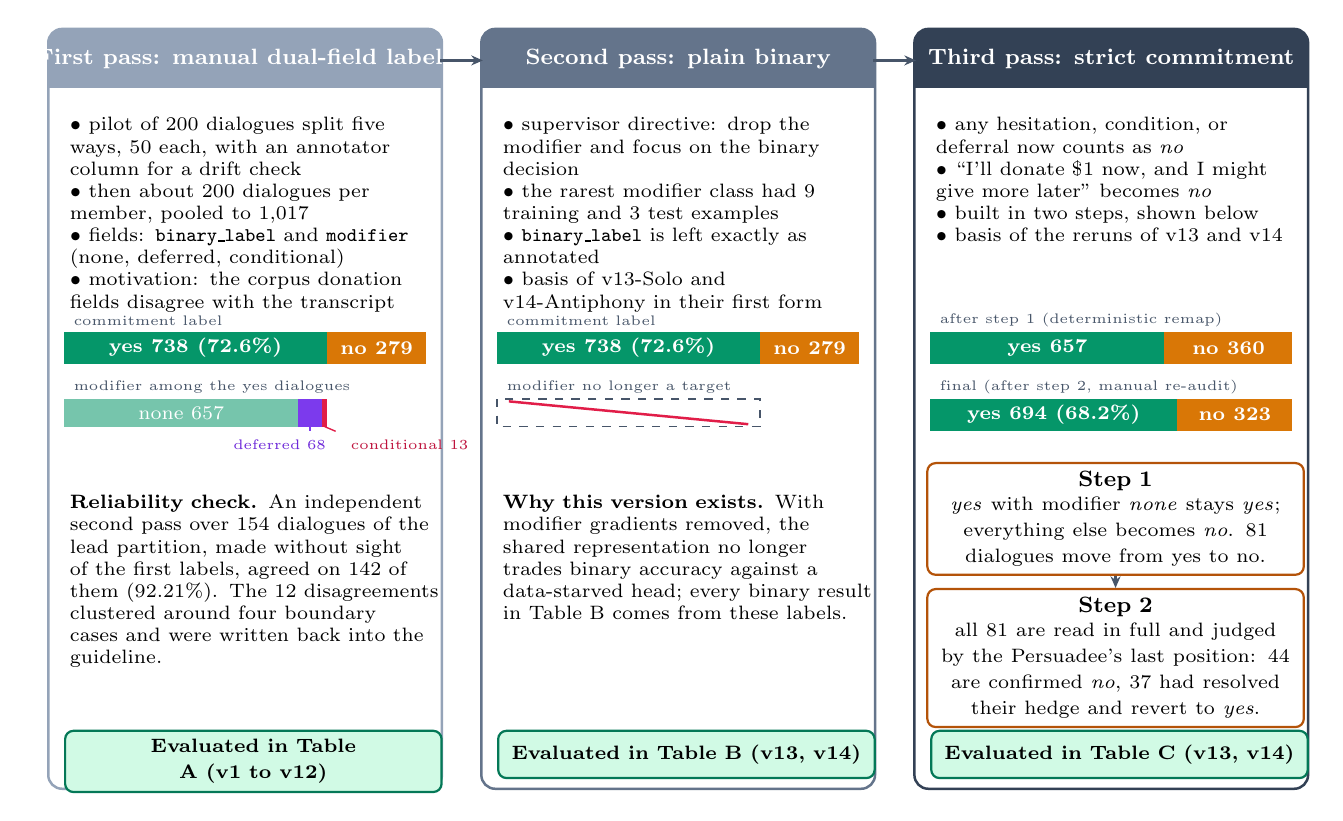
\begin{tikzpicture}[x=1cm,y=1cm]

% ---------------- frames and headers ------------------------------------------------
\foreach \x/\c/\t in {0/94A3B8/{First pass: manual dual-field labels}, 5.5/64748B/{Second pass: plain binary}, 11/334155/{Third pass: strict commitment}}{
  \definecolor{stg}{HTML}{\c}
  \draw[rounded corners=5pt, draw=stg, fill=white, line width=0.9pt] (\x,0.05) rectangle ++(5,-9.65);
  \fill[stg, rounded corners=5pt] (\x,0.05) rectangle ++(5,-0.75);
  \fill[stg] (\x,-0.4) rectangle ++(5,-0.3);
  \node[text=white, font=\footnotesize\bfseries] at (\x+2.5,-0.33) {\t};
}
\foreach \x in {5,10.5}{ \draw[flow, line width=1.3pt] (\x-0.02,-0.35) -- ++(0.54,0); }

% ---------------- body text ---------------------------------------------------------------
\node[anchor=north west, text width=4.7cm, font=\scriptsize, align=left] at (0.15,-0.95)
  {$\bullet$ pilot of 200 dialogues split five ways, 50 each, with an annotator column for a drift check\\
   $\bullet$ then about 200 dialogues per member, pooled to 1{,}017\\
   $\bullet$ fields: \texttt{binary\_label} and \texttt{modifier} (none, deferred, conditional)\\
   $\bullet$ motivation: the corpus donation fields disagree with the transcript};
\node[anchor=north west, text width=4.7cm, font=\scriptsize, align=left] at (5.65,-0.95)
  {$\bullet$ supervisor directive: drop the modifier and focus on the binary decision\\
   $\bullet$ the rarest modifier class had 9 training and 3 test examples\\
   $\bullet$ \texttt{binary\_label} is left exactly as annotated\\
   $\bullet$ basis of v13-Solo and v14-Antiphony in their first form};
\node[anchor=north west, text width=4.7cm, font=\scriptsize, align=left] at (11.15,-0.95)
  {$\bullet$ any hesitation, condition, or deferral now counts as \emph{no}\\
   $\bullet$ ``I'll donate \$1 now, and I might give more later'' becomes \emph{no}\\
   $\bullet$ built in two steps, shown below\\
   $\bullet$ basis of the reruns of v13 and v14};

% ---------------- bars: first pass ------------------------------------------------------------
\begin{scope}[shift={(0.2,0)}]
  \node[font=\tiny, anchor=west, text=SlateSoft] at (0,-3.65) {commitment label};
  \fill[TrjMain] (0,-3.8) rectangle (3.338,-4.2); \fill[AmbMain] (3.338,-3.8) rectangle (4.6,-4.2);
  \node[font=\scriptsize\bfseries, text=white] at (1.67,-4.0) {yes 738 (72.6\%)};
  \node[font=\scriptsize\bfseries, text=white] at (3.97,-4.0) {no 279};
  \node[font=\tiny, anchor=west, text=SlateSoft] at (0,-4.5) {modifier among the yes dialogues};
  \fill[TrjMain!55] (0,-4.65) rectangle (2.972,-5.0);
  \fill[XatMain] (2.972,-4.65) rectangle (3.28,-5.0);
  \fill[PerMain] (3.28,-4.65) rectangle (3.339,-5.0);
  \node[font=\scriptsize, text=white] at (1.49,-4.83) {none 657};
  \node[font=\tiny, anchor=north east, text=XatBord] at (3.45,-5.05) {deferred 68};
  \node[font=\tiny, anchor=north west, text=PerBord] at (3.52,-5.05) {conditional 13};
  \draw[XatMain, line width=0.5pt] (3.126,-5.0) -- (3.126,-5.06); \draw[PerMain, line width=0.5pt] (3.31,-5.0) -- (3.45,-5.06);
\end{scope}

% ---------------- bars: second pass -----------------------------------------------------------
\begin{scope}[shift={(5.7,0)}]
  \node[font=\tiny, anchor=west, text=SlateSoft] at (0,-3.65) {commitment label};
  \fill[TrjMain] (0,-3.8) rectangle (3.338,-4.2); \fill[AmbMain] (3.338,-3.8) rectangle (4.6,-4.2);
  \node[font=\scriptsize\bfseries, text=white] at (1.67,-4.0) {yes 738 (72.6\%)};
  \node[font=\scriptsize\bfseries, text=white] at (3.97,-4.0) {no 279};
  \node[font=\tiny, anchor=west, text=SlateSoft] at (0,-4.5) {modifier no longer a target};
  \draw[SlateSoft, line width=0.6pt, dashed] (0,-4.65) rectangle (3.338,-5.0);
  \draw[PerMain, line width=0.9pt] (0.15,-4.68) -- (3.19,-4.97);
\end{scope}

% ---------------- bars: third pass ------------------------------------------------------------
\begin{scope}[shift={(11.2,0)}]
  \node[font=\tiny, anchor=west, text=SlateSoft] at (0,-3.65) {after step 1 (deterministic remap)};
  \fill[TrjMain] (0,-3.8) rectangle (2.972,-4.2); \fill[AmbMain] (2.972,-3.8) rectangle (4.6,-4.2);
  \node[font=\scriptsize\bfseries, text=white] at (1.49,-4.0) {yes 657};
  \node[font=\scriptsize\bfseries, text=white] at (3.79,-4.0) {no 360};
  \node[font=\tiny, anchor=west, text=SlateSoft] at (0,-4.5) {final (after step 2, manual re-audit)};
  \fill[TrjMain] (0,-4.65) rectangle (3.139,-5.05); \fill[AmbMain] (3.139,-4.65) rectangle (4.6,-5.05);
  \node[font=\scriptsize\bfseries, text=white] at (1.57,-4.85) {yes 694 (68.2\%)};
  \node[font=\scriptsize\bfseries, text=white] at (3.87,-4.85) {no 323};
\end{scope}

% ---------------- third pass, the two steps --------------------------------------------------
\node[amb, fill=white, text width=4.5cm, minimum height=1.25cm, anchor=north west] (s1) at (11.15,-5.45)
  {\textbf{Step 1}\\[-1pt]\scriptsize \emph{yes} with modifier \emph{none} stays \emph{yes}; everything else becomes \emph{no}. 81 dialogues move from yes to no.};
\node[amb, fill=white, text width=4.5cm, minimum height=1.6cm, anchor=north west] (s2) at (11.15,-7.05)
  {\textbf{Step 2}\\[-1pt]\scriptsize all 81 are read in full and judged by the Persuadee's last position: 44 are confirmed \emph{no}, 37 had resolved their hedge and revert to \emph{yes}.};
\draw[flow] (s1.south) -- (s2.north);

% ---------------- what the earlier passes leave open ---------------------------------------
\node[anchor=north west, text width=4.7cm, font=\scriptsize, align=left] at (0.15,-5.75)
  {\textbf{Reliability check.} An independent second pass over 154 dialogues of the lead partition, made without sight of the first labels, agreed on 142 of them (92.21\%). The 12 disagreements clustered around four boundary cases and were written back into the guideline.};
\node[anchor=north west, text width=4.7cm, font=\scriptsize, align=left] at (5.65,-5.75)
  {\textbf{Why this version exists.} With modifier gradients removed, the shared representation no longer trades binary accuracy against a data-starved head; every binary result in Table B comes from these labels.};

% ---------------- where each pass is used -------------------------------------------------------
\foreach \x/\t in {0.2/{Evaluated in Table A (v1 to v12)}, 5.7/{Evaluated in Table B (v13, v14)}, 11.2/{Evaluated in Table C (v13, v14)}}{
  \node[trj, fill=TrjFill, text width=4.5cm, minimum height=0.6cm, anchor=north west] at (\x,-8.85) {\scriptsize\bfseries \t};
}

\end{tikzpicture}
}
  \caption{Three-pass intention annotation lineage, showing the initial 738/279 binary split with modifier, the second pass deprecating the modifier, and the third pass enforcing strict unconditional commitment (694 yes / 323 no via two-step re-checking).}
  \label{fig:intention_annotation_passes}
\end{figure}

\subsection{The Three-Pass Annotation Lineage}
To establish an unassailable ground truth, we executed three successive annotation passes:
\begin{enumerate}
  \item \textbf{First Pass (Dual-Field Manual Annotation):} A pilot of 200 dialogues was split five ways (50 per annotator) with an annotator-tracking column to verify calibration and prevent rater drift. Following calibration, the five team members independently annotated $\approx 200$ dialogues each, reading full transcripts and assigning \texttt{binary\_label} (\texttt{yes}/\texttt{no}) and a \texttt{modifier} (\texttt{none}, \texttt{deferred}, \texttt{conditional}). The pooled 1,017-dialogue distribution yielded: $738$ \texttt{yes} ($72.6\%$) and $279$ \texttt{no} ($27.4\%$). Among affirmative commitments, $657$ were \texttt{none}, $68$ were \texttt{deferred}, and only $13$ were \texttt{conditional} (9 in training, 3 in test).
  \item \textbf{Second Pass (Modifier Deprecation):} Modeling experiments (Chapter 5) proved that the modifier head severely degraded binary performance and suffered from severe data sparsity on the 13-example \texttt{conditional} class. Following a directive from the project supervisor, \SupervisorName, the modifier target was dropped while leaving binary labels unchanged ($738$ \texttt{yes} / $279$ \texttt{no}).
  \item \textbf{Third Pass (Strict Unconditional Commitment):} To create an unambiguous, operationally robust target, the definition of \texttt{yes} was tightened: any hesitation, conditional clause (``if'', ``maybe''), or temporal deferral (``later'') was strictly reclassified as \texttt{no}. This was executed in two steps:
    \begin{itemize}
      \item \textit{Step 1 (Deterministic Remap):} Any dialogue originally marked \texttt{yes} with modifier \texttt{none} remained \texttt{yes}; all dialogues with \texttt{deferred} or \texttt{conditional} modifiers were remapped to \texttt{no}, moving 81 dialogues from \texttt{yes} to \texttt{no} ($657$ \texttt{yes} / $360$ \texttt{no}).
      \item \textit{Step 2 (Terminal Stance Verification):} Because a modifier tag only indicated that a hedge occurred somewhere in the chat, all 81 remapped dialogues were manually re-read in full to evaluate their final state. If an early hesitation was cleanly resolved into an unconditional affirmative by the end, it was reverted to \texttt{yes}. Exactly 44 dialogues were confirmed as \texttt{no}, and 37 were reverted to \texttt{yes}.
    \end{itemize}
    The finalized third-pass ground truth contains exactly \textbf{694 \texttt{yes} ($68.2\%$) / 323 \texttt{no} ($31.8\%$)}.
\end{enumerate}

\subsection{Inter-Annotator Agreement and Boundary Cases}
An independent second-pass annotation over 154 dialogues established an inter-annotator agreement rate of \textbf{$92.21\%$} (142 of 154 identical assignments). Qualitative review of the 12 boundary disagreements revealed four recurring linguistic phenomena: (i) ambiguous temporal deferrals (``I'll donate through their website tonight''), (ii) polite deflection masquerading as consent (``Sure, that sounds like a great cause''), (iii) conditional matches (``I'll give \$1 if you give \$1''), and (iv) unconfirmed donation queries. Adjudicating these boundary cases under the strict third-pass standard eliminated residual ambiguity.

\section{Synthetic E-Commerce Negotiation Benchmark}
\label{sec:synthetic-benchmark}

\subsection{Motivation and Privacy Bottlenecks}
Evaluating cross-domain generalization from charitable persuasion to commercial negotiation is obstructed by data access barriers: private customer-merchant chat logs on platforms like WhatsApp or Facebook Messenger are legally protected under privacy statutes and commercially sensitive. To enable rigorous, leak-free evaluation, we designed a three-phase synthetic benchmark generation pipeline producing 700 fully audited negotiation dialogues.

\begin{figure}[htbp]
  \centering
  \resizebox{\textwidth}{!}{% Three-phase synthetic e-commerce negotiation benchmark: synthesis, humanisation, audit.
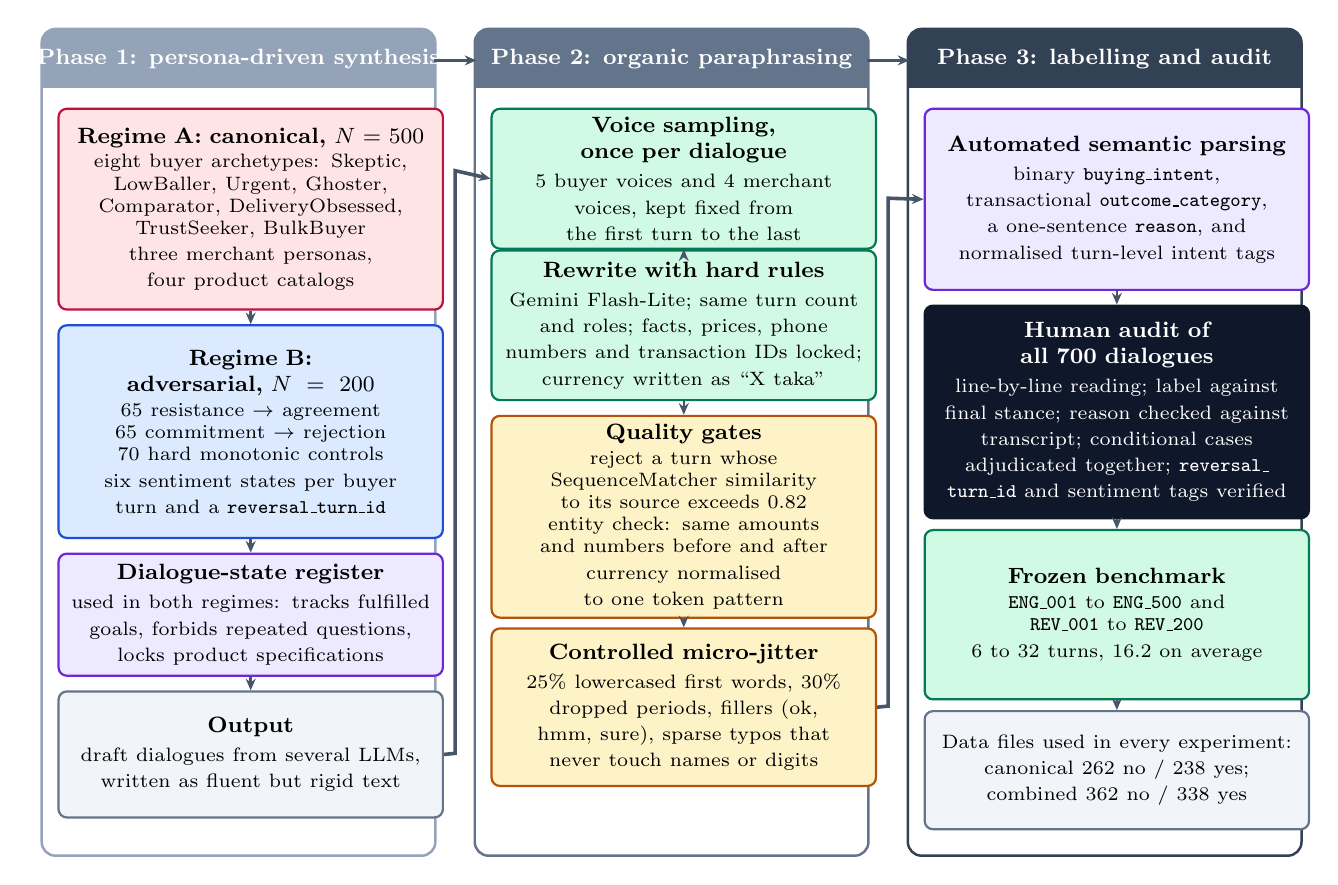
\begin{tikzpicture}[x=1cm,y=1cm]

% ---------------- phase frames ---------------------------------------------------------------
\foreach \x/\c/\t in {0/94A3B8/{Phase 1: persona-driven synthesis}, 5.5/64748B/{Phase 2: organic paraphrasing}, 11/334155/{Phase 3: labelling and audit}}{
  \definecolor{stg}{HTML}{\c}
  \draw[rounded corners=5pt, draw=stg, fill=white, line width=0.9pt] (\x,0.05) rectangle ++(5,-10.5);
  \fill[stg, rounded corners=5pt] (\x,0.05) rectangle ++(5,-0.75);
  \fill[stg] (\x,-0.4) rectangle ++(5,-0.3);
  \node[text=white, font=\footnotesize\bfseries] at (\x+2.5,-0.33) {\t};
}
\foreach \x in {5,10.5}{ \draw[flow, line width=1.3pt] (\x-0.02,-0.35) -- ++(0.54,0); }

% =============== phase 1 ==========================================================================
\node[per, text width=4.6cm, minimum height=2.55cm, anchor=north west] (r1) at (0.2,-0.95)
  {\textbf{Regime A: canonical, $N=500$}\\[1pt]\scriptsize eight buyer archetypes: Skeptic, LowBaller, Urgent, Ghoster, Comparator, DeliveryObsessed, TrustSeeker, BulkBuyer\\ three merchant personas, four product catalogs};
\node[dec, text width=4.6cm, minimum height=2.7cm, anchor=north west] (r2) at (0.2,-3.7)
  {\textbf{Regime B: adversarial, $N=200$}\\[1pt]\scriptsize 65 resistance $\to$ agreement\\ 65 commitment $\to$ rejection\\ 70 hard monotonic controls\\ six sentiment states per buyer turn and a \texttt{reversal\_turn\_id}};
\node[xat, text width=4.6cm, minimum height=1.55cm, anchor=north west] (r3) at (0.2,-6.6)
  {\textbf{Dialogue-state register}\\[1pt]\scriptsize used in both regimes: tracks fulfilled goals, forbids repeated questions, locks product specifications};
\node[neu, text width=4.6cm, minimum height=1.6cm, anchor=north west] (r4) at (0.2,-8.35)
  {\textbf{Output}\\[1pt]\scriptsize draft dialogues from several LLMs, written as fluent but rigid text};
\draw[flow] (r1.south) -- (r2.north);
\draw[flow] (r2.south) -- (r3.north);
\draw[flow] (r3.south) -- (r4.north);

% =============== phase 2 ==========================================================================
\node[trj, text width=4.6cm, minimum height=1.6cm, anchor=north west] (p1) at (5.7,-0.95)
  {\textbf{Voice sampling, once per dialogue}\\[1pt]\scriptsize 5 buyer voices and 4 merchant voices, kept fixed from the first turn to the last};
\node[trj, text width=4.6cm, minimum height=1.9cm, anchor=north west] (p2) at (5.7,-2.75)
  {\textbf{Rewrite with hard rules}\\[1pt]\scriptsize Gemini Flash-Lite; same turn count and roles; facts, prices, phone numbers and transaction IDs locked; currency written as ``X taka''};
\node[amb, text width=4.6cm, minimum height=2.5cm, anchor=north west] (p3) at (5.7,-4.85)
  {\textbf{Quality gates}\\[1pt]\scriptsize reject a turn whose SequenceMatcher similarity to its source exceeds 0.82\\ entity check: same amounts and numbers before and after\\ currency normalised to one token pattern};
\node[amb, text width=4.6cm, minimum height=2.0cm, anchor=north west] (p4) at (5.7,-7.55)
  {\textbf{Controlled micro-jitter}\\[1pt]\scriptsize 25\% lowercased first words, 30\% dropped periods, fillers (ok, hmm, sure), sparse typos that never touch names or digits};
\draw[flow] (p1) -- (p2); \draw[flow] (p2) -- (p3); \draw[flow] (p3) -- (p4);

% =============== phase 3 ==========================================================================
\node[xat, text width=4.6cm, minimum height=2.3cm, anchor=north west] (l1) at (11.2,-0.95)
  {\textbf{Automated semantic parsing}\\[1pt]\scriptsize binary \texttt{buying\_intent}, transactional \texttt{outcome\_category}, a one-sentence \texttt{reason}, and normalised turn-level intent tags};
\node[fin, text width=4.6cm, minimum height=2.7cm, anchor=north west] (l2) at (11.2,-3.45)
  {\textbf{Human audit of all 700 dialogues}\\[1pt]\scriptsize line-by-line reading; label against final stance; reason checked against transcript; conditional cases adjudicated together; \texttt{reversal\_turn\_id} and sentiment tags verified};
\node[trj, text width=4.6cm, minimum height=2.15cm, anchor=north west] (l3) at (11.2,-6.3)
  {\textbf{Frozen benchmark}\\[1pt]\scriptsize \texttt{ENG\_001} to \texttt{ENG\_500} and \texttt{REV\_001} to \texttt{REV\_200}\\ 6 to 32 turns, 16.2 on average};
\draw[flow] (l1) -- (l2); \draw[flow] (l2) -- (l3);
\node[neu, text width=4.6cm, minimum height=1.5cm, anchor=north west] (l4) at (11.2,-8.6)
  {\scriptsize Data files used in every experiment: canonical 262 no / 238 yes; combined 362 no / 338 yes};
\draw[flow, dashed] (l3.south) -- (l4.north);

% ---------------- long connectors -------------------------------------------------------------------
\draw[flow, line width=1.3pt] (r4.east) -- (5.25,-9.15) -- (5.25,-1.75) -- (p1.west);
\draw[flow, line width=1.3pt] (p4.east) -- (10.75,-8.55) -- (10.75,-2.1) -- (l1.west);

\end{tikzpicture}
}
  \caption{Three-phase synthetic negotiation benchmark generation pipeline, comprising persona-conditioned LLM drafting ($N=500$ canonical, $N=200$ adversarial reversals), organic paraphrasing with linguistic jitter, and multi-tier semantic audit.}
  \label{fig:datagen_pipeline}
\end{figure}

\subsection{The Three-Phase Generation Framework}
\begin{enumerate}
  \item \textbf{Phase 1: Persona-Conditioned Prompt-Driven Synthesis:} Dialogues are generated under two distinct regimes across multiple LLM backbones (including Qwen-2.5):
    \begin{itemize}
      \item \textit{Regime A (Canonical Stream, $N=500$):} Models standard consumer transactions across eight behavioral buyer archetypes (The Skeptic, The LowBaller, The Urgent Buyer, The Ghoster, The Comparator, The DeliveryObsessed, The TrustSeeker, The BulkBuyer), three professional merchant personas (courteous page admin, small shopkeeper, formal retail representative), and four consumer product categories (electronics/phones, traditional apparel, home appliances, organic specialty goods). A Dialogue State Tracking (DST) register prevents repetitive loops.
      \item \textit{Regime B (Adversarial Reversal Stream, $N=200$):} Generates non-monotonic trajectory shifts: 65 positive reversals (\texttt{resistance\_to\_agreement}, where deep skepticism resolves after a verified warranty), 65 negative reversals (\texttt{commit\_to\_rejection}, where early commitment collapses over delivery fees), and 70 hard monotonic controls designed with identical lengths and friction to prevent models from learning length-based shortcuts.
    \end{itemize}
  \item \textbf{Phase 2: Organic Paraphrasing and Humanization:} To strip away synthetic LLM phrasing and replicate mobile messaging dynamics, drafts pass through an organic paraphrasing engine powered by the Gemini API (\texttt{gemini-3.5-flash-lite}). The engine injects controlled linguistic jitter: 25\% lowercased sentence openers, 30\% dropped terminal periods, natural fillers (``hmm'', ``well'', ``ok''), local pricing terms (``X taka''), and sparse typos that strictly protect product names and digits. A strict similarity gate rejects any rewritten turn with a SequenceMatcher ratio $>0.82$ against the source draft.
  \item \textbf{Phase 3: Semantic Labeling and 100\% Team Audit:} An automated pass assigns \texttt{buying\_intent}, multi-class \texttt{outcome\_category}, and textual justifications. The entire research team then conducted an exhaustive 100\% manual audit of all 700 dialogues, verifying stance consistency, correcting subtle hallucinations, and confirming reversal turn IDs ($\tau_{\text{rev}}$).
\end{enumerate}

\subsection{Frozen Benchmark Dataset Counts}
While early design prompts envisioned a 250/250 canonical split across six outcome classes, the finalized, frozen datasets utilized in all experimental runs contain verified counts across four primary outcome categories:
\begin{itemize}
  \item \textbf{Canonical Benchmark ($N=500$):} $262$ \texttt{no} ($52.4\%$) / $238$ \texttt{yes} ($47.6\%$). Outcomes: \texttt{PURCHASE\_COMMITTED} 238, \texttt{DEFERRED\_CONSIDERATION} 139, \texttt{INQUIRY\_DROPOUT} 112, \texttt{EXPLICIT\_REJECTION} 11. Mean turns: $15.9$ (range 6 to 32).
  \item \textbf{Adversarial Reversals ($N=200$):} Exactly $100$ \texttt{no} / $100$ \texttt{yes}. Mean turns: $17.1$ (range 8 to 30).
  \item \textbf{Combined Augmented Benchmark ($N=700$):} $362$ \texttt{no} ($51.7\%$) / $338$ \texttt{yes} ($48.3\%$). Outcomes: \texttt{PURCHASE\_COMMITTED} 338, \texttt{DEFERRED\_CONSIDERATION} 157, \texttt{INQUIRY\_DROPOUT} 125, \texttt{EXPLICIT\_REJECTION} 80. Mean turns: $16.2$ (range 6 to 32).
\end{itemize}

\subsection{Generic Architecture Diagnostic and Ablation Harness}
\label{sec:diagnostic-ablation-harness}

To determine whether the architectural mechanisms in Antiphony (speaker disentanglement, directional cross-attention, and trajectory tracking) reflect genuine domain-agnostic inductive biases for asymmetric multi-turn dialogue rather than overfitting to donation persuasion, we engineered a dedicated generic architecture diagnostic and ablation harness.

\subsubsection{Counterfactual Input-Ablation Operators}
In conversational benchmarks, conversational outcomes can easily become overdetermined: explicit affirmations or closing logistical exchanges allow flat sequence classifiers to infer intent from isolated surface tokens, bypassing dialogue history. To systematically pinpoint the causal source of predictive representations, the harness formalizes four distinct counterfactual input-ablation operators:
\begin{enumerate}
  \item \textbf{Last-Turn-Removed ($\text{Ablation}_{\text{LTR}}$):} Excises the final decider turn:
    \begin{equation}
      \mathcal{D}_{\text{LTR}} = \mathcal{D} \setminus \{u_{\text{final}}\}
    \end{equation}
    This evaluates whether preceding conversational momentum enables outcome inference without an explicit closing declaration.
  \item \textbf{Last-Turn and Merchant Courtesy Removed ($\text{Ablation}_{\text{LTR+M}}$):} In commercial transactions, merchants routinely emit closing courtesy affirmations (payment receipts, shipping notices) immediately following agreement. This operator excises both the terminal buyer turn and any trailing merchant courtesy turns:
    \begin{equation}
      \mathcal{D}_{\text{LTR+M}} = \mathcal{D} \setminus \{u \in \mathcal{D} \mid \text{index}(u) \ge \text{index}(u_{\text{final}})\}
    \end{equation}
    thereby completely severing closing bidirectional lexical leakage.
  \item \textbf{First-Half-Only ($\text{Ablation}_{\text{FHO}}$):} Dialogues are restricted strictly to the first $50\%$ of turns ($u_1, \dots, u_{\lfloor K/2 \rfloor}$), detecting early predictive bias and verifying that synthetic personas do not leak the outcome in the initial exchanges.
  \item \textbf{Pre-Reversal-Only ($\text{Ablation}_{\text{PRO}}$):} Applied to adversarial reversal dialogues exhibiting an annotated stance-shift at turn $\tau_{\text{rev}}$, this operator excises all content from the shift onward:
    \begin{equation}
      \mathcal{D}_{\text{PRO}} = [u_1, \dots, u_{\tau_{\text{rev}} - 1}]
    \end{equation}
    testing whether models commit prematurely to initial buyer resistance or correctly exploit merchant accommodation signals.
\end{enumerate}

\subsubsection{Tokenizer Truncation Directionality Invariant}
During the engineering of the ablation harness, a critical diagnostic defect was exposed: standard transformer tokenization libraries apply right-truncation by default (\texttt{truncation\_side='right'}, capped at 512 tokens). In lengthy multi-turn commercial chats ($30.4\%$ of dialogues in the benchmark exceeded 512 tokens), right-truncation silently discards the terminal tail of the conversation. When applying $\text{Ablation}_{\text{LTR}}$, right-truncated tokenizers mistakenly pruned the proximal turns preceding the excised turn, generating an artificial $+0.1600$ necessity collapse (Macro-F1 plunging to $0.8133$).

The diagnostic harness enforces a strict \textbf{left-truncation invariant} (\texttt{truncation\_side='left'}):
\begin{equation}
  \text{Tokens}(\mathcal{D}) = [t_{\max(1, N_{\text{tokens}} - L_{\max} + 1)}, \dots, t_{N_{\text{tokens}}}]
\end{equation}
which discards only early introductory pleasantries while strictly preserving the vital decision-boundary turns. Enforcing this invariant recovered baseline performance to $0.9331$, establishing that the true necessity gap on canonical dialogues is modest ($+0.0402$).

\subsubsection{Parametric Skew-Stress Formulation}
To evaluate operational resilience against severe real-world class imbalance without retraining the shared encoder, the harness implements a parametric class-pruning generator. Given a balanced training distribution ($47.7\%$ affirmative, $n=350$), affirmative dialogues are subsampled according to target ratio $\alpha \in [0.10, 0.50]$:
\begin{equation}
  n_{\text{pos}} = \left\lfloor \frac{\alpha}{1 - \alpha} \cdot n_{\text{neg}} \right\rfloor
\end{equation}
depressing the affirmative training ratio down to $9.85\%$ ($n=203$). This profiles how gracefully directional cross-attention and recurrent trajectory tracking maintain calibration compared to flat sequence models under operational distribution collapse.

\section{Strategy and Category Modeling Architecture}
\label{sec:strategy-modeling}

Predicting multi-label rhetorical strategies across an extreme long tail requires a multi-task formulation supported by an ensemble of diverse base learners and a calibrated decision layer.

\begin{figure}[htbp]
  \centering
  \resizebox{\textwidth}{!}{% Strategy / category classifier (v18): how the 19-member pool is built and decided.
% Three stacked bands, read top to bottom:
%   1. one ensemble member: the transformer recipe (runs 7 times)
%   2. the pool of 19 members, grouped by how each is built
%   3. the decision layer that turns 19 probabilities into a label set
% Uses the shared palette and styles from tikzstyles.tex (amber = strategy stream,
% green = few-shot companions, neutral = classical / zero-shot, slate = outputs).
% Width is about 16.4 cm; needs amssymb for \mathbb.
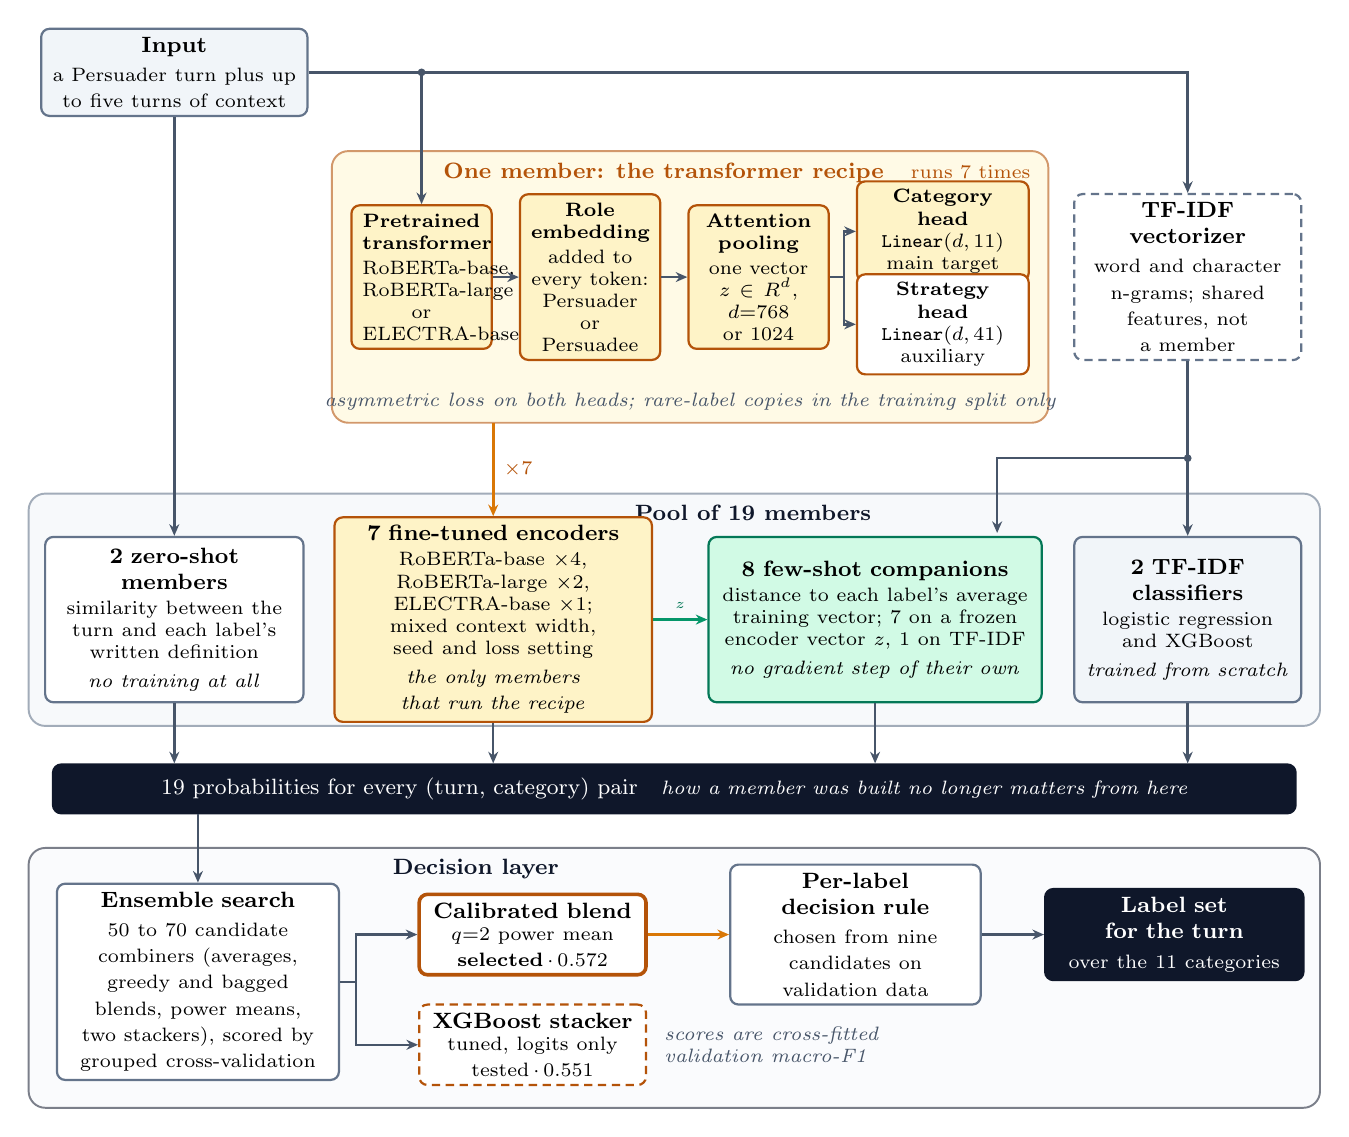
\begin{tikzpicture}[x=1cm,y=1cm,
  band/.style={rounded corners=6pt, line width=0.7pt},
  btitle/.style={font=\footnotesize\bfseries, inner sep=2pt},
  sub/.style={font=\scriptsize},
  rstep/.style={amb, text width=1.5cm, minimum height=1.55cm, font=\scriptsize},
  member/.style={minimum height=2.1cm},
  bigflow/.style={flow, line width=1.1pt},
]

% ======================= band backdrops =============================================
\draw[band, draw=AmbBord!60, fill=AmbFill!45] (3.85,-1.0) rectangle (12.95,-4.45);
\draw[band, draw=NeuBord!60, fill=NeuFill!60] (0,-5.35) rectangle (16.4,-8.3);
\draw[band, draw=Slate!55, fill=NeuFill!35] (0,-9.85) rectangle (16.4,-13.15);

\node[btitle, text=AmbBord, anchor=north east] at (12.8,-1.08)
  {One member: the transformer recipe\quad{\normalfont\scriptsize runs 7 times}};
\node[btitle, text=Slate, anchor=north] at (9.2,-5.42) {Pool of 19 members};
\node[btitle, text=Slate, anchor=north west] at (4.55,-9.92) {Decision layer};

% ======================= input ======================================================
\node[neu, text width=3.1cm] (in) at (1.85,0)
  {\textbf{Input}\\[1pt]\scriptsize a Persuader turn plus up to five turns of context};

% ======================= band 1: transformer recipe =================================
\node[rstep] (t1) at (4.99,-2.6)
  {\textbf{Pretrained transformer}\\[1pt] RoBERTa-base, RoBERTa-large or ELECTRA-base};
\node[rstep] (t2) at (7.13,-2.6)
  {\textbf{Role embedding}\\[1pt] added to every token: Persuader or Persuadee};
\node[rstep] (t3) at (9.27,-2.6)
  {\textbf{Attention pooling}\\[1pt] one vector $z\in\mathbb{R}^d$, $d{=}768$ or $1024$};
\node[amb, text width=1.9cm, font=\scriptsize] (hc) at (11.61,-2.02)
  {\textbf{Category head}\\ \mbox{\texttt{Linear}($d$,\,11)}\\ main target};
\node[amb, fill=white, text width=1.9cm, font=\scriptsize] (hs) at (11.61,-3.2)
  {\textbf{Strategy head}\\ \mbox{\texttt{Linear}($d$,\,41)}\\ auxiliary};
\draw[flow] (t1) -- (t2);
\draw[flow] (t2) -- (t3);
\draw[flow] (t3.east) -- ++(0.18,0) |- (hc.west);
\draw[flow] (t3.east) -- ++(0.18,0) |- (hs.west);
\node[nt, anchor=south] at (8.4,-4.42)
  {asymmetric loss on both heads; rare-label copies in the training split only};

% ======================= TF-IDF vectorizer (shared features, not a member) ==========
\node[neu, fill=white, dsh, text width=2.6cm] (vec) at (14.72,-2.6)
  {\textbf{TF-IDF vectorizer}\\[1pt]\scriptsize word and character n-grams; shared features, not a member};

% ======================= band 2: the 19 members =====================================
\node[neu, fill=white, member, text width=3.0cm] (zs) at (1.85,-6.95)
  {\textbf{2 zero-shot members}\\[1pt]\scriptsize similarity between the turn and each label's written definition\\[1pt]\textit{no training at all}};
\node[amb, member, text width=3.75cm] (enc) at (5.9,-6.95)
  {\textbf{7 fine-tuned encoders}\\[1pt]\scriptsize RoBERTa-base $\times4$, RoBERTa-large $\times2$, ELECTRA-base $\times1$; mixed context width, seed and loss setting\\[1pt]\textit{the only members that run the recipe}};
\node[trj, member, text width=3.95cm] (fs) at (10.75,-6.95)
  {\textbf{8 few-shot companions}\\[1pt]\scriptsize distance to each label's average training vector; 7 on a frozen encoder vector $z$, 1 on TF-IDF\\[1pt]\textit{no gradient step of their own}};
\node[neu, member, text width=2.6cm] (tc) at (14.72,-6.95)
  {\textbf{2 TF-IDF classifiers}\\[1pt]\scriptsize logistic regression and XGBoost\\[1pt]\textit{trained from scratch}};

% ======================= band 3: decision layer =====================================
\node[fin, text width=15.5cm] (probs) at (8.2,-9.1)
  {19 probabilities for every (turn, category) pair\quad{\scriptsize\itshape how a member was built no longer matters from here}};

\node[neu, fill=white, text width=3.3cm, minimum height=2.3cm] (ens) at (2.15,-11.55)
  {\textbf{Ensemble search}\\[1pt]\scriptsize 50 to 70 candidate combiners (averages, greedy and bagged blends, power means, two stackers), scored by grouped cross-validation};
\node[amb, fill=white, line width=1.3pt, text width=2.6cm] (bl) at (6.4,-10.95)
  {\textbf{Calibrated blend}\\\scriptsize $q{=}2$ power mean\\ \textbf{selected}\,$\cdot$\,0.572};
\node[amb, fill=white, dsh, text width=2.6cm] (xg) at (6.4,-12.35)
  {\textbf{XGBoost stacker}\\\scriptsize tuned, logits only\\ tested\,$\cdot$\,0.551};
\node[neu, fill=white, text width=2.9cm] (rule) at (10.5,-10.95)
  {\textbf{Per-label decision rule}\\[1pt]\scriptsize chosen from nine candidates on validation data};
\node[fin, text width=3.0cm] (out) at (14.55,-10.95)
  {\textbf{Label set for the turn}\\[1pt]\scriptsize over the 11 categories};
\node[nt, anchor=west, align=left] at (7.95,-12.35) {scores are cross-fitted\\validation macro-F1};

% ======================= arrows =====================================================
% input feeds the recipe, the TF-IDF vectorizer and the zero-shot members
\draw[flow] (in.east) -- (14.72,0) -- (vec.north);
\draw[flow] (4.99,0) -- (t1.north);
\fill[SlateSoft] (4.99,0) circle (1.4pt);
\draw[flow] (in.south) -- (zs.north);

% recipe -> the 7 encoders
\draw[bigflow, draw=AmbMain] (5.9,-4.45) -- node[right, font=\scriptsize\bfseries, text=AmbBord]{$\times 7$} (enc.north);

% TF-IDF vectorizer -> TF-IDF classifiers and the 8th few-shot companion
\draw[flow] (vec.south) -- (tc.north);
\draw[flow] (14.72,-4.9) -- (12.3,-4.9) -- (12.3,-5.85);
\fill[SlateSoft] (14.72,-4.9) circle (1.4pt);

% encoders -> few-shot companions (frozen vector z)
\draw[flowT] (enc.east) -- node[above, font=\tiny, text=TrjBord]{$z$} (fs.west);

% every member group -> the 19 probabilities
\foreach \m in {zs,enc,fs,tc}{ \draw[flow] (\m.south) -- (\m.south |- probs.north); }

% decision layer
\draw[flow] (probs.south -| ens.north) -- (ens.north);
\draw[flow] (ens.east) -- ++(0.2,0) |- (bl.west);
\draw[flow] (ens.east) -- ++(0.2,0) |- (xg.west);
\draw[bigflow, draw=AmbMain] (bl) -- (rule);
\draw[bigflow] (rule) -- (out);

\end{tikzpicture}
}
  \caption{Strategy and category classification framework, illustrating the 19-member model pool, multi-task representation heads, and decision layer search comparing calibrated power-mean blending (selected, val macro-F1 0.5716) against XGBoost stacking (tested, val macro-F1 0.5508).}
  \label{fig:strategy_model}
\end{figure}

\subsection{Multi-Task Category-First Formulation}
Because the 41 strategies include classes with as few as 2 examples (\texttt{door\_in\_the\_face}), models trained solely on 41 fine strategies achieve poor macro-F1 ($0.368$). We pivot the primary modeling target to the 11 communicative categories, where every category has over 100 real instances. We formulate a multi-task network where the 11 categories act as the primary objective ($\mathcal{L}_{\text{cat}}$) and the 41 strategies act as an auxiliary regularizer ($\mathcal{L}_{\text{strat}}$):
\begin{equation}
  \mathcal{L}_{\text{total}} = \mathcal{L}_{\text{cat}} + \lambda_{\text{aux}} \mathcal{L}_{\text{strat}}
\end{equation}
with $\lambda_{\text{aux}} \in [0.1, 0.3]$. Both heads are optimized using Asymmetric Loss (ASL) \cite{benbaruch2021asymmetric}:
\begin{equation}
  \mathcal{L}_{\text{ASL}} = -\sum_{c=1}^{C} \left[ y_c (1 - p_c)^{\gamma_+} \log(p_c) + (1 - y_c) (p_{m,c})^{\gamma_-} \log(1 - p_{m,c}) \right]
\end{equation}
where $p_{m,c} = \max(p_c - m, 0)$ incorporates hard probability margin shifting ($m=0.05$) and asymmetric focusing ($\gamma_+ = 0, \gamma_- = 4$) to discard easy negative gradients.

\subsection{The 19-Member Heterogeneous Model Pool}
To maximize ensemble diversity, we construct a 19-member candidate pool:
\begin{itemize}
  \item \textbf{7 Fine-Tuned Transformer Encoders:} RoBERTa-base (4 variations with mixed random seeds, context widths, and loss weighting), RoBERTa-large (2 models, with and without dialogue context), and ELECTRA-base (1 model).
  \item \textbf{8 Few-Shot Vector Companions:} Nearest-centroid cosine distance classifiers over mean-pooled encoder representations (one per transformer, plus one over TF-IDF space).
  \item \textbf{2 Classical TF-IDF Baselines:} Character- and word-level n-gram TF-IDF models paired with Logistic Regression and XGBoost.
  \item \textbf{2 Zero-Shot Semantic Similarity Models:} Lexical cue matchers mapping turn embeddings to category anchor definitions.
\end{itemize}

\subsection{Decision Layer Search: Calibrated Blend vs. XGBoost Stacker}
The predictions of the 19 base members were combined by evaluating a wide zoo of decision combiners across grouped 5-fold cross-validation. A central research question was whether a machine-learned XGBoost stacking layer could replace standard probability blending:
\begin{itemize}
  \item \textbf{XGBoost Stacking Experiment (Tested, Not Selected):} We constructed a tabular stacking dataset of $\approx 16{,}600$ (turn, label) instances across two feature regimes: `\texttt{logits mode'' (20 raw member pre-sigmoid outputs) and }`rich mode'' (41 features including member disagreement variances, parent category scores, and intra-turn ranks). Hyperparameter grid search over 72 configurations (max depth 4, learning rate 0.06, 300 to 500 trees) achieved a tuned cross-validated Macro-F1 of \textbf{$0.5508$} (logits mode) and micro-F1 of \textbf{$0.6847$} (rich mode), significantly improving over the untuned baseline ($0.5329$).
  \item \textbf{Calibrated Power-Mean Blending (Selected Winner):} Despite extensive tuning, the XGBoost stacker was outperformed by a \textbf{calibrated power-mean blend} ($q=+2.0$) applied to member probabilities post-Platt scaling \cite{platt1999probabilistic}:
    \begin{equation}
      \bar{p}_c = \left( \frac{1}{M} \sum_{m=1}^{M} \left[ \sigma(\alpha_m z_{m,c} + \beta_m) \right]^q \right)^{1/q}
    \end{equation}
    The calibrated power-mean blend achieved a superior cross-validated Macro-F1 of \textbf{$0.5716$}. Consequently, the calibrated blend was selected as the shipped decision layer.
\end{itemize}

\clearpage
\section{The AntiphonyClassifier Architecture}
\label{sec:antiphony}

The centerpiece intention architecture of this project is the \textit{AntiphonyClassifier}. Built to overcome the limitations of flat sequence transformers and symmetric dialogue encoders, Antiphony explicitly embeds the fundamental asymmetry of persuasion into its neural wiring.

To provide both clear intuitive comprehension and implementation-grade precision, we present Antiphony across two complementary architectural schematics:
\begin{itemize}
  \item \textbf{Conceptual Architecture (\Cref{fig:antiphony_simple}):} Details the intuitive functional dataflow—from alternating raw dialogue turns and role disentanglement to directional question-argument cross-attention and dual temporal-pooling context readouts.
  \item \textbf{Tensor and Layer Architecture (\Cref{fig:antiphony_arch}):} Specifies exact mathematical dimensions, transformer sub-layer chains, multi-head projection matrices, residual normalizations, and composite loss optimization heads.
\end{itemize}

\begin{figure}[htbp]
  \centering
  \resizebox{\textwidth}{!}{% AntiphonyClassifier (v14), conceptual view: the same blocks as antiphony_arch.tikz,
% described in words instead of equations. Same palette, same top-to-bottom order.
% Drawn at 16 cm width.
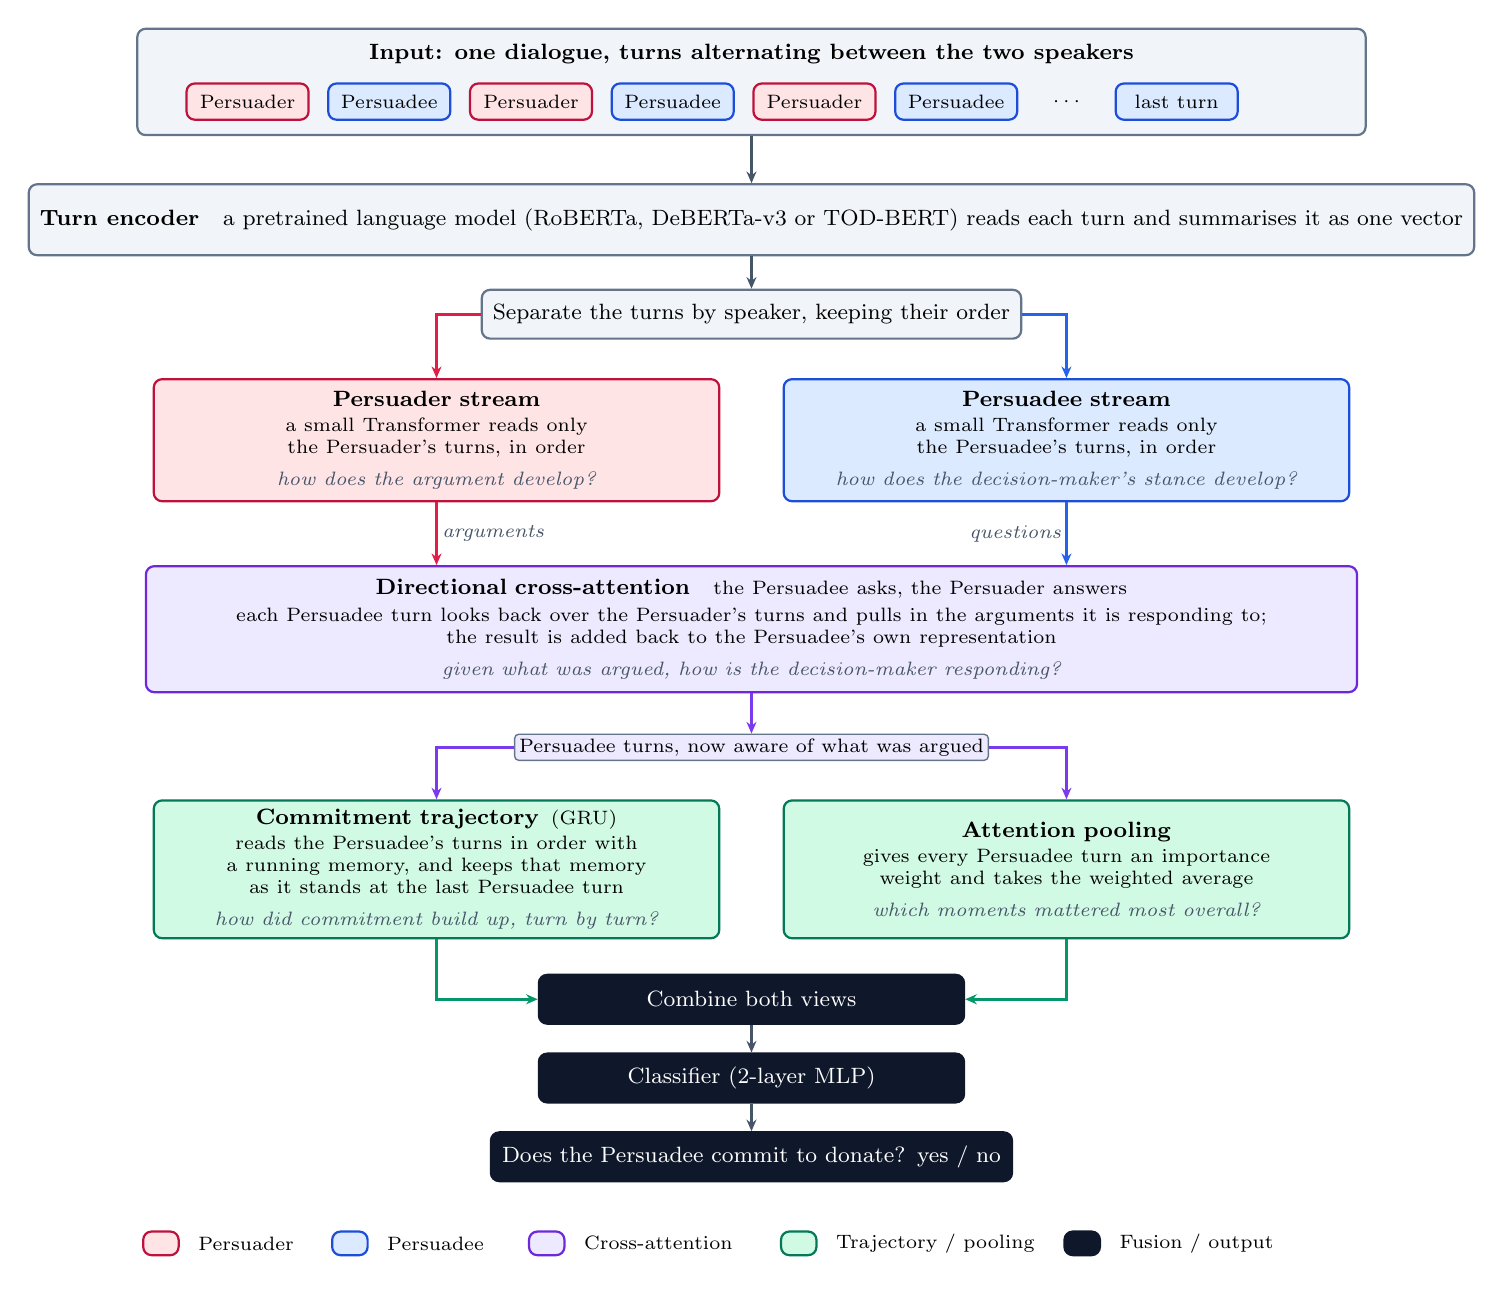
\begin{tikzpicture}[x=1cm,y=1cm,
  why/.style={font=\scriptsize\itshape},
  lbl/.style={font=\scriptsize\itshape, text=SlateSoft, fill=white, inner sep=1.5pt},
  chip/.style={minimum width=1.55cm, minimum height=0.46cm, inner sep=1pt, font=\scriptsize},
]

% ---------------- input dialogue ----------------------------------------------
\node[neu, minimum width=15.6cm, minimum height=1.35cm] (dlg) at (8,0) {};
\node[ttl] at (8,0.36) {Input: one dialogue, turns alternating between the two speakers};
\foreach \i/\x in {1/1.6,3/5.2,5/8.8}{
  \node[per, chip] at (\x,-0.25) {Persuader};}
\foreach \i/\x in {2/3.4,4/7.0,6/10.6}{
  \node[dec, chip] at (\x,-0.25) {Persuadee};}
\node[font=\scriptsize] at (12.0,-0.25) {$\cdots$};
\node[dec, chip] at (13.4,-0.25) {last turn};

% ---------------- turn encoder and split ------------------------------------------
\node[neu, minimum width=15.6cm, minimum height=0.9cm] (enc) at (8,-1.75)
  {\textbf{Turn encoder}\quad a pretrained language model (RoBERTa, DeBERTa-v3 or TOD-BERT) reads each turn and summarises it as one vector};
\draw[flow] (dlg) -- (enc);
\node[neu, minimum width=6.2cm] (split) at (8,-2.95) {Separate the turns by speaker, keeping their order};
\draw[flow] (enc) -- (split);

% ---------------- two speaker streams ---------------------------------------------
\node[per, text width=6.9cm, minimum height=1.55cm] (sP) at (4.0,-4.55)
  {\textbf{Persuader stream}\\[1pt]\scriptsize a small Transformer reads only the Persuader's turns, in order\\[2pt] {\scriptsize\itshape\color{SlateSoft} how does the argument develop?}};
\node[dec, text width=6.9cm, minimum height=1.55cm] (sD) at (12.0,-4.55)
  {\textbf{Persuadee stream}\\[1pt]\scriptsize a small Transformer reads only the Persuadee's turns, in order\\[2pt] {\scriptsize\itshape\color{SlateSoft} how does the decision-maker's stance develop?}};
\draw[flowP] (split.west) -| (sP.north);
\draw[flowD] (split.east) -| (sD.north);

% ---------------- directional cross-attention -------------------------------------
\node[xat, text width=15.1cm, minimum height=1.6cm] (xa) at (8,-6.95)
  {\textbf{Directional cross-attention}\quad{\scriptsize the Persuadee asks, the Persuader answers}\\[2pt]
   \scriptsize each Persuadee turn looks back over the Persuader's turns and pulls in the arguments it is responding to;\\
   \scriptsize the result is added back to the Persuadee's own representation\\[2pt]
   {\scriptsize\itshape\color{SlateSoft} given what was argued, how is the decision-maker responding?}};
\draw[flowP] (sP.south) -- node[lbl, right] {arguments} (sP.south |- xa.north);
\draw[flowD] (sD.south) -- node[lbl, left] {questions} (sD.south |- xa.north);

\node[ten, fill=XatFill, font=\scriptsize] (ctx) at (8,-8.45) {Persuadee turns, now aware of what was argued};
\draw[flowX] (xa) -- (ctx);

% ---------------- two readouts --------------------------------------------------
\node[trj, text width=6.9cm, minimum height=1.75cm] (gru) at (4.0,-10.0)
  {\textbf{Commitment trajectory}\enspace{\scriptsize(GRU)}\\[1pt]\scriptsize reads the Persuadee's turns in order with a running memory, and keeps that memory as it stands at the last Persuadee turn\\[2pt] {\scriptsize\itshape\color{SlateSoft} how did commitment build up, turn by turn?}};
\node[trj, text width=6.9cm, minimum height=1.75cm] (pool) at (12.0,-10.0)
  {\textbf{Attention pooling}\\[1pt]\scriptsize gives every Persuadee turn an importance weight and takes the weighted average\\[2pt] {\scriptsize\itshape\color{SlateSoft} which moments mattered most overall?}};
\draw[flowX] (ctx.west) -| (gru.north);
\draw[flowX] (ctx.east) -| (pool.north);

% ---------------- fusion, head, output --------------------------------------------
\node[fin, minimum width=5.4cm] (cat) at (8,-11.65) {Combine both views};
\draw[flowT] (gru.south) |- (cat.west);
\draw[flowT] (pool.south) |- (cat.east);
\node[fin, minimum width=5.4cm] (head) at (8,-12.65) {Classifier (2-layer MLP)};
\node[fin, minimum width=5.4cm] (yh) at (8,-13.65) {Does the Persuadee commit to donate?\enspace yes / no};
\draw[flow] (cat) -- (head); \draw[flow] (head) -- (yh);

% ---------------- legend ------------------------------------------------------------
\begin{scope}[shift={(0.5,-14.75)}]
  \node[per, minimum width=0.45cm, minimum height=0.3cm] at (0,0) {};
  \node[anchor=west, font=\scriptsize] at (0.35,0) {Persuader};
  \node[dec, minimum width=0.45cm, minimum height=0.3cm] at (2.4,0) {};
  \node[anchor=west, font=\scriptsize] at (2.75,0) {Persuadee};
  \node[xat, minimum width=0.45cm, minimum height=0.3cm] at (4.9,0) {};
  \node[anchor=west, font=\scriptsize] at (5.25,0) {Cross-attention};
  \node[trj, minimum width=0.45cm, minimum height=0.3cm] at (8.1,0) {};
  \node[anchor=west, font=\scriptsize] at (8.45,0) {Trajectory / pooling};
  \node[fin, minimum width=0.45cm, minimum height=0.3cm] at (11.7,0) {};
  \node[anchor=west, font=\scriptsize] at (12.05,0) {Fusion / output};
\end{scope}

\end{tikzpicture}
}
  \caption{High-level conceptual schematic of the AntiphonyClassifier architecture, illustrating the intuitive information flow from alternating conversational turns to speaker stream disentanglement, directional asymmetric cross-attention, dual trajectory and attention pooling context aggregation, and final commitment classification.}
  \label{fig:antiphony_simple}
\end{figure}

\subsection{Detailed Mathematical Formulation}
Let dialogue $\mathcal{D}$ comprise $U$ utterances ($U \le 32$), each truncated to $L=64$ tokens.
\begin{enumerate}
  \item \textbf{Batched Utterance Encoding:} The input tensor $\mathbf{X} \in \mathbb{R}^{B \times U \times L}$ is flattened to $[B \cdot U, L]$ and passed through a single batched forward pass of a shared transformer encoder (e.g., DeBERTa-v3-base), yielding token hidden states $\mathbf{E} \in \mathbb{R}^{(B \cdot U) \times L \times d}$ where $d=768$. Masked mean-pooling over valid non-padded tokens produces utterance vectors $\mathbf{U} \in \mathbb{R}^{B \times U \times d}$.
  \item \textbf{Role-Pure Disentanglement:} Utterances are partitioned using binary role masks into two role-pure streams: Persuader turns $\mathbf{H}^{(\mathcal{P})} \in \mathbb{R}^{B \times R_{\mathcal{P}} \times d}$ and Persuadee/Decider turns $\mathbf{H}^{(\mathcal{D})} \in \mathbb{R}^{B \times R_{\mathcal{D}} \times d}$, where each stream retains the last $R=20$ turns in chronological order with stream-local position embeddings.
  \item \textbf{Independent Stream Transformers:} Each stream is encoded by an independent 2-layer transformer with multi-head self-attention, pre-LayerNorm, and feed-forward sub-layers:
    \begin{equation}
      \widetilde{\mathbf{H}}^{(\mathcal{P})} = \text{Transformer}_{\mathcal{P}}(\mathbf{H}^{(\mathcal{P})}), \quad \widetilde{\mathbf{H}}^{(\mathcal{D})} = \text{Transformer}_{\mathcal{D}}(\mathbf{H}^{(\mathcal{D})})
    \end{equation}
  \item \textbf{Directional Asymmetric Cross-Attention:} To model how decider stance evolves in response to persuader arguments, the Decider stream acts as the Query, while the Persuader stream provides the Keys and Values:
    \begin{equation}
      \mathbf{Q} = \widetilde{\mathbf{H}}^{(\mathcal{D})} \mathbf{W}_Q, \quad \mathbf{K} = \widetilde{\mathbf{H}}^{(\mathcal{P})} \mathbf{W}_K, \quad \mathbf{V} = \widetilde{\mathbf{H}}^{(\mathcal{P})} \mathbf{W}_V
    \end{equation}
    \begin{equation}
      \mathbf{A}^{(\mathcal{D} \to \mathcal{P})} = \text{softmax}\left(\frac{\mathbf{Q} \mathbf{K}^\top}{\sqrt{d_k}} + \mathbf{M}_{\mathcal{P}}\right), \quad \mathbf{C}^{(\mathcal{D} \to \mathcal{P})} = \mathbf{A}^{(\mathcal{D} \to \mathcal{P})} \mathbf{V}
    \end{equation}
    The cross-attended representations are combined via residual layer normalization:
    \begin{equation}
      \mathbf{X} = \text{LayerNorm}(\widetilde{\mathbf{H}}^{(\mathcal{D})} + \mathbf{C}^{(\mathcal{D} \to \mathcal{P})})
    \end{equation}
  \item \textbf{Dual Context Aggregation:} The contextualized decider representations $\mathbf{X} = [\mathbf{x}_1, \dots, \mathbf{x}_T]$ are aggregated across two complementary paths:
    \begin{itemize}
      \item \textit{Commitment-Trajectory GRU:} Captures non-monotonic stance shifts via a recurrent hidden state:
        \begin{equation}
          \mathbf{h}_t = \text{GRU}(\mathbf{x}_t, \mathbf{h}_{t-1})
        \end{equation}
        The trajectory state $\mathbf{h}_T$ is extracted at the dialogue's true last valid decider turn, bypassing trailing padding slots.
      \item \textit{Learned Attention Pooling:} Computes an order-invariant summary of salient turns:
        \begin{equation}
          \alpha_t = \frac{\exp(\mathbf{w}_a^\top \tanh(\mathbf{W}_a \mathbf{x}_t))}{\sum_{j=1}^{T} \exp(\mathbf{w}_a^\top \tanh(\mathbf{W}_a \mathbf{x}_j))}, \quad \mathbf{p} = \sum_{t=1}^{T} \alpha_t \mathbf{x}_t
        \end{equation}
    \end{itemize}
  \item \textbf{Fusion and Classification Head:} The temporal trajectory vector $\mathbf{h}_T$ and the attention-pooled vector $\mathbf{p}$ are concatenated:
    \begin{equation}
      \mathbf{z} = [\mathbf{h}_T \,;\, \mathbf{p}] \in \mathbb{R}^{2d}
    \end{equation}
    and fed into a 2-layer MLP head ($\text{Linear}(2d, d) \to \text{GELU} \to \text{Dropout}(0.2) \to \text{Linear}(d, 2)$) producing unnormalized binary logits $\hat{\mathbf{y}} \in \mathbb{R}^2$.
  \item \textbf{Multi-Objective Training Loss:} Antiphony is optimized using a joint composite loss combining Class-Balanced Focal Loss \cite{cui2019class} ($\gamma=2.0, \beta=0.999$) and Supervised Contrastive Loss \cite{khosla2020supervised} ($\tau=0.1$, weight $\lambda_{\text{sc}} = 0.30$):
    \begin{equation}
      \mathcal{L} = \mathcal{L}_{\text{CB-Focal}}(\hat{\mathbf{y}}, y) + \lambda_{\text{sc}} \mathcal{L}_{\text{SupCon}}(\mathbf{z}, y)
    \end{equation}
\end{enumerate}

\begin{figure}[p]
  \centering
  \resizebox{\textwidth}{!}{% AntiphonyClassifier (v14): role-pure streams, directional cross-attention,
% commitment-trajectory GRU and parallel attention pooling.
% Drawn at 16 cm width; tensor names follow Section 4.6 of the report.
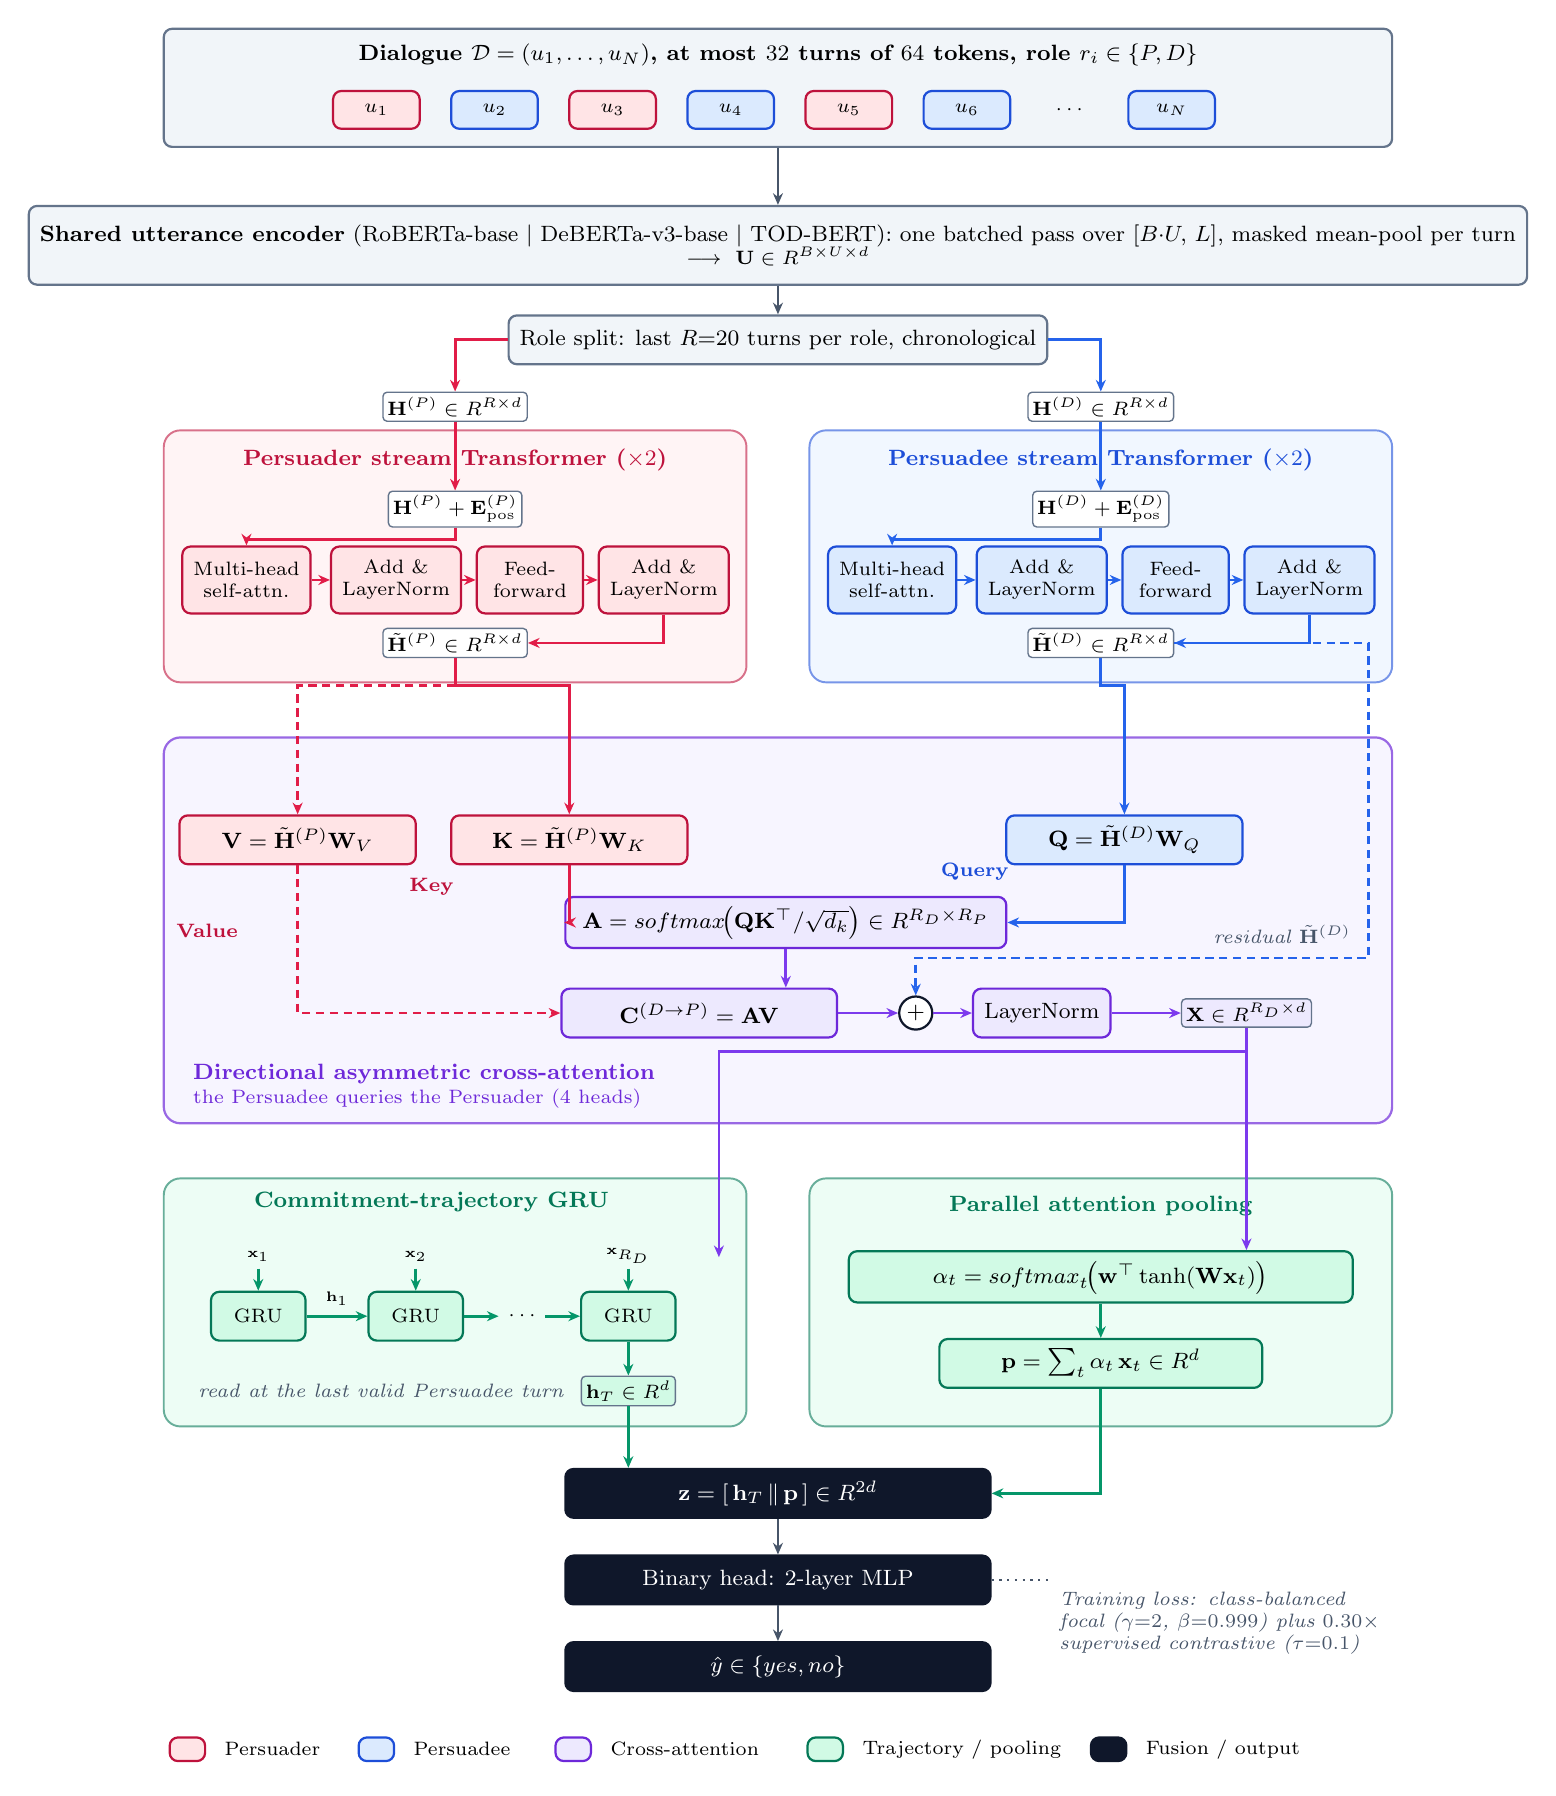
\begin{tikzpicture}[x=1cm,y=1cm]

% ---------------- group backdrops (drawn first, nodes sit on top) --------------
\draw[rounded corners=6pt, draw=PerBord!60, fill=PerFill!40, line width=0.7pt] (0.2,-4.35) rectangle (7.6,-7.55);
\draw[rounded corners=6pt, draw=DecBord!60, fill=DecFill!40, line width=0.7pt] (8.4,-4.35) rectangle (15.8,-7.55);
\draw[rounded corners=6pt, draw=XatBord!70, fill=XatFill!45, line width=0.8pt] (0.2,-8.25) rectangle (15.8,-13.15);
\draw[rounded corners=6pt, draw=TrjBord!60, fill=TrjFill!40, line width=0.7pt] (0.2,-13.85) rectangle (7.6,-17.0);
\draw[rounded corners=6pt, draw=TrjBord!60, fill=TrjFill!40, line width=0.7pt] (8.4,-13.85) rectangle (15.8,-17.0);

% ---------------- input dialogue ----------------------------------------------
\node[neu, minimum width=15.6cm, minimum height=1.5cm] (dlg) at (8,0) {};
\node[ttl] at (8,0.42) {Dialogue $\mathcal{D}=(u_1,\dots,u_N)$, at most $32$ turns of $64$ tokens, role $r_i\in\{P,D\}$};
\foreach \i [evaluate=\xx using {1.4+1.5*\i}] in {1,3,5}{
  \node[per, minimum width=1.1cm, minimum height=0.48cm, inner sep=1pt, font=\scriptsize] at (\xx,-0.28) {$u_{\i}$};}
\foreach \i [evaluate=\xx using {1.4+1.5*\i}] in {2,4,6}{
  \node[dec, minimum width=1.1cm, minimum height=0.48cm, inner sep=1pt, font=\scriptsize] at (\xx,-0.28) {$u_{\i}$};}
\node[font=\scriptsize] at (11.7,-0.28) {$\cdots$};
\node[dec, minimum width=1.1cm, minimum height=0.48cm, inner sep=1pt, font=\scriptsize] at (13.0,-0.28) {$u_N$};

% ---------------- shared utterance encoder ---------------------------------------
\node[neu, minimum width=15.6cm, minimum height=1.0cm] (enc) at (8,-2.0)
  {\textbf{Shared utterance encoder} (RoBERTa-base $\mid$ DeBERTa-v3-base $\mid$ TOD-BERT): one batched pass over $[B{\cdot}U,\,L]$, masked mean-pool per turn\\[-1pt]
   {\scriptsize $\longrightarrow\ \mathbf{U}\in\mathbb{R}^{B\times U\times d}$}};
\draw[flow] (dlg.south) -- (enc.north);

% ---------------- role split ------------------------------------------------------
\node[neu, minimum width=6.2cm] (split) at (8,-3.2) {Role split: last $R{=}20$ turns per role, chronological};
\draw[flow] (enc.south) -- (split.north);
\node[ten] (hP) at (3.9,-4.05) {$\mathbf{H}^{(P)}\in\mathbb{R}^{R\times d}$};
\node[ten] (hD) at (12.1,-4.05) {$\mathbf{H}^{(D)}\in\mathbb{R}^{R\times d}$};
\draw[flowP] (split.west) -| (hP.north);
\draw[flowD] (split.east) -| (hD.north);

% ---------------- stream transformers ---------------------------------------------
\node[ttl, text=PerBord] at (3.9,-4.72) {Persuader stream Transformer ($\times 2$)};
\node[ttl, text=DecBord] at (12.1,-4.72) {Persuadee stream Transformer ($\times 2$)};
\node[ten] (pP) at (3.9,-5.35) {$\mathbf{H}^{(P)}+\mathbf{E}^{(P)}_{\mathrm{pos}}$};
\node[ten] (pD) at (12.1,-5.35) {$\mathbf{H}^{(D)}+\mathbf{E}^{(D)}_{\mathrm{pos}}$};
% sub-layer chain, persuader
\node[per, minimum width=1.55cm, minimum height=0.85cm, font=\scriptsize] (aP1) at (1.25,-6.25) {Multi-head\\self-attn.};
\node[per, minimum width=1.35cm, minimum height=0.85cm, font=\scriptsize] (aP2) at (3.15,-6.25) {Add \&\\LayerNorm};
\node[per, minimum width=1.35cm, minimum height=0.85cm, font=\scriptsize] (aP3) at (4.85,-6.25) {Feed-\\forward};
\node[per, minimum width=1.35cm, minimum height=0.85cm, font=\scriptsize] (aP4) at (6.55,-6.25) {Add \&\\LayerNorm};
\draw[flowP] (pP.south) -- ++(0,-0.15) -| (aP1.north);
\draw[flowP] (aP1) -- (aP2); \draw[flowP] (aP2) -- (aP3); \draw[flowP] (aP3) -- (aP4);
% sub-layer chain, persuadee
\node[dec, minimum width=1.55cm, minimum height=0.85cm, font=\scriptsize] (aD1) at (9.45,-6.25) {Multi-head\\self-attn.};
\node[dec, minimum width=1.35cm, minimum height=0.85cm, font=\scriptsize] (aD2) at (11.35,-6.25) {Add \&\\LayerNorm};
\node[dec, minimum width=1.35cm, minimum height=0.85cm, font=\scriptsize] (aD3) at (13.05,-6.25) {Feed-\\forward};
\node[dec, minimum width=1.35cm, minimum height=0.85cm, font=\scriptsize] (aD4) at (14.75,-6.25) {Add \&\\LayerNorm};
\draw[flowD] (pD.south) -- ++(0,-0.15) -| (aD1.north);
\draw[flowD] (aD1) -- (aD2); \draw[flowD] (aD2) -- (aD3); \draw[flowD] (aD3) -- (aD4);
% split -> stream inputs
\draw[flowP] (hP.south) -- (pP.north);
\draw[flowD] (hD.south) -- (pD.north);
% outputs of the streams
\node[ten] (tP) at (3.9,-7.05) {$\tilde{\mathbf{H}}^{(P)}\in\mathbb{R}^{R\times d}$};
\node[ten] (tD) at (12.1,-7.05) {$\tilde{\mathbf{H}}^{(D)}\in\mathbb{R}^{R\times d}$};
\draw[flowP] (aP4.south) |- (tP.east);
\draw[flowD] (aD4.south) |- (tD.east);

% ---------------- cross-attention block -------------------------------------------
\node[ttl, text=XatBord, anchor=west, align=left] at (0.45,-12.68) {Directional asymmetric cross-attention\\[-1pt]{\scriptsize\normalfont the Persuadee queries the Persuader ($4$ heads)}};
\node[per, minimum width=3.0cm] (wV) at (1.9,-9.55) {$\mathbf{V}=\tilde{\mathbf{H}}^{(P)}\mathbf{W}_V$};
\node[per, minimum width=3.0cm] (wK) at (5.35,-9.55) {$\mathbf{K}=\tilde{\mathbf{H}}^{(P)}\mathbf{W}_K$};
\node[dec, minimum width=3.0cm] (wQ) at (12.4,-9.55) {$\mathbf{Q}=\tilde{\mathbf{H}}^{(D)}\mathbf{W}_Q$};
\draw[flowP] (tP.south) -- ++(0,-0.35) -| (wK.north);
\draw[flowP, dsh] (tP.south) -- ++(0,-0.35) -| (wV.north);
\draw[flowD] (tD.south) -- ++(0,-0.35) -| (wQ.north);

\node[xat, minimum width=5.6cm] (att) at (8.1,-10.6)
  {$\mathbf{A}=\operatorname{softmax}\!\big(\mathbf{Q}\mathbf{K}^{\top}/\sqrt{d_k}\big)\in\mathbb{R}^{R_D\times R_P}$};
\draw[flowP] (wK.south) |- (att.west);
\draw[flowD] (wQ.south) |- (att.east);
\node[xat, minimum width=3.5cm] (cv) at (7.0,-11.75) {$\mathbf{C}^{(D\to P)}=\mathbf{A}\mathbf{V}$};
\draw[flowX] (att.south) -- (att.south |- cv.north);
\draw[flowP, dsh] (wV.south) |- (cv.west);
\node[oplus] (ad) at (9.75,-11.75) {$+$};
\node[xat, minimum width=1.7cm] (ln) at (11.35,-11.75) {LayerNorm};
\node[ten, fill=XatFill] (xx) at (13.95,-11.75) {$\mathbf{X}\in\mathbb{R}^{R_D\times d}$};
\draw[flowX] (cv) -- (ad);
\draw[flowX] (ad) -- (ln);
\draw[flowX] (ln) -- (xx);
% residual from the Persuadee stream
\draw[flowD, dsh] (tD.east) -- (15.5,-7.05) -- (15.5,-11.05) -- (9.75,-11.05) -- (ad.north);
\node[nt,anchor=east] at (15.4,-10.75) {residual $\tilde{\mathbf{H}}^{(D)}$};
\node[font=\scriptsize\bfseries, text=DecBord] at (10.5,-9.95) {Query};
\node[font=\scriptsize\bfseries, text=PerBord] at (3.6,-10.15) {Key};
\node[font=\scriptsize\bfseries, text=PerBord] at (0.75,-10.7) {Value};

% ---------------- dual aggregation ------------------------------------------------
\draw[flowX] (xx.south) -- ++(0,-0.3) -| (7.25,-14.85);
\node[ttl, text=TrjBord] at (3.6,-14.15) {Commitment-trajectory GRU};
\node[trj, minimum width=1.2cm, font=\scriptsize] (g1) at (1.4,-15.6) {GRU};
\node[trj, minimum width=1.2cm, font=\scriptsize] (g2) at (3.4,-15.6) {GRU};
\node[font=\scriptsize] (gd) at (4.75,-15.6) {$\cdots$};
\node[trj, minimum width=1.2cm, font=\scriptsize] (g3) at (6.1,-15.6) {GRU};
\draw[flowT] (g1) -- node[above,font=\tiny]{$\mathbf{h}_1$} (g2);
\draw[flowT] (g2) -- (gd); \draw[flowT] (gd) -- (g3);
\foreach \g/\l in {g1/{\mathbf{x}_1},g2/{\mathbf{x}_2},g3/{\mathbf{x}_{R_D}}}{
  \draw[flowT] ([yshift=0.28cm]\g.north) -- (\g.north); \node[font=\tiny] at ([yshift=0.44cm]\g.north) {$\l$};}
\node[ten, fill=TrjFill] (hT) at (6.1,-16.55) {$\mathbf{h}_T\in\mathbb{R}^{d}$};
\draw[flowT] (g3.south) -- (hT.north);
\node[nt,anchor=east] at (5.4,-16.55) {read at the last valid Persuadee turn};

\node[ttl, text=TrjBord] at (12.1,-14.2) {Parallel attention pooling};
\node[trj, minimum width=6.4cm] (alph) at (12.1,-15.1) {$\alpha_t=\operatorname{softmax}_t\!\big(\mathbf{w}^{\top}\tanh(\mathbf{W}\mathbf{x}_t)\big)$};
\node[trj, minimum width=4.1cm] (pv) at (12.1,-16.2) {$\mathbf{p}=\sum_{t}\alpha_t\,\mathbf{x}_t\in\mathbb{R}^{d}$};
\draw[flowT] (alph) -- (pv);
\draw[flowX] (xx.south) -- (xx.south |- alph.north);

% ---------------- fusion, head, output --------------------------------------------
\node[fin,minimum width=5.4cm] (cat) at (8,-17.85) {$\mathbf{z}=[\,\mathbf{h}_T\,\Vert\,\mathbf{p}\,]\in\mathbb{R}^{2d}$};
\draw[flowT] (hT.south) -- (hT.south |- cat.north);
\draw[flowT] (pv.south) |- (cat.east);
\node[fin,minimum width=5.4cm] (head) at (8,-18.95) {Binary head: 2-layer MLP};
\node[fin,minimum width=5.4cm] (yh) at (8,-20.05) {$\hat{y}\in\{\text{yes},\text{no}\}$};
\draw[flow] (cat) -- (head); \draw[flow] (head) -- (yh);
\node[nt,anchor=west, text width=4.4cm, align=left] (lossnote) at (11.45,-19.5)
  {Training loss: class-balanced focal ($\gamma{=}2$, $\beta{=}0.999$) plus $0.30\times$ supervised contrastive ($\tau{=}0.1$)};
\draw[dotted, line width=0.8pt, draw=SlateSoft] (head.east) -- (head.east -| lossnote.west) -- (lossnote.north west);

% ---------------- legend ------------------------------------------------------------
\begin{scope}[shift={(0.5,-21.1)}]
  \node[per, minimum width=0.45cm, minimum height=0.3cm] (l1) at (0,0) {};
  \node[anchor=west, font=\scriptsize] at (0.35,0) {Persuader};
  \node[dec, minimum width=0.45cm, minimum height=0.3cm] at (2.4,0) {};
  \node[anchor=west, font=\scriptsize] at (2.75,0) {Persuadee};
  \node[xat, minimum width=0.45cm, minimum height=0.3cm] at (4.9,0) {};
  \node[anchor=west, font=\scriptsize] at (5.25,0) {Cross-attention};
  \node[trj, minimum width=0.45cm, minimum height=0.3cm] at (8.1,0) {};
  \node[anchor=west, font=\scriptsize] at (8.45,0) {Trajectory / pooling};
  \node[fin,minimum width=0.45cm, minimum height=0.3cm] at (11.7,0) {};
  \node[anchor=west, font=\scriptsize] at (12.05,0) {Fusion / output};
\end{scope}

\end{tikzpicture}
}
  \caption{Detailed neural architecture and tensor specifications of the AntiphonyClassifier, depicting exact layer dimensions, 2-layer independent stream Transformers, directional cross-attention ($\mathbf{Q}_{\mathcal{D}} \mathbf{K}_{\mathcal{P}}^\top / \sqrt{d_k}$), parallel commitment-trajectory GRU and learned attention pooling, and composite Class-Balanced Focal and Supervised Contrastive loss heads.}
  \label{fig:antiphony_arch}
\end{figure}

\begin{summarybox}[Directional Cross-Attention and Trajectory Invariant]
In the \textit{AntiphonyClassifier}, asymmetric conversational roles are embedded directly into the neural wiring:
\begin{equation}
  \mathbf{A}^{(\mathcal{D} \to \mathcal{P})} = \text{softmax}\left(\frac{\mathbf{Q}_{\mathcal{D}} \mathbf{K}_{\mathcal{P}}^\top}{\sqrt{d_k}} + \mathbf{M}_{\mathcal{P}}\right), \quad \mathbf{C}^{(\mathcal{D} \to \mathcal{P})} = \mathbf{A}^{(\mathcal{D} \to \mathcal{P})} \mathbf{V}_{\mathcal{P}}
\end{equation}
The decider query $\mathbf{Q}_{\mathcal{D}}$ selectively attends to the persuader's rhetorical tactics $\mathbf{K}_{\mathcal{P}}, \mathbf{V}_{\mathcal{P}}$, updating the commitment-trajectory state $\mathbf{h}_t = \text{GRU}(\mathbf{x}_t, \mathbf{h}_{t-1})$ read strictly at the dialogue's true final decider turn. This architectural design ensures the model tracks temporal decision momentum while completely ignoring trailing post-decision pleasantries.
\end{summarybox}

\clearpage
\section{Architectural Evolution: The Path to Dual-Stream Antiphony}
\label{sec:evolution}

The AntiphonyClassifier was not designed in isolation; it emerged from a systematic multi-stage empirical investigation across four distinct evolutionary phases, documented in \Cref{fig:architectural_evolution}. This section refers to the deciding party by its dataset role, \emph{Persuadee}, the same participant termed \emph{Decider} in the architecture description of \Cref{sec:antiphony}.

\begin{figure}[htbp]
  \centering
  \resizebox{\textwidth}{!}{% Four architectural stages, v1 to v14. Metrics are the best test macro-F1 of each stage
% (Tables A and B of the report, 153-row test split).
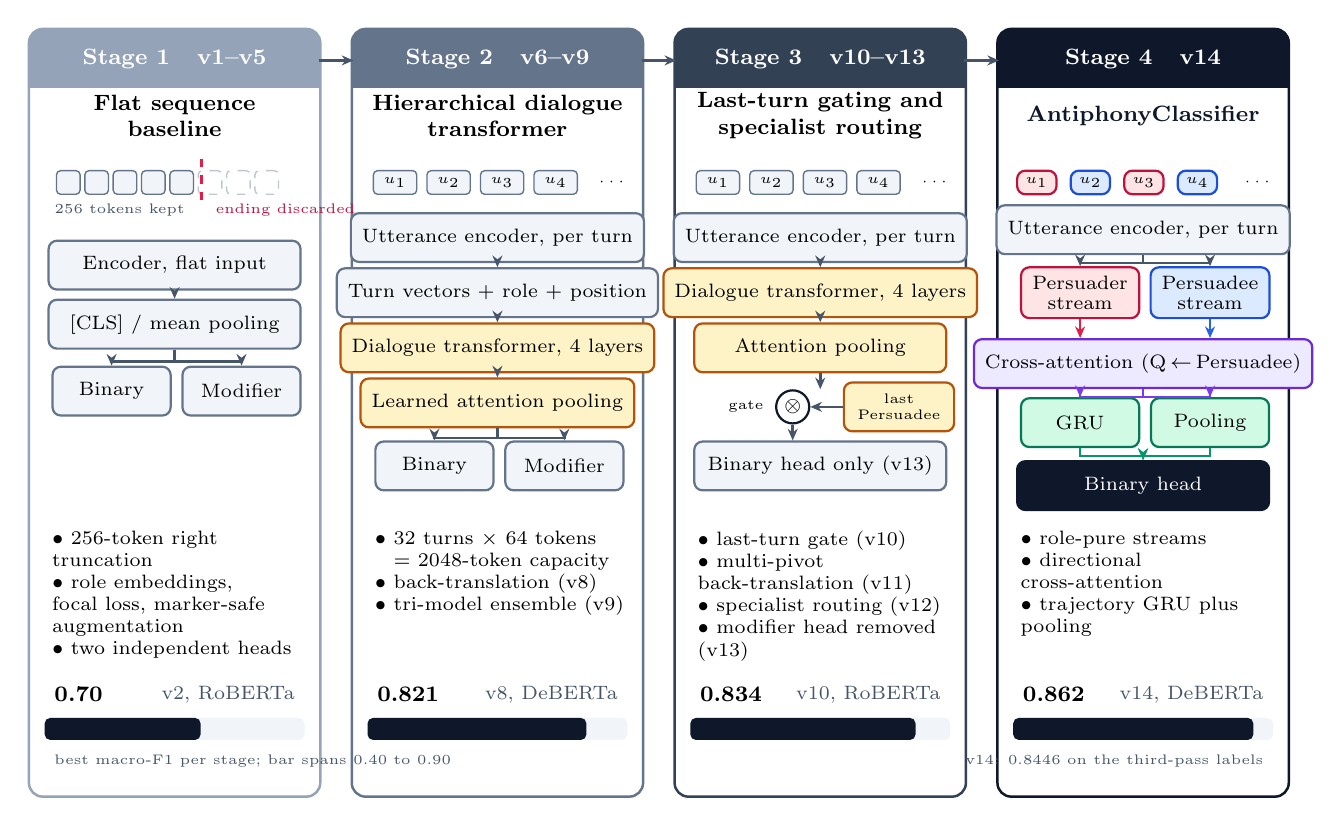
\begin{tikzpicture}[x=1cm,y=1cm]

% ------------- card frames and headers ---------------------------------------
\foreach \x/\c/\t in {0/94A3B8/{Stage 1\quad v1--v5}, 4.1/64748B/{Stage 2\quad v6--v9}, 8.2/334155/{Stage 3\quad v10--v13}, 12.3/0F172A/{Stage 4\quad v14}}{
  \definecolor{stg}{HTML}{\c}
  \draw[rounded corners=5pt, draw=stg, fill=white, line width=0.9pt] (\x,0.05) rectangle ++(3.7,-9.75);
  \fill[stg, rounded corners=5pt] (\x,0.05) rectangle ++(3.7,-0.75);
  \fill[stg] (\x,-0.4) rectangle ++(3.7,-0.3);
  \node[text=white, font=\footnotesize\bfseries] at (\x+1.85,-0.33) {\t};
}
\foreach \x in {3.7,7.8,11.9}{ \draw[flow, line width=1.3pt] (\x-0.02,-0.35) -- ++(0.44,0); }

% ------------- titles -----------------------------------------------------------
\node[ttl] at (1.85,-1.05) {Flat sequence\\baseline};
\node[ttl] at (5.95,-1.05) {Hierarchical dialogue\\transformer};
\node[ttl] at (10.05,-1.05) {Last-turn gating and\\specialist routing};
\node[ttl, text=Slate] at (14.15,-1.05) {AntiphonyClassifier};

% =============== Stage 1 : flat baseline ========================================
\begin{scope}[shift={(0,0)}]
  \foreach \i in {0,1,2,3,4}{ \node[ten, minimum size=0.3cm, fill=NeuFill] at (0.5+0.36*\i,-1.9) {}; }
  \foreach \i in {5,6,7}{ \node[ten, minimum size=0.3cm, draw=NeuBord!40, dashed, text=NeuBord!40] at (0.5+0.36*\i,-1.9) {}; }
  \draw[PerMain, dashed, line width=0.9pt] (2.19,-1.6) -- (2.19,-2.2);
  \node[font=\tiny, text=PerBord, anchor=west] at (2.25,-2.25) {ending discarded};
  \node[font=\tiny, text=SlateSoft, anchor=east] at (2.1,-2.25) {256 tokens kept};
  \node[neu, minimum width=3.2cm] (e1) at (1.85,-2.95) {\scriptsize Encoder, flat input};
  \node[neu, minimum width=3.2cm] (p1) at (1.85,-3.7) {\scriptsize {[}CLS{]} / mean pooling};
  \node[neu, minimum width=1.5cm] (h1a) at (1.05,-4.55) {\scriptsize Binary};
  \node[neu, minimum width=1.5cm] (h1b) at (2.7,-4.55) {\scriptsize Modifier};
  \draw[flow] (e1) -- (p1);
  \draw[flow] (p1.south) -- ++(0,-0.15) -| (h1a.north);
  \draw[flow] (p1.south) -- ++(0,-0.15) -| (h1b.north);
\end{scope}

% =============== Stage 2 : hierarchical =========================================
\begin{scope}[shift={(4.1,0)}]
  \foreach \i [evaluate=\j using {int(\i+1)}] in {0,1,2,3}{ \node[ten, minimum width=0.55cm, minimum height=0.3cm, fill=NeuFill] at (0.55+0.68*\i,-1.9) {\tiny $u_{\j}$}; }
  \node[font=\tiny] at (3.3,-1.9) {$\cdots$};
  \node[neu, minimum width=3.2cm] (e2) at (1.85,-2.6) {\scriptsize Utterance encoder, per turn};
  \node[neu, minimum width=3.2cm] (p2) at (1.85,-3.3) {\scriptsize Turn vectors + role + position};
  \node[amb, minimum width=3.2cm] (d2) at (1.85,-4.0) {\scriptsize Dialogue transformer, 4 layers};
  \node[amb, minimum width=3.2cm] (a2) at (1.85,-4.7) {\scriptsize Learned attention pooling};
  \node[neu, minimum width=1.5cm] (h2a) at (1.05,-5.5) {\scriptsize Binary};
  \node[neu, minimum width=1.5cm] (h2b) at (2.7,-5.5) {\scriptsize Modifier};
  \draw[flow] (e2) -- (p2); \draw[flow] (p2) -- (d2); \draw[flow] (d2) -- (a2);
  \draw[flow] (a2.south) -- ++(0,-0.12) -| (h2a.north);
  \draw[flow] (a2.south) -- ++(0,-0.12) -| (h2b.north);
\end{scope}

% =============== Stage 3 : gating and routing ===================================
\begin{scope}[shift={(8.2,0)}]
  \foreach \i [evaluate=\j using {int(\i+1)}] in {0,1,2,3}{ \node[ten, minimum width=0.55cm, minimum height=0.3cm, fill=NeuFill] at (0.55+0.68*\i,-1.9) {\tiny $u_{\j}$}; }
  \node[font=\tiny] at (3.3,-1.9) {$\cdots$};
  \node[neu, minimum width=3.2cm] (e3) at (1.85,-2.6) {\scriptsize Utterance encoder, per turn};
  \node[amb, minimum width=3.2cm] (d3) at (1.85,-3.3) {\scriptsize Dialogue transformer, 4 layers};
  \node[amb, minimum width=3.2cm] (a3) at (1.85,-4.0) {\scriptsize Attention pooling};
  \node[oplus] (g3) at (1.5,-4.75) {\scriptsize $\otimes$};
  \node[amb, minimum width=1.4cm, font=\tiny] (l3) at (2.85,-4.75) {last\\Persuadee};
  \node[font=\tiny, anchor=east] at (1.25,-4.75) {gate};
  \node[neu, minimum width=3.2cm] (h3) at (1.85,-5.5) {\scriptsize Binary head only (v13)};
  \draw[flow] (e3) -- (d3); \draw[flow] (d3) -- (a3); \draw[flow] (a3.south) -- (a3.south |- g3.north); \draw[flow] (g3.south) -- (g3.south |- h3.north);
  \draw[flow] (l3.west) -- (g3.east);
\end{scope}

% =============== Stage 4 : Antiphony ============================================
\begin{scope}[shift={(12.3,0)}]
  \foreach \i [evaluate=\j using {int(\i+1)}] in {0,2}{ \node[per, minimum width=0.5cm, minimum height=0.3cm, inner sep=0pt, font=\tiny] at (0.5+0.68*\i,-1.9) {$u_{\j}$}; }
  \foreach \i [evaluate=\j using {int(\i+1)}] in {1,3}{ \node[dec, minimum width=0.5cm, minimum height=0.3cm, inner sep=0pt, font=\tiny] at (0.5+0.68*\i,-1.9) {$u_{\j}$}; }
  \node[font=\tiny] at (3.3,-1.9) {$\cdots$};
  \node[neu, minimum width=3.2cm] (e4) at (1.85,-2.5) {\scriptsize Utterance encoder, per turn};
  \node[per, minimum width=1.5cm] (sp) at (1.05,-3.3) {\scriptsize Persuader\\[-2pt]\scriptsize stream};
  \node[dec, minimum width=1.5cm] (sd) at (2.7,-3.3) {\scriptsize Persuadee\\[-2pt]\scriptsize stream};
  \node[xat, minimum width=3.2cm] (cx) at (1.85,-4.2) {\scriptsize Cross-attention (Q\,$\leftarrow$\,Persuadee)};
  \node[trj, minimum width=1.5cm] (gr) at (1.05,-4.95) {\scriptsize GRU};
  \node[trj, minimum width=1.5cm] (pl) at (2.7,-4.95) {\scriptsize Pooling};
  \node[fin, minimum width=3.2cm] (h4) at (1.85,-5.75) {\scriptsize Binary head};
  \draw[flow] (e4.south) -- ++(0,-0.1) -| (sp.north);
  \draw[flow] (e4.south) -- ++(0,-0.1) -| (sd.north);
  \draw[flowP] (sp.south) -- (sp.south |- cx.north);
  \draw[flowD] (sd.south) -- (sd.south |- cx.north);
  \draw[flowX] (cx.south) -- ++(0,-0.1) -| (gr.north);
  \draw[flowX] (cx.south) -- ++(0,-0.1) -| (pl.north);
  \draw[flowT] (gr.south) -- ++(0,-0.1) -| (h4.north);
  \draw[flowT] (pl.south) -- ++(0,-0.1) -| (h4.north);
\end{scope}

% ------------- what changed -------------------------------------------------------
\node[anchor=north west, text width=3.35cm, font=\scriptsize, align=left] at (0.17,-6.2)
  {$\bullet$ 256-token right truncation\\
   $\bullet$ role embeddings, focal loss, marker-safe augmentation\\
   $\bullet$ two independent heads};
\node[anchor=north west, text width=3.35cm, font=\scriptsize, align=left] at (4.27,-6.2)
  {$\bullet$ 32 turns $\times$ 64 tokens\\ \hphantom{$\bullet$} = 2048-token capacity\\
   $\bullet$ back-translation (v8)\\
   $\bullet$ tri-model ensemble (v9)};
\node[anchor=north west, text width=3.35cm, font=\scriptsize, align=left] at (8.37,-6.2)
  {$\bullet$ last-turn gate (v10)\\
   $\bullet$ multi-pivot back-translation (v11)\\
   $\bullet$ specialist routing (v12)\\
   $\bullet$ modifier head removed (v13)};
\node[anchor=north west, text width=3.35cm, font=\scriptsize, align=left] at (12.47,-6.2)
  {$\bullet$ role-pure streams\\
   $\bullet$ directional cross-attention\\
   $\bullet$ trajectory GRU plus pooling};

% ------------- performance bars ----------------------------------------------------
% track = 3.3 cm spans macro-F1 0.40 to 0.90
\foreach \x/\v/\w/\lab/\sub in {0.2/0.70/1.98/0.70/{v2, RoBERTa},
                                4.3/0.821/2.78/0.821/{v8, DeBERTa},
                                8.4/0.834/2.86/0.834/{v10, RoBERTa},
                                12.5/0.862/3.05/0.862/{v14, DeBERTa}}{
  \fill[NeuFill, rounded corners=2pt] (\x,-8.7) rectangle ++(3.3,-0.28);
  \fill[Slate, rounded corners=2pt] (\x,-8.7) rectangle ++(\w,-0.28);
  \node[font=\footnotesize\bfseries, anchor=west] at (\x,-8.4) {\lab};
  \node[font=\scriptsize, anchor=east, text=SlateSoft] at (\x+3.3,-8.4) {\sub};
}
\node[font=\tiny, text=SlateSoft, anchor=north west] at (0.2,-9.05) {best macro-F1 per stage; bar spans 0.40 to 0.90};
\node[font=\tiny, text=SlateSoft, anchor=north east] at (15.8,-9.05) {v14: 0.8446 on the third-pass labels};

\end{tikzpicture}
}
  \caption{Four-stage architectural evolution of intention classification models, depicting key innovations, critical bug diagnoses, and peak test Macro-F1 across stages.}
  \label{fig:architectural_evolution}
\end{figure}

\subsection{Stage 1: Monolithic Flat Baselines and Forensic Debugging}
\begin{itemize}
  \item \textbf{Flat Sequence Base Model (M1):} Concatenated dialogues truncated to 256 tokens with \texttt{[CLS]} pooling and independent binary and modifier heads. Reached $0.68$ Macro-F1 with RoBERTa, but DeBERTa skewed heavily toward the majority class (Macro-F1 $0.53$, only modestly above the $0.42$ majority-baseline) and modifier heads completely failed on rare classes.
  \item \textbf{Speaker-Aware Flat Encoding (M2):} Added learnable role embeddings ($\text{Persuader}=0, \text{Persuadee}=1$) prior to masked mean-pooling. Binary Macro-F1 rose to $0.70$ (RoBERTa) and recall on the rare \texttt{deferred} modifier class improved, but overall performance remained bottlenecked by 256-token truncation.
  \item \textbf{Dynamic Augmentation Exploration (M3):} Added EDA text augmentation \cite{wei2019eda} and raw inverse-frequency class weighting. Training completely collapsed. Forensic auditing identified two critical bugs: (i) checkpoint selection was mistakenly scored on \texttt{pos\_label="yes"} F1, allowing an all-yes trivial model to score $1.0$ and be saved, and (ii) raw inverse-frequency weights on the 13-example \texttt{conditional} class caused catastrophic gradient spikes.
  \item \textbf{Metric-Corrected Focal Loss Baseline (M4):} Fixed the evaluation harness to use true unweighted Macro-F1; implemented Class-Balanced Focal Loss ($\beta=0.999$); cascaded the binary prediction into the modifier head; added in-batch Supervised Contrastive Loss. Training stabilized, but performance plateaued at $0.649$ Macro-F1 (RoBERTa and TOD-BERT; DeBERTa $0.630$).
  \item \textbf{Token-Safe Augmentation Audit (M5):} An audit revealed that $57.5\%$ of speaker markers (\texttt{[Persuader]}) in raw transcripts were glued to newlines without spaces. Standard whitespace augmentation tokenizers fragmented these tags, corrupting role markers in $15.9\%$ of augmented instances. Implementing regex-based tokenization and Persuadee-biased mutation weights resolved the corruption, but Macro-F1 for DeBERTa remained capped at $0.670$, still short of M2's $0.70$ RoBERTa result; no backbone in this flat, 256-token family ever exceeded that RoBERTa figure, motivating the architectural change in Stage 2.
\end{itemize}

\subsection{Stage 2: Hierarchical Discourse Modeling}
\begin{itemize}
  \item \textbf{Hierarchical Dialogue Transformer (M6):} The foundational breakthrough: turns encoded individually ($32 \times 64 = 2{,}048$ token capacity) via a shared encoder, pooled into turn vectors, combined with role and positional embeddings, and processed by a 4-layer inter-turn dialogue transformer with learned attention pooling. Macro-F1 surged to \textbf{$0.793$} (RoBERTa), \textbf{$0.797$} (DeBERTa), and \textbf{$0.807$} (TOD-BERT).
  \item \textbf{Flat Back-Translation Control (M7):} Applied French back-translation to the flat M5 model as an experimental control; Macro-F1 dropped to $0.590$--$0.650$, proving that data augmentation cannot overcome architectural truncation.
  \item \textbf{Hierarchical Back-Translation (M8):} Combined the M6 hierarchical architecture with back-translation. Binary Macro-F1 advanced to \textbf{$0.821$} (DeBERTa), but modifier F1 fell, revealing that translation round-trips wash away subtle hedge words.
  \item \textbf{Tri-Model Soft Ensemble (M9):} Soft probability averaging across saved M6 checkpoints (RoBERTa, DeBERTa, TOD-BERT) achieved $0.818$ Macro-F1. 20 stochastic Monte Carlo dropout forward passes demonstrated that prediction variance was significantly lower on correct instances ($0.0220$) than incorrect instances ($0.0297$), providing a calibrated uncertainty signal.
\end{itemize}

\subsection{Stage 3: Recency Gating and Decoupled Baselines}
\begin{itemize}
  \item \textbf{Last-Persuadee-Turn Gating (M10):} Added a sigmoid gate explicitly anchoring the pooled representation to the final Persuadee hidden state, initialized with a $+3.0$ bias to prevent early deflection. Achieved \textbf{$0.834$} Macro-F1 with RoBERTa, establishing the peak single-model binary score of the two-headed lineage.
  \item \textbf{Multi-Pivot Back-Translation Diversity (M11):} Implemented French and German back-translation under beam search and random sampling; DeBERTa reached \textbf{$0.829$}, but modifier F1 continued to degrade.
  \item \textbf{Specialist Confidence Router (M12):} Decoupled the tasks without retraining: routing binary classification to M10 Gated RoBERTa ($0.834$) and modifier classification to M6 Plain DeBERTa ($0.452$).
  \item \textbf{Decoupled Single-Stream Baseline (M13):} Deleted the modifier head entirely, dedicating all capacity to a 2-layer binary head. Reached \textbf{$0.825$} on second-pass labels (RoBERTa); on third-pass labels, RoBERTa's default-threshold Macro-F1 is \textbf{$0.8359$}, marginally above its own tuned-threshold figure of $0.8290$ used as this model's officially reported result elsewhere in this report.
\end{itemize}

\subsection{Stage 4: Role-Pure Dual-Stream Antiphony Architecture}
The Dual-Stream Antiphony architecture (M14) implemented speaker-disentangled cross-attention, establishing project-wide peak performance: $0.8623$ Macro-F1 with DeBERTa at its default decision threshold on the second-pass benchmark ($0.8600$ under the tuned-threshold rule applied consistently to the other backbones on this benchmark), and $0.8446$ with RoBERTa at a tuned threshold on the strict third-pass benchmark, the shipped final model. These results definitively demonstrate the necessity of modeling asymmetric conversational dynamics.

\section{Design Refinement and Simulation}
\label{sec:detailed-design}

\subsection{Capacity Calculations and Sequence Length Budgeting}
In conversational modeling, sequence capacity must balance linguistic coverage against quadratic attention memory scaling ($\mathcal{O}(N^2)$). In the P4G corpus, dialogue length exhibits a median of 344 words across an average of 20 turns, with the 95th percentile reaching 23 turns. Flat transformers capped at 256 tokens cover fewer than 180 words, truncating over $50\%$ of conversational content. 

In Antiphony, the sequence budget allocates $U=32$ turns with $L=64$ tokens per turn, providing a total token capacity of:
\begin{equation}
  C_{\text{tokens}} = 32 \times 64 = 2{,}048 \text{ tokens}
\end{equation}
This budget covers $99.7\%$ of all conversational tokens across the corpus without truncation. For role-pure streams, setting $R=20$ turns per role provides capacity for up to 40 total turns, covering $98.8\%$ of dialogue trajectories.

\subsection{Memory Profiling and Hardware Guards}
Processing a batch of size $B$ with $U$ turns of length $L$ through a 768-dimensional transformer requires flattening to $[B \cdot U, L]$. For $B=4$ and $U=32$, this requires encoding 128 sequences of length 64 in a single forward pass. On an NVIDIA Tesla T4 GPU (16\,GB VRAM), peak activation memory for DeBERTa-v3 under standard precision exceeds hardware limits. We implemented three strict hardware guards:
\begin{enumerate}
  \item \textbf{Micro-Batch Slicing:} Training batch size is set to $B=2$, with evaluation batch size $B=4$.
  \item \textbf{Gradient Checkpointing:} Intermediate activation maps are discarded during the forward pass and recomputed during backpropagation, reducing activation memory by $\approx 60\%$.
  \item \textbf{PyTorch Dynamic Memory Allocation:} Enabled \texttt{expandable\_segments:True} in the PyTorch CUDA allocator to eliminate memory fragmentation during variable-length sequence packing.
\end{enumerate}

\section{Application of Tools}
\label{sec:tools}

The project utilized a cohesive suite of specialized computational tools:
\begin{itemize}
  \item \textbf{PyTorch 2.x \cite{paszke2019pytorch}:} Provided core automatic differentiation, custom CUDA autograd layers, and modular neural network implementations.
  \item \textbf{Hugging Face Transformers \cite{wolf2020transformers}:} Supplied pre-trained transformer backbones (RoBERTa, DeBERTa-v3, TOD-BERT, ELECTRA) and tokenization engines.
  \item \textbf{XGBoost \cite{chen2016xgboost} and Scikit-Learn:} Utilized for classical baseline construction, tabular stacking experiments, calibration curve fitting, and bootstrap evaluation metrics.
  \item \textbf{OPUS-MT \cite{tiedemann2020opusmt}:} Integrated for multilingual back-translation pipelines across French and German pivots.
  \item \textbf{Anthropic Claude 5 Sonnet:} Utilized as the automated frontier LLM rater for contextual multi-label strategy annotation under human calibration checkpoints.
  \item \textbf{Google Gemini API (\texttt{gemini-3.5-flash-lite}):} Employed for organic paraphrasing, controlled jitter injection, and synthetic dialogue auditing.
  \item \textbf{MiKTeX and PGF/TikZ:} Leveraged for publication-grade mathematical typesetting and native vector architectural diagramming.
\end{itemize}
\textbf{Tool Limitations:} Pre-trained transformer checkpoints inherit tokenization biases and vocabulary constraints; free-tier cloud environments enforce 12-hour timeout limits; and proprietary LLM APIs introduce rate-limit constraints and network latency.

\section{Implementation}
\label{sec:implementation}

The development process adhered to modular software engineering practices. All code was organized into self-contained, reproducible Jupyter notebooks paired with comprehensive markdown architectural summaries (\texttt{architecture-v*.md}). 

\subsection{Version Control and Development History}
The codebase was tracked using Git \cite{git} in a shared repository. Each model iteration was kept as its own versioned notebook (for example, \texttt{v1} through \texttt{v14} for intention and \texttt{v17}/\texttt{v18} for strategy), so earlier versions remained runnable and comparable after later ones superseded them.

\subsection{Deterministic Seeding and Audit Artifacts}
To guarantee reproducible outcomes, all scripts execute a centralized seeding utility setting Python \texttt{random}, NumPy, and PyTorch CPU/CUDA RNG states to Seed $= 42$. All trained model weights, out-of-fold validation predictions, and test evaluation matrices were serialized as immutable \texttt{.pt} and \texttt{.jsonl} artifacts.

\section{Deployment}
\label{sec:deployment}

\subsection{Prototype Execution Pipeline}
In its present form, the system operates as an offline research prototype executed within Kaggle and Python environments. The end-to-end inference execution flow for an unlabelled dialogue proceeds as follows:
\begin{equation}
  \text{Transcript } \mathcal{D} \xrightarrow{\text{Tokenize}} [U \times 64] \xrightarrow{\text{Encoder}} \mathbf{U} \xrightarrow{\text{Split \& Cross-Attend}} \mathbf{X} \xrightarrow{\text{GRU + Pool}} \mathbf{z} \xrightarrow{\text{MLP}} \hat{y}
\end{equation}

\subsection{Resource Consumption}
Inference on a complete 20-turn dialogue executes in approximately $45$\,ms on an NVIDIA T4 GPU ($380$\,ms on an 8-core Intel CPU under batch size 1). Measured GPU training runtimes across model variants: Metric-Corrected Baseline ($\approx 20$\,min), Hierarchical Transformer ($\approx 2.5$\,h), Hierarchical Back-Translation ($\approx 5.0$\,h), Last-Turn Gated Model ($\approx 2.5$\,h), Decoupled Single-Stream ($\approx 3.5$\,h), and Antiphony ($\approx 3.0$\,h). The category clean rerun took 177 minutes, and strategy ensemble search required $\approx 4.0$\,hours.

\subsection{Operational Boundaries and Omissions}
We state plainly that this project is an academic research prototype. \textbf{No commercial production serving microservice, optimized runtime graph export, model quantization, automated deployment pipeline, or live latency SLA benchmarks were constructed.} Deploying the system into production would require implementing streaming turn ingestion, model quantization, and robust fail-soft API infrastructure.
% Chapter 5 -- Rubric: PO4 (4.1)
\chapter{Investigation and Evaluation}
\label{ch:evaluation}

\section{Experimental Investigation Setup}
\label{sec:investigation}

The empirical investigation substantiates the proposed architectural and methodological hypotheses through systematic experimentation across three distinct dialogue datasets.

\subsection{Research Questions and Hypotheses}
We formulate five core research questions (RQs):
\begin{itemize}
  \item \textbf{RQ1 (Context Length Bottleneck):} Does hierarchical utterance encoding overcome the performance ceiling imposed by flat sequence transformer truncation in multi-turn dialogues?
  \item \textbf{RQ2 (Asymmetric Disentanglement):} Does role-pure dual-stream encoding with directional cross-attention (\textit{Antiphony}) achieve superior intention classification compared to symmetric, single-stream hierarchical models?
  \item \textbf{RQ3 (Task Decoupling):} Does removing the minority modifier prediction task relieve negative gradient interference, boosting binary commitment Macro-F1?
  \item \textbf{RQ4 (Decision Layer Efficiency):} Can a tuned gradient-boosted decision tree (XGBoost) stacking layer outperform a calibrated power-mean blend in combining heterogeneous multi-label strategy classifiers?
  \item \textbf{RQ5 (Adversarial Trajectory Robustness):} When closing conversational turns are destabilized by non-monotonic stance reversals, does trajectory tracking maintain a positive sufficiency gap over localized decision baselines?
\end{itemize}

\subsection{Data Splits and Evaluation Protocols}
All intention experiments utilize stratified 70\% / 15\% / 15\% train/validation/test splits partitioned at the dialogue level to eliminate cross-turn leakage:
\begin{itemize}
  \item \textbf{P4G Intention Corpus ($N=1{,}017$):} $711$ training, $153$ validation, and $153$ test dialogues. Stratified on the joint commitment-by-modifier stratum.
  \item \textbf{P4G Strategy Corpus ($10{,}600$ turns):} $7{,}592$ training, $1{,}504$ validation, and $1{,}504$ test turns, partitioned by dialogue identity with multi-label stratification.
  \item \textbf{Canonical E-Commerce Benchmark ($N=500$):} $350$ train, $75$ validation, $75$ test dialogues.
  \item \textbf{Augmented E-Commerce Benchmark ($N=700$):} $490$ train, $105$ validation, $105$ test dialogues.
\end{itemize}

\subsection{Evaluation Metrics}
\begin{itemize}
  \item \textbf{Binary Macro-F1:} The primary headline metric for intention classification:
    \begin{equation}
      \text{Macro-F1} = \frac{F_1^{(\text{no})} + F_1^{(\text{yes})}}{2}
    \end{equation}
    where $F_1^{(c)} = 2 P_c R_c / (P_c + R_c)$. This treats minority refusals with equal weight to majority affirmations.
  \item \textbf{Multi-Label Category Metrics:} Micro-F1 (aggregating global true positives, false positives, and false negatives) and Macro-F1 (unweighted average across 11 category F1 scores).
  \item \textbf{Sufficiency Gap ($\Delta_{\text{suff}}$):} Defined in \Cref{eq:sufficiency_gap} as the performance differential between the full dialogue model and a control seeing only the final decision turn.
  \item \textbf{Decision Threshold Calibration:} For binary intention models, optimal thresholds $\theta^* \in [0.10, 0.90]$ are selected via grid search on the validation split to maximize validation Macro-F1, and evaluated strictly out-of-fold on the test split. Both default ($\theta=0.50$) and tuned thresholds are reported transparently.
\end{itemize}

\section{Corpus Dynamics and Strategy Exploratory Data Analysis}
\label{sec:strategy-eda}

Prior to modeling, we conducted an exhaustive exploratory data analysis (EDA) across the $10{,}600$ Persuader turns of the multi-label strategy corpus. \Cref{fig:eda-grid-1,fig:eda-grid-2,fig:eda-grid-3} display the twelve staged empirical distributions.

\begin{figure}[htbp]
  \centering
  \begin{subfigure}[b]{0.48\textwidth}
    \centering
    \includegraphics[width=\textwidth]{eda_labels_per_turn.png}
    \caption{Labels per turn distribution.}
    \label{fig:eda-labels}
  \end{subfigure}
  \hfill
  \begin{subfigure}[b]{0.48\textwidth}
    \centering
    \includegraphics[width=\textwidth]{eda_category_prevalence.png}
    \caption{Communicative category prevalence.}
    \label{fig:eda-cat-prev}
  \end{subfigure}
  \\[6pt]
  \begin{subfigure}[b]{0.48\textwidth}
    \centering
    \includegraphics[width=\textwidth]{eda_strategy_prevalence.png}
    \caption{Strategy prevalence (all 41 strategies).}
    \label{fig:eda-strat-prev}
  \end{subfigure}
  \hfill
  \begin{subfigure}[b]{0.48\textwidth}
    \centering
    \includegraphics[width=\textwidth]{eda_category_cooccurrence.png}
    \caption{Category co-occurrence matrix.}
    \label{fig:eda-cat-cooc}
  \end{subfigure}
  \caption{Strategy corpus EDA: label density, category/strategy prevalence, and category co-occurrence.}
  \label{fig:eda-grid-1}
\end{figure}

\begin{figure}[htbp]
  \centering
  \begin{subfigure}[b]{0.48\textwidth}
    \centering
    \includegraphics[width=\textwidth]{eda_strategy_cooccurrence.png}
    \caption{Strategy co-occurrence matrix.}
    \label{fig:eda-strat-cooc}
  \end{subfigure}
  \hfill
  \begin{subfigure}[b]{0.48\textwidth}
    \centering
    \includegraphics[width=\textwidth]{eda_label_density_segment.png}
    \caption{Label density across annotator segments.}
    \label{fig:eda-segment-density}
  \end{subfigure}
  \\[6pt]
  \begin{subfigure}[b]{0.48\textwidth}
    \centering
    \includegraphics[width=\textwidth]{eda_category_by_segment.png}
    \caption{Category distribution by annotator.}
    \label{fig:eda-cat-segment}
  \end{subfigure}
  \hfill
  \begin{subfigure}[b]{0.48\textwidth}
    \centering
    \includegraphics[width=\textwidth]{eda_strategy_by_position.png}
    \caption{Strategy deployment by turn position.}
    \label{fig:eda-strat-pos}
  \end{subfigure}
  \caption{Strategy corpus EDA: strategy co-occurrence, segment rater variance, and positional dynamics.}
  \label{fig:eda-grid-2}
\end{figure}

\begin{figure}[htbp]
  \centering
  \begin{subfigure}[b]{0.48\textwidth}
    \centering
    \includegraphics[width=\textwidth]{eda_label_density_corpus.png}
    \caption{Overall corpus label density.}
    \label{fig:eda-corpus-density}
  \end{subfigure}
  \hfill
  \begin{subfigure}[b]{0.48\textwidth}
    \centering
    \includegraphics[width=\textwidth]{eda_text_length.png}
    \caption{Turn text length distribution (words).}
    \label{fig:eda-text-len}
  \end{subfigure}
  \\[6pt]
  \begin{subfigure}[b]{0.48\textwidth}
    \centering
    \includegraphics[width=\textwidth]{eda_strategy_rank_frequency.png}
    \caption{Strategy rank-frequency distribution.}
    \label{fig:eda-rank-freq}
  \end{subfigure}
  \hfill
  \begin{subfigure}[b]{0.48\textwidth}
    \centering
    \includegraphics[width=\textwidth]{eda_strategy_correlation.png}
    \caption{Strategy pairwise correlation matrix.}
    \label{fig:eda-strat-corr}
  \end{subfigure}
  \caption{Strategy corpus EDA: length distributions, rank-frequency skew, and correlation structures.}
  \label{fig:eda-grid-3}
\end{figure}

\subsection{Key Analytical EDA Takeaways}
\begin{enumerate}
  \item \textbf{High Multi-Label Density:} $48.9\%$ of turns carry 2 or more strategy labels (\Cref{fig:eda-labels}), proving that human persuasion utterances pack multiple rhetorical acts into single turns (e.g., small talk greeting + factual charity inquiry).
  \item \textbf{Dominance of Relational Scaffolding:} \texttt{Relational and Interactive} ($46.2\%$) and \texttt{Information Provision} ($36.1\%$) dominate the communicative landscape (\Cref{fig:eda-cat-prev}). Hard pressure tactics (\texttt{Threat and Pressure} at $2.3\%$, \texttt{Urgency and Scarcity} at $1.5\%$) are deployed sparingly.
  \item \textbf{Pronounced Positional Trajectory:} Strategy deployment varies systematically across turn positions (\Cref{fig:eda-strat-pos}): \texttt{rapport\_building} and \texttt{source\_related\_inquiry} peak in turns 1--3; factual statistics and emotional appeals dominate middle turns (turns 4--8); while \texttt{donation\_procedure\_information}, \texttt{gratitude\_and\_appreciation}, and \texttt{incremental\_ask} concentrate in closing turns (turns 9--14).
  \item \textbf{Extreme Long-Tail Power Law:} Strategy rank-frequency follows an extreme power-law distribution (\Cref{fig:eda-rank-freq}). The top strategy (\texttt{rapport\_building}) appears on $2{,}860$ turns, while the rarest (\texttt{door\_in\_the\_face}) appears on only 2 turns.
\end{enumerate}

\section{Intention Classification Results Across Three Passes}
\label{sec:intention-results}

\subsection{Part 1: Results on the First-Pass Dataset (Binary + Modifier)}
\Cref{tab:results-part1} reproduces all results evaluated on the original two-field dataset ($738$ \texttt{yes} / $279$ \texttt{no}), tracking the architectural lineage from M1 to M12 across RoBERTa, DeBERTa, and TOD-BERT.

\begin{table}[p]
  \centering
  \small
  \renewcommand{\arraystretch}{0.93}
  \setlength{\tabcolsep}{3.5pt}
  \caption{Test set performance on First-Pass dataset (738 yes / 279 no, test $n=153$)}
  \label{tab:results-part1}
  \begin{tabularx}{\textwidth}{l>{\raggedright\arraybackslash}Xlccc}
    \toprule
    \textbf{Model Variant} & \textbf{Core Architectural Design} & \textbf{Backbone} & \textbf{Accuracy} & \textbf{Macro-F1} & \textbf{Modifier F1} \\
    \midrule
    \textit{Baseline} & Majority Class Baseline & \textit{None} & 72.5\% & 0.4205 & 0.314 \\
    \midrule
    M1 (Flat-256) & Monolithic Flat 256-token Sequence, \texttt{[CLS]} pool & RoBERTa & 75.8\% & 0.6800 & 0.296 \\
    \rowcolor{lightbg}
    M1 (Flat-256) & Monolithic Flat 256-token Sequence, \texttt{[CLS]} pool & DeBERTa & 74.5\% & 0.5300 & 0.314 \\
    M1 (Flat-256) & Monolithic Flat 256-token Sequence, \texttt{[CLS]} pool & TOD-BERT & 74.5\% & 0.842* & 0.311 \\
    \midrule
    \rowcolor{lightbg}
    M2 (Role-Flat) & Flat Sequence + Speaker Role Embeddings & RoBERTa & 77.8\% & 0.7000 & 0.351 \\
    M2 (Role-Flat) & Flat Sequence + Speaker Role Embeddings & DeBERTa & 68.6\% & 0.6200 & 0.314 \\
    \rowcolor{lightbg}
    M2 (Role-Flat) & Flat Sequence + Speaker Role Embeddings & TOD-BERT & 75.2\% & 0.835* & 0.340 \\
    \midrule
    M3 (Aug-Exploration) & Dynamic Augmentation + Class Weights & \textit{All Three} & \multicolumn{3}{c}{\textit{Collapsed: uncalibrated weights}} \\
    \midrule
    \rowcolor{lightbg}
    M4 (Focal-MetricFix) & Metric-Corrected CB-Focal + SupCon & RoBERTa & 69.3\% & 0.6490 & 0.302 \\
    M4 (Focal-MetricFix) & Metric-Corrected CB-Focal + SupCon & DeBERTa & 68.0\% & 0.6300 & 0.337 \\
    \rowcolor{lightbg}
    M4 (Focal-MetricFix) & Metric-Corrected CB-Focal + SupCon & TOD-BERT & 74.5\% & 0.6490 & 0.300 \\
    \midrule
    M5 (Safe-Aug) & Token-Safe Regularized Augmentation & RoBERTa & 75.2\% & 0.6480 & 0.314 \\
    \rowcolor{lightbg}
    M5 (Safe-Aug) & Token-Safe Regularized Augmentation & DeBERTa & 71.2\% & 0.6700 & 0.277 \\
    M5 (Safe-Aug) & Token-Safe Regularized Augmentation & TOD-BERT & 77.1\% & 0.6230 & 0.309 \\
    \midrule
    \rowcolor{lightbg}
    \textbf{M6 (HiTrans)} & \textbf{Hierarchical Dialogue Transformer} & RoBERTa & 83.7\% & 0.7930 & 0.373 \\
    \textbf{M6 (HiTrans)} & \textbf{Hierarchical Dialogue Transformer} & DeBERTa & 85.0\% & 0.7970 & \textbf{0.452} \\
    \rowcolor{lightbg}
    \textbf{M6 (HiTrans)} & \textbf{Hierarchical Dialogue Transformer} & TOD-BERT & 83.7\% & 0.8070 & 0.314 \\
    \midrule
    M7 (Flat-BT) & Back-Translation Augmented Flat Model & RoBERTa & 69.9\% & 0.5900 & 0.293 \\
    \rowcolor{lightbg}
    M7 (Flat-BT) & Back-Translation Augmented Flat Model & DeBERTa & 72.5\% & 0.6500 & 0.309 \\
    M7 (Flat-BT) & Back-Translation Augmented Flat Model & TOD-BERT & 66.7\% & 0.6110 & 0.314 \\
    \midrule
    \rowcolor{lightbg}
    M8 (Hier-BT) & Hierarchical Transformer + Back-Translation & RoBERTa & 84.3\% & 0.7940 & 0.348 \\
    M8 (Hier-BT) & Hierarchical Transformer + Back-Translation & DeBERTa & 86.3\% & 0.8210 & 0.355 \\
    \rowcolor{lightbg}
    M8 (Hier-BT) & Hierarchical Transformer + Back-Translation & TOD-BERT & 84.3\% & 0.7730 & 0.364 \\
    \midrule
    M9 (Tri-Ensemble) & Tri-Backbone Soft Voting Ensemble & \textit{Ensemble} & 84.3\% & 0.8180 & 0.381 \\
    \midrule
    \rowcolor{lightbg}
    \textbf{M10 (Gated-Hier)} & \textbf{Last-Persuadee-Turn Gating Transformer} & RoBERTa & 86.3\% & \textbf{0.8340} & 0.367 \\
    M10 (Gated-Hier) & Last-Persuadee-Turn Gating Transformer & DeBERTa & 85.0\% & 0.8000 & 0.395 \\
    \rowcolor{lightbg}
    M10 (Gated-Hier) & Last-Persuadee-Turn Gating Transformer & TOD-BERT & 83.0\% & 0.7760 & 0.309 \\
    \midrule
    M11 (MultiPivot-BT) & Multi-Pivot Back-Translation Diversity & RoBERTa & 83.7\% & 0.7830 & 0.363 \\
    \rowcolor{lightbg}
    M11 (MultiPivot-BT) & Multi-Pivot Back-Translation Diversity & DeBERTa & 86.3\% & 0.8290 & 0.345 \\
    M11 (MultiPivot-BT) & Multi-Pivot Back-Translation Diversity & TOD-BERT & 83.0\% & 0.7930 & 0.314 \\
    \midrule
    \rowcolor{lightbg}
    M12 (Router) & Specialist Confidence Routing (M10 + M6) & \textit{Routing} & 86.3\% & 0.8340 & \textbf{0.452} \\
    \bottomrule
  \end{tabularx}
  \vspace{2pt}
  \footnotesize{\newline *Note: M1 and M2 TOD-BERT scores reflect \texttt{yes}-class F1 only, predating the true Macro-F1 metric correction in M4.}
\end{table}

\begin{terminalbox}[Antiphony Benchmark Telemetry: Landmark Progression Evaluation]
============================================================= \\ \relax
\textbf{ANTIPHONY INTENTION BENCHMARK: HELD-OUT TEST SUITE} ($n=153$) \\ \relax
============================================================= \\ \relax
% Column alignment here relies on every label being padded to the same
% rendered width. Three things can break that: (i) \quad/control-space
% padding is sized in em's of the current font, not character cells, so it
% does not track a monospace font's fixed advance width; (ii) math-mode
% glyphs (e.g. \times) are set in the math font, not \ttfamily, so they don't
% share that advance width either; (iii) even `~' is unsafe here, since it
% inserts the font's INTERWORD-SPACE glue (\fontdimen2), and this document's
% typewriter face does not define that glue to equal its character advance
% width, so N tildes reproduce a narrower gap than N real characters. Fixed
% with plain text throughout (32x64, not $32\times64$) and \hphantom{...}
% padding: it typesets N copies of an actual glyph and then hides the ink,
% so the reserved space is exactly N real character-cells wide regardless of
% the font's interword-glue metric.
\textbf{[STAGE 1: Flat Baselines]} \\ \relax
- M1: RoBERTa-base (256t Flat)\hphantom{XXXXXXXXXXXXXXXXX}: Macro-F1 = 0.6800 $\mid$ Acc = 75.80\% \\ \relax
- M3: Dynamic Augmentation (all backbones)\hphantom{XXXXX}: Collapsed, no checkpoint; bugs fixed in M4 \\ \relax
\textbf{[STAGE 2: Hierarchical Transformers]} \\ \relax
- M6: HiTrans (32x64t), TOD-BERT\hphantom{XXXXXXXXXXXXXXX}: Macro-F1 = 0.8070 $\mid$ Acc = 83.70\% \\ \relax
- M8: HiTrans + Back-Translation, DeBERTa\hphantom{XXXXXX}: Macro-F1 = 0.8210 $\mid$ Acc = 86.30\% \\ \relax
\textbf{[STAGE 3: Gated \& Decoupled]} \\ \relax
- M10: Last-Persuadee-Turn Gate, RoBERTa\hphantom{XXXXXXX}: Macro-F1 = 0.8340 $\mid$ Acc = 86.30\% \\ \relax
% Table 5.1 is a [p]-placed float queued right after this box, so without a
% break hint here the box's own breakable split leaves this header stranded
% alone at the bottom of the first part, separated from its own data rows by
% the entire intervening float page. tcolorbox's breakable content is cut
% with its own \vsplit pass, which does not consult ordinary TeX penalties
% like \pagebreak; \tcbbreak (tcbbreakable.code.tex) is the library's own
% forced-break command, so it's the one that actually moves the cut point.
% Forcing the break here keeps the Stage 4 header together with the rows it
% introduces.
\tcbbreak
\textbf{[STAGE 4: Dual-Stream Antiphony]} \\ \relax
- Decoupled Solo-Stream Baseline (Second-Pass)\hphantom{X}: Macro-F1 = 0.8250 $\mid$ Acc = 86.90\% \\ \relax
- Dual-Stream Antiphony (Second-Pass)\hphantom{XXXXXXXXXX}: Macro-F1 = \textbf{0.8623} $\mid$ Acc = \textbf{89.50\%} [SOTA] \\ \relax
- Dual-Stream Antiphony (Third-Pass)\hphantom{XXXXXXXXXXX}: Macro-F1 = \textbf{0.8446} $\mid$ Acc = \textbf{86.90\%} [STRICT] \\ \relax
============================================================= \\ \relax
\textbf{AUDIT RESULT:} Dual-Stream Antiphony outperforms the Decoupled Baseline by $+0.0373$ Macro-F1 (second-pass) \\ \relax
=============================================================
\end{terminalbox}

\subsection{Part 2: Results on the Second-Pass Dataset (Modifier Dropped)}
\Cref{tab:results-part2} details the comparison between the Decoupled Single-Stream Baseline and the Dual-Stream Antiphony architecture on the second-pass dataset ($738$ \texttt{yes} / $279$ \texttt{no}).

\begin{table}[htbp]
  \centering
  \small
  \caption{Test set performance on Second-Pass dataset (738 yes / 279 no, test $n=153$)}
  \label{tab:results-part2}
  \begin{tabularx}{\textwidth}{ll>{\centering\arraybackslash}Xcc}
    \toprule
    \textbf{Architecture} & \textbf{Backbone Encoder} & \textbf{Threshold} & \textbf{Accuracy} & \textbf{Binary Macro-F1} \\
    \midrule
    \textit{Majority Baseline} & \textit{None} & 0.50 & 72.5\% & 0.4205 \\
    \midrule
    \rowcolor{lightbg}
    Decoupled Single-Stream & RoBERTa-base & Tuned (0.70) & 86.9\% & 0.8250 \\
    Decoupled Single-Stream & DeBERTa-v3-base & Tuned & 83.7\% & 0.7750 \\
    \rowcolor{lightbg}
    Decoupled Single-Stream & TOD-BERT & Tuned & 81.1\% & 0.7670 \\
    \midrule
    \textbf{Dual-Stream Antiphony (Ours)} & \textbf{DeBERTa-v3-base} & \textbf{Default (0.50)} & \textbf{89.5\%} & \textbf{0.8623} \\
    \rowcolor{lightbg}
    Dual-Stream Antiphony (Ours) & DeBERTa-v3-base & Tuned (0.20) & 89.5\% & 0.8600 \\
    Dual-Stream Antiphony (Ours) & RoBERTa-base & Tuned (0.90) & 88.9\% & 0.8595 \\
    \rowcolor{lightbg}
    Dual-Stream Antiphony (Ours) & TOD-BERT & Tuned (0.45) & 87.6\% & 0.8379 \\
    \bottomrule
  \end{tabularx}
\end{table}

\textbf{Threshold Consistency Note (Conflict C8):} The headline figure $0.8623$ for DeBERTa in the Second-Pass benchmark uses the default $0.50$ threshold, whereas RoBERTa ($0.8595$) and TOD-BERT ($0.8379$) use tuned thresholds. Applying a strictly consistent tuned threshold rule yields $0.8600$ for DeBERTa. Under either reporting rule, Dual-Stream Antiphony decisively outperforms the Decoupled Single-Stream baseline by over $3.5$ Macro-F1 percentage points.

\Cref{tab:breakdown-second-pass} provides the detailed class-level precision, recall, and F1 breakdown for Antiphony across backbones.

\begin{table}[htbp]
  \centering
  \small
  \caption{Detailed class-level test breakdown: Dual-Stream Antiphony on Second-Pass dataset}
  \label{tab:breakdown-second-pass}
  \begin{tabularx}{\textwidth}{llcccc}
    \toprule
    \textbf{Backbone} & \textbf{Threshold} & \textbf{Accuracy} & \textbf{Macro-F1} & \textbf{\texttt{No} (P / R / F1)} & \textbf{\texttt{Yes} (P / R / F1)} \\
    \midrule
    DeBERTa-v3 & Default (0.50) & 89.5\% & 0.8623 & 0.88 / 0.71 / 0.79 & 0.90 / 0.96 / 0.93 \\
    \rowcolor{lightbg}
    RoBERTa & Tuned (0.90) & 88.9\% & 0.8595 & 0.80 / 0.79 / 0.80 & 0.92 / 0.93 / 0.92 \\
    TOD-BERT & Tuned (0.45) & 87.6\% & 0.8379 & 0.81 / 0.71 / 0.76 & 0.90 / 0.94 / 0.92 \\
    \bottomrule
  \end{tabularx}
\end{table}

\subsection{Part 3: Results on the Third-Pass Dataset (Strict Commitment)}
\Cref{tab:results-part3} evaluates the Decoupled Single-Stream Baseline and Dual-Stream Antiphony retrained from scratch on the strict third-pass dataset ($694$ \texttt{yes} / $323$ \texttt{no}).

\begin{table}[htbp]
  \centering
  \small
  \caption{Test set performance on Third-Pass dataset (694 yes / 323 no, test $n=153$)}
  \label{tab:results-part3}
  \begin{tabularx}{\textwidth}{ll>{\centering\arraybackslash}Xcc}
    \toprule
    \textbf{Architecture} & \textbf{Backbone Encoder} & \textbf{Threshold} & \textbf{Accuracy} & \textbf{Binary Macro-F1} \\
    \midrule
    \textit{Majority Baseline} & \textit{None} & 0.50 & 68.0\% & 0.4047 \\
    \midrule
    \rowcolor{lightbg}
    Decoupled Single-Stream & RoBERTa-base & Default (0.50) & 86.9\% & 0.8359 \\
    Decoupled Single-Stream & RoBERTa-base & Tuned (0.55) & 86.3\% & 0.8290 \\
    \rowcolor{lightbg}
    Decoupled Single-Stream & DeBERTa-v3-base & Tuned (0.35) & 83.7\% & 0.8134 \\
    Decoupled Single-Stream & TOD-BERT & Tuned (0.60) & 84.3\% & 0.8235 \\
    \midrule
    \rowcolor{lightbg}
    Dual-Stream Antiphony (Ours) & RoBERTa-base & Default (0.50) & 86.3\% & 0.8358 \\
    \textbf{Dual-Stream Antiphony (Ours)} & \textbf{RoBERTa-base} & \textbf{Tuned (0.70)} & \textbf{86.9\%} & \textbf{0.8446} \\
    \rowcolor{lightbg}
    Dual-Stream Antiphony (Ours) & DeBERTa-v3-base & Default (0.50) & 85.0\% & 0.8178 \\
    Dual-Stream Antiphony (Ours) & DeBERTa-v3-base & Tuned (0.90) & 84.3\% & 0.8217 \\
    \rowcolor{lightbg}
    Dual-Stream Antiphony (Ours) & TOD-BERT & Default (0.50) & 83.0\% & 0.7897 \\
    Dual-Stream Antiphony (Ours) & TOD-BERT & Tuned (0.85) & 86.3\% & 0.8378 \\
    \bottomrule
  \end{tabularx}
\end{table}

\textbf{Threshold Reporting Observation:} In the Decoupled Single-Stream baseline, while the tuned threshold is reported by default ($0.8290$), the default $0.50$ threshold actually scores slightly higher ($0.8359$). For Dual-Stream Antiphony, threshold tuning consistently benefits all three backbones, with RoBERTa advancing from $0.8358$ to $0.8446$.

\Cref{tab:breakdown-third-pass} provides the detailed class-level breakdown on the strict third-pass labels.

\begin{table}[htbp]
  \centering
  \small
  \caption{Detailed class-level test breakdown: Dual-Stream Antiphony on Third-Pass dataset}
  \label{tab:breakdown-third-pass}
  \begin{tabularx}{\textwidth}{llcccc}
    \toprule
    \textbf{Backbone} & \textbf{Threshold} & \textbf{Accuracy} & \textbf{Binary Macro-F1} & \textbf{\texttt{No} F1} & \textbf{\texttt{Yes} F1} \\
    \midrule
    RoBERTa (Final Model) & Tuned (0.70) & 86.9\% & 0.8446 & 0.7826 & 0.9065 \\
    \rowcolor{lightbg}
    TOD-BERT & Tuned (0.85) & 86.3\% & 0.8378 & 0.7742 & 0.9014 \\
    DeBERTa-v3 & Tuned (0.90) & 84.3\% & 0.8217 & 0.7600 & 0.8835 \\
    \bottomrule
  \end{tabularx}
\end{table}

\subsection{Direct Comparison: Decoupled Single-Stream vs. Dual-Stream Antiphony}
\Cref{tab:v13-vs-v14} synthesizes the direct head-to-head performance of the best encoder between the Decoupled Single-Stream Baseline and Dual-Stream Antiphony across both datasets.

\begin{table}[htbp]
  \centering
  \small
  \caption{Head-to-head comparison: best encoder of Decoupled Baseline vs. Dual-Stream Antiphony}
  \label{tab:v13-vs-v14}
  \begin{tabularx}{\textwidth}{lYY}
    \toprule
    \textbf{Dataset} & \textbf{Decoupled Baseline (Best)} & \textbf{Dual-Stream Antiphony (Best)} \\
    \midrule
    Second Pass (738 / 279) & RoBERTa: 0.8250 & DeBERTa: 0.8623 (default) / 0.8600 (tuned) \\
    \rowcolor{lightbg}
    Third Pass (694 / 323) & RoBERTa: 0.8359 (default) / 0.8290 (tuned) & RoBERTa: \textbf{0.8446} (tuned) \\
    \bottomrule
  \end{tabularx}
\end{table}
Across both datasets, Antiphony's best encoder consistently outperforms the Decoupled Single-Stream baseline's best encoder by a positive Macro-F1 margin, supporting the architectural efficacy of role-pure cross-attention.

\section{Strategy and Category Multi-Task Benchmarking}
\label{sec:strategy-results}

\subsection{The Evolutionary Arc Across Five Modeling Stages}
\Cref{tab:strategy-arc} traces the progression of strategy and category modeling across the five major notebook iterations.

\begin{table}[htbp]
  \centering
  \small
  \caption{Evolutionary progression of strategy and category modeling}
  \label{tab:strategy-arc}
  \begin{tabularx}{\textwidth}{l>{\hsize=1.1\hsize}Y>{\centering\arraybackslash}Xcc}
    \toprule
    \textbf{Modeling Stage} & \textbf{Target Formulation} & \textbf{Encoders Finished} & \textbf{Macro-F1} & \textbf{Micro-F1} \\
    \midrule
    1. Strategy-Only Baseline & 39 fine strategies & 7 of 7 & 0.3680* & 0.5890 \\
    \rowcolor{lightbg}
    2. Category First Attempt & 11 categories (augmented) & 4 of 7 (timeout) & 0.5555 & 0.6603 \\
    3. Category Clean Rerun & 11 categories (no aug) & 7 of 7 (177 min) & 0.5539 & 0.6696 \\
    \rowcolor{lightbg}
    4. Multi-Task Bagged Candidate Pool & 11 cat (prim) / 41 strat (aux) & 7 of 7 (19-member) & 0.5593 & 0.6918 \\
    \textbf{5. Multi-Task Power-Mean Ensemble ($q=2$)} & \textbf{11 cat (prim) / 41 strat (aux)} & \textbf{7 of 7 (19-member)} & \textbf{0.5597} & \textbf{0.6949} \\
    \bottomrule
  \end{tabularx}
  \vspace{2pt}
  \footnotesize{\newline *Note: Stage 1 Macro-F1 rises to $0.4760$ when restricted to the 29 strategies with $\ge 10$ test instances. All table rows reflect the \textbf{macro-optimal} operating point.}
\end{table}

\subsection{Operating Points and Micro-Optimal Decoding Analyses}
While the Power-Mean Blend edges the Bagged Candidate Ensemble by $0.0004$ macro-F1 and $0.0031$ micro-F1 at the macro-optimal point, evaluating each model's \textbf{micro-optimal operating point} reveals an important empirical finding (\Cref{tab:operating-points}).

\begin{table}[htbp]
  \centering
  \small
  \caption{Comparison of operating points across multi-task ensemble configurations}
  \label{tab:operating-points}
  \begin{tabularx}{\textwidth}{llcc}
    \toprule
    \textbf{Operating Point Decoding Rule} & \textbf{Ensemble Model} & \textbf{Micro-F1} & \textbf{Macro-F1} \\
    \midrule
    \textbf{Micro-Optimal (\texttt{bagged.prob+cal@macro})} & \textbf{Bagged 19-Member Pool} & \textbf{0.7062} & \textbf{0.5642} \\
    \rowcolor{lightbg}
    Micro-Optimal (\texttt{greedy.prob+cal@micro}) & Power-Mean Candidate Pool & 0.7052 & 0.5538 \\
    Macro-Optimal (\texttt{greedy.prob+cal@micro}) & Power-Mean Candidate Pool & 0.6918 & 0.5617 \\
    \rowcolor{lightbg}
    Macro-Optimal (\texttt{powmean(q=+2.0)} -- Headline) & Power-Mean Candidate Pool & 0.6949 & 0.5597 \\
    Macro-Optimal (\texttt{bagged.prob+cal@macro} -- Headline) & Bagged 19-Member Pool & 0.6918 & 0.5593 \\
    \bottomrule
  \end{tabularx}
\end{table}

At its micro-optimal point, the Bagged 19-Member Pool achieves \textbf{$0.7062$ micro-F1} and \textbf{$0.5642$ macro-F1}, dominating all Power-Mean operating points on both metrics simultaneously. Three vital caveats must be noted:
\begin{enumerate}
  \item \textbf{Statistical Equivalence:} Cluster-bootstrap 95\% confidence intervals for macro-F1 ([0.533, 0.589] for the Bagged Pool; [0.534, 0.581] for the Power-Mean Blend) overlap almost completely, confirming that both ensemble formulations are statistically tied.
  \item \textbf{Selection Inversion Noise:} In the Bagged Pool, the micro-selected decode scores higher on macro-F1 ($0.5642$) than its own macro-selected decode ($0.5593$). This inversion indicates validation-to-test selection variance rather than true structural superiority.
  \item \textbf{Ceiling Proximity:} Against the human cross-annotator agreement ceiling ($0.79$), the Power-Mean Blend's $0.6949$ captures $88.0\%$ of possible agreement, while the Bagged Pool's $0.7062$ reaches $89.4\%$.
\end{enumerate}

\subsection{Evaluated Decision Combiners: Stacker vs. Blend}
\Cref{tab:combiners} contrasts the evaluated decision layers. The tuned XGBoost stacker ($0.5508$ macro-F1) represents a strong, viable architecture but falls short of the calibrated power-mean blend ($0.5716$).

\begin{table}[htbp]
  \centering
  \small
  \caption{Cross-validated evaluation of ensemble decision combiners}
  \label{tab:combiners}
  \begin{tabularx}{\textwidth}{llcc}
    \toprule
    \textbf{Decision Combiner} & \textbf{Configuration} & \textbf{Val Macro-F1} & \textbf{Status} \\
    \midrule
    Simple Probability Average & Arithmetic mean of 19 members & 0.5420 & Baseline \\
    \rowcolor{lightbg}
    XGBoost Stacker (Untuned Baseline) & Borrowed hyperparameters (500 trees, d=6) & 0.5329 & Deficient \\
    XGBoost Stacker (Tuned Logits Mode) & Logits mode (20 feat, 300 trees, d=4, lr=0.06) & 0.5508 & Documented \\
    \rowcolor{lightbg}
    XGBoost Stacker (Tuned Rich Mode) & Rich mode (41 feat, 500 trees, d=4, lr=0.06) & 0.5473 & Documented \\
    Hybrid Stacker-Blend Mix & Logits stacker + power-mean blend & 0.5618 & Runner-up \\
    \rowcolor{lightbg}
    \textbf{Calibrated Power-Mean Blend} & \textbf{Platt-calibrated probabilities ($q=+2.0$)} & \textbf{0.5716} & \textbf{Selected} \\
    \bottomrule
  \end{tabularx}
\end{table}

\section{Cross-Domain Transfer and Adversarial Ablation}
\label{sec:transfer-ablation}

To determine whether Antiphony genuinely models conversational trajectory or merely exploits superficial lexical shortcuts, we evaluated models across the canonical ($N=500$) and adversarially augmented ($N=700$) e-commerce negotiation benchmarks.

\subsection{Monolithic Input Ablation Study}
We subjected a monolithic RoBERTa-base sequence classifier to four input ablations:
\begin{enumerate}
  \item $\text{Ablation}_{\text{LTR}}$ (Last-Turn-Removed): excises the final Buyer turn.
  \item $\text{Ablation}_{\text{LTR+M}}$: excises the final Buyer turn and trailing merchant confirmations.
  \item $\text{Ablation}_{\text{FHO}}$ (First-Half-Only): retains only the first $50\%$ of dialogue turns.
  \item $\text{Ablation}_{\text{PRO}}$ (Pre-Reversal-Only): cuts the dialogue immediately prior to the stance shift.
\end{enumerate}

\Cref{tab:ablation-results} details the empirical results.

\begin{table}[htbp]
  \centering
  \small
  \caption{Monolithic transformer input ablation results}
  \label{tab:ablation-results}
  \begin{tabularx}{\textwidth}{lccccc}
    \toprule
    \textbf{Corpus Setting} & \textbf{Test $n$} & \textbf{LTR (Acc / F1)} & \textbf{LTR+M (Acc / F1)} & \textbf{FHO (Acc / F1)} & \textbf{PRO (Acc / F1)} \\
    \midrule
    Canonical ($N=500$) & 75 & 0.9333 / 0.9331 & 0.9333 / 0.9331 & 0.7733 / 0.7707 & \textit{N/A} \\
    \rowcolor{lightbg}
    Augmented ($N=700$) & 105 & 0.9524 / 0.9523 & 0.9143 / 0.9142 & 0.8476 / 0.8475 & 0.9500 / 0.9499 \\
    \bottomrule
  \end{tabularx}
\end{table}

\textbf{Arm B Reversal Subset:} On the 200 reversal dialogues alone (test $n=30$), monolithic ablation yields: LTR $1.0000$ accuracy / $1.0000$ Macro-F1; LTR+M $0.9667$ / $0.9666$; FHO $0.8667$ / $0.8661$; and PRO $0.9583$ / $0.9577$. In all reversal evaluations, the stance flip error rate was exactly \textbf{0.0\%} ($0/20$), disproving the hypothesis that models misclassify toward the initial stance.

\subsection{Treatment Evaluation: Antiphony on Augmented Dialogues}
\Cref{tab:transfer-benchmark} benchmarks Antiphony against the closing-turn control on the augmented corpus ($N=700$, test $n=105$).

\begin{table}[htbp]
  \centering
  \small
  \caption{Benchmark performance on augmented negotiation corpus ($N=700$, test $n=105$)}
  \label{tab:transfer-benchmark}
  \begin{tabularx}{\textwidth}{llcccc}
    \toprule
    \textbf{Model Configuration} & \textbf{Backbone Encoder} & \textbf{Accuracy} & \textbf{Binary F1} & \textbf{Macro-F1} & \textbf{$\Delta$ Baseline} \\
    \midrule
    Majority Baseline & \textit{None} & 52.38\% & 0.0000 & 0.3438 & 0.0000 \\
    \rowcolor{lightbg}
    Last-Turn Control & RoBERTa-base & 92.38\% & 0.9200 & 0.9235 & +0.5797 \\
    AntiphonyClassifier & RoBERTa-base & 95.24\% & 0.9524 & 0.9524 & +0.6086 \\
    \rowcolor{lightbg}
    \textbf{AntiphonyClassifier} & \textbf{DeBERTa-v3-base} & \textbf{96.19\%} & \textbf{0.9608} & \textbf{0.9619} & \textbf{+0.6181} \\
    AntiphonyClassifier & TOD-BERT & 96.19\% & 0.9615 & 0.9619 & +0.6182 \\
    \bottomrule
  \end{tabularx}
\end{table}

\subsection{Widening of the Sufficiency Gap}
Comparing canonical and augmented evaluations establishes the definitive proof of trajectory modeling (\Cref{tab:sufficiency-gap}).

\begin{table}[htbp]
  \centering
  \small
  \caption{Sufficiency gap expansion across canonical and adversarial corpora}
  \label{tab:sufficiency-gap}
  \begin{tabularx}{\textwidth}{lYY}
    \toprule
    \textbf{Metric / Evaluation Layer} & \textbf{Canonical Corpus ($N=500$)} & \textbf{Augmented Reversal Corpus ($N=700$)} \\
    \midrule
    Full Antiphony Model & 0.9733 & 0.9619 \\
    \rowcolor{lightbg}
    Last-Turn Localized Control & 0.9732 & 0.9235 \\
    \midrule
    \textbf{Sufficiency Gap ($\Delta_{\text{suff}}$)} & \textbf{+0.0001 (+0.01\%)} & \textbf{+0.0384 (+3.84\%)} \\
    \bottomrule
  \end{tabularx}
\end{table}
When dialogues follow clean monotonic paths ($N=500$), the closing turn is sufficient ($\Delta_{\text{suff}} = +0.0001$). But when trajectories are destabilized by adversarial stance reversals ($N=700$), the closing turn baseline degrades by $0.0497$, while Antiphony holds at $0.9619$, widening the sufficiency gap to \textbf{$+0.0384$}. Trajectory tracking directly accounts for this performance lift.

\begin{figure}[htbp]
  \centering
  \begin{subfigure}[b]{0.48\textwidth}
    \centering
    \includegraphics[width=\textwidth]{ablation_antiphony.png}
    \caption{Ablation performance ($N=500$).}
    \label{fig:abl-antiphony}
  \end{subfigure}
  \hfill
  \begin{subfigure}[b]{0.48\textwidth}
    \centering
    \includegraphics[width=\textwidth]{ablation_extended.png}
    \caption{Ablation performance ($N=700$).}
    \label{fig:abl-extended}
  \end{subfigure}
  \\[6pt]
  \begin{subfigure}[b]{0.48\textwidth}
    \centering
    \includegraphics[width=\textwidth]{confusion_antiphony.png}
    \caption{Confusion matrix ($N=500$).}
    \label{fig:conf-antiphony}
  \end{subfigure}
  \hfill
  \begin{subfigure}[b]{0.48\textwidth}
    \centering
    \includegraphics[width=\textwidth]{confusion_extended.png}
    \caption{Confusion matrix ($N=700$).}
    \label{fig:conf-extended}
  \end{subfigure}
  \caption{Cross-domain transfer: ablation curves and confusion matrices on canonical ($N=500$) and augmented ($N=700$) benchmarks.}
  \label{fig:transfer-curves}
\end{figure}

\begin{figure}[htbp]
  \centering
  \begin{subfigure}[b]{0.48\textwidth}
    \centering
    \includegraphics[width=\textwidth]{training_curves_antiphony.png}
    \caption{Training loss curves ($N=500$).}
    \label{fig:train-antiphony}
  \end{subfigure}
  \hfill
  \begin{subfigure}[b]{0.48\textwidth}
    \centering
    \includegraphics[width=\textwidth]{training_curves_extended.png}
    \caption{Training loss curves ($N=700$).}
    \label{fig:train-extended}
  \end{subfigure}
  \\[6pt]
  \begin{subfigure}[b]{0.48\textwidth}
    \centering
    \includegraphics[width=\textwidth]{summary_bar_antiphony.png}
    \caption{Summary comparison ($N=500$).}
    \label{fig:bar-antiphony}
  \end{subfigure}
  \hfill
  \begin{subfigure}[b]{0.48\textwidth}
    \centering
    \includegraphics[width=\textwidth]{summary_bar_extended.png}
    \caption{Summary comparison ($N=700$).}
    \label{fig:bar-extended}
  \end{subfigure}
  \caption{Training convergence dynamics and performance summaries across both e-commerce benchmarks.}
  \label{fig:training-curves-grid}
\end{figure}

\begin{figure}[htbp]
  \centering
  \includegraphics[width=0.75\textwidth]{label_distribution_antiphony.png}
  \caption{Verified label distribution of the canonical e-commerce benchmark ($N=500$), displaying 262 negative / 238 affirmative instances across the four primary outcome categories.}
  \label{fig:label-dist}
\end{figure}

\section{Skew Stress Analysis}
\label{sec:skew-stress}

To test robustness against operational class imbalance, we performed a skew stress analysis on Antiphony (\texttt{skew\_stress\_generic-v14-antiphony.csv}). We systematically depressed the affirmative training ratio from $47.71\%$ ($n_{\text{train}}=350$) down to $9.85\%$ ($n_{\text{train}}=203$) by pruning positive training examples.

\begin{figure}[htbp]
  \centering
  \includegraphics[width=0.75\textwidth]{skew_stress_antiphony.png}
  \caption{Skew stress analysis of Antiphony under severe class imbalance, showing Macro-F1 resilience across affirmative training proportions from 47.7\% down to 9.8\%.}
  \label{fig:skew-stress}
\end{figure}

As shown in \Cref{fig:skew-stress}, both the `\texttt{protected'' arm (calibrating decision thresholds between $0.10$ and $0.30$) and the }`unprotected'' arm (fixed $0.50$ threshold) maintained Macro-F1 between \textbf{$0.9333$} and \textbf{$0.9733$} across sample sizes of 350, 261, 215, and 203. The Class-Balanced Focal loss and trajectory representations prevent majority-class collapse even under severe 9:1 negative skew.

\section{Forensic Post-Mortems}
\label{sec:forensics}

\subsection{Tokenizer Truncation Directionality Forensic}
In our initial ablation benchmarks, default right-truncation (\texttt{truncation\_side='right'}) produced an apparent catastrophic collapse in Macro-F1 to $0.8133$, suggesting an enormous necessity gap of $0.1600$. 

\begin{figure}[htbp]
  \centering
  \includegraphics[width=0.75\textwidth]{ablation_lefttrunc.png}
  \caption{Tokenizer truncation forensic: left-truncation retains proximal conversational context, recovering Macro-F1 from 0.8133 to 0.9331 and shrinking the apparent necessity gap from 0.1600 to 0.0402.}
  \label{fig:left-trunc}
\end{figure}

Auditing token lengths revealed that $30.4\%$ ($152$ of $500$) of dialogues exceeded 512 tokens. Under right-truncation, the tokenizer silently discarded the end of the dialogue, excising the decision turn entirely. Switching to left-truncation (\texttt{truncation\_side='left'}) preserved the terminal exchanges, discarding only opening greetings. Macro-F1 recovered immediately to \textbf{$0.9331$} (\Cref{fig:left-trunc}), shrinking the apparent necessity gap from $0.1600$ to $0.0402$.

\begin{keypoint}[Forensic Invariant: Tokenizer Truncation Directionality]
Under standard default right-truncation (\texttt{truncation\_side='right'}), $30.4\%$ of dialogues exceeding 512 tokens lose their terminal decision turns, inducing an artificial necessity gap of $0.1600$. Re-architecting tokenization to left-truncation retains proximal closing exchanges, recovering Macro-F1 from $0.8133$ to \textbf{$0.9331$} ($+0.1198$) and shrinking the true necessity gap to $0.0402$.
\end{keypoint}

\subsection{Merchant Accommodation Leakage}
Why did the Pre-Reversal-Only ($\text{Ablation}_{\text{PRO}}$) monolithic model achieve $0.9499$ Macro-F1 without seeing the buyer's stance change? Forensic examination reveals that negotiation is a collaborative dialogue. In positive reversals, the merchant offers tangible accommodations (warranties, free cases, discounts) \textit{before} the buyer accepts. In negative reversals, the merchant introduces friction (non-refundable deposits, delivery delays) \textit{before} the buyer cancels. Monolithic models achieve near-perfect classification simply by detecting merchant accommodation patterns.

\section{Performance Evaluation Against Requirements}
\label{sec:compliance}

\Cref{tab:requirements-compliance} systematically audits the completed system against the specifications established in Chapter 3.

\begin{table}[htbp]
  \centering
  \small
  \caption{Verification matrix evaluating system compliance against requirements}
  \label{tab:requirements-compliance}
  \begin{tabularx}{\textwidth}{>{\raggedright\arraybackslash\bfseries}p{0.12\textwidth} >{\raggedright\arraybackslash}p{0.32\textwidth} >{\centering\arraybackslash}p{0.12\textwidth} >{\raggedright\arraybackslash}X}
    \toprule
    \textbf{Code} & \textbf{Requirement Description} & \textbf{Status} & \textbf{Empirical Evidence / Technical Justification} \\
    \midrule
    FR1 & Binary commitment classification ($>0.84$) & \textbf{MET} & Antiphony achieves $0.8623$ (second pass) and $0.8446$ (strict third pass). \\
    \rowcolor{lightbg}
    FR2 & Multi-label strategy attribution ($|\mathbf{y}_t| \le 6$) & \textbf{MET} & 11-category / 41-strategy multi-task network with density capping ($1.68$ mean). \\
    FR3 & Causal inference without future turns/rater ID & \textbf{MET} & Rater tags and dialogue smoothing discarded on principle. \\
    \rowcolor{lightbg}
    FR4 & Cross-domain negotiation transfer & \textbf{MET} & Tested on $N=500$ and $N=700$ e-commerce corpora ($0.9619$ Macro-F1). \\
    FR5 & Trajectory tracking on stance reversals & \textbf{MET} & Antiphony widens sufficiency gap from $+0.0001$ to $+0.0384$. \\
    \rowcolor{lightbg}
    FR6 & Calibrated multi-threshold decisions & \textbf{MET} & Calibrated power-mean blend ($q=+2.0$) and validation threshold tuning. \\
    \midrule
    NFR1 & Deterministic reproducibility & \textbf{MET} & Global Seed $= 42$; immutable serialized checkpoints. \\
    \rowcolor{lightbg}
    NFR2 & Single 16\,GB T4 GPU efficiency & \textbf{MET} & Gradient checkpointing and micro-batching prevent OOM faults. \\
    NFR3 & Grounded against human noise ceiling & \textbf{MET} & Performance evaluated against empirical $0.79$ micro-F1 ceiling ($89\%$ captured). \\
    \rowcolor{lightbg}
    NFR4 & Privacy preservation via synthetic data & \textbf{MET} & 700 audited synthetic dialogues eliminate PII risks. \\
    NFR5 & Transparent negative result reporting & \textbf{MET} & Documented v3 collapse, XGBoost stacker loss, and truncation side. \\
    \bottomrule
  \end{tabularx}
\end{table}

\section{Deviations and Design Revisions}
\label{sec:revisions}

Throughout the capstone lifecycle, four major design deviations occurred between early project proposals and the final system:
\begin{enumerate}
  \item \textbf{Rejection of the XGBoost Stacking Decision Layer:} Early design specifications proposed an XGBoost stacking decision layer. Thorough empirical tuning (v17/v18) proved that while an XGBoost stacker can be successfully trained ($0.5508$ macro-F1), a calibrated power-mean blend achieves superior cross-validated performance ($0.5716$). The stacker was retained as a documented baseline, and the power-mean blend shipped.
  \item \textbf{Deprecation of the Minority Modifier Head:} Early proposals treated intention as a joint binary-plus-modifier task. The modifier head suffered from extreme class sparsity (9 training examples for \texttt{conditional}), never broke $0.45$ F1, and degraded binary performance. Following supervisory advice, the modifier task was removed, recovering substantial binary capacity.
  \item \textbf{Correction of Default Right-Truncation:} Initial benchmark scripts used standard Hugging Face right-truncation, causing an apparent necessity gap of $0.1600$. Forensic investigation identified that $30.4\%$ of dialogues exceeded 512 tokens. Reconfiguring tokenizers to left-truncation restored the proximal closing exchanges ($+0.1198$ Macro-F1 recovery).
  \item \textbf{Rollback of Uncalibrated Category Augmentation:} In the category classification pipeline, applying fine-strategy augmentation rules to category training inflated rows from $7{,}562$ to $64{,}082$ ($88.2\%$ synthetic), exhausting GPU compute limits. Augmentation was deactivated for categories, completing a clean 7-model run in 177 minutes with zero data degradation.
\end{enumerate}

% Chapter 6 -- Rubric: PO11, PO9 (9.1--9.4), PO6 (6.1), PO7 (7.1), PO8 (8.1--8.4)
\chapter{Project Management, Teamwork, and Impact}
\label{ch:management}

\section{Project Management and Finance}

\subsection{Planning and Risk Management}
\label{sec:plan}

The project ran over the June--September 2026 term (20 June to 30 September 2026). Technical work was completed by 16 September, and the remaining two weeks went to documentation, the poster, and the public demonstration. The work followed an iterative research and development cycle in seven phases, some of which overlapped:
\begin{enumerate}
  \item \textbf{Phase 1: Problem Conception and Literature Review} (20 June -- 5 July). Took the initial problem direction from Pathao Ltd., reviewed the persuasion and dialogue-modeling literature and the P4G corpus, and defined the two core tasks: commitment prediction and strategy classification.
  \item \textbf{Phase 2: Intention Ground-Truth Curation} (6 July -- 19 July). Ran the five-way pilot annotation and the per-annotator drift check, then manually annotated all 1,017 P4G dialogues for the binary decision and the commitment modifier (first pass).
  \item \textbf{Phase 3: Intention Model Exploration} (20 July -- 16 August). Built and evaluated versions v1 to v12: flat baselines, the metric and augmentation fixes, the hierarchical dialogue transformer, back-translation, ensembling, last-turn gating, and specialist routing.
  \item \textbf{Phase 4: Strategy Taxonomy and Multi-Label Annotation} (27 July -- 23 August, in parallel with Phase 3). Defined the 11-category, 41-strategy taxonomy and its decision rules, built the contextual batching and validation pipeline, and annotated all $10{,}600$ Persuader turns.
  \item \textbf{Phase 5: Model Consolidation and E-Commerce Benchmarking} (17 August -- 6 September). Following the supervisor's feedback, dropped the modifier task (second pass) and developed v13-Solo and v14-Antiphony; generated and manually audited the 700-dialogue negotiation benchmark; ran the multi-task strategy ensembles (v17, v18) and the input ablations.
  \item \textbf{Phase 6: Strict Re-annotation and Final Experiments} (7 September -- 16 September). Produced the stricter third-pass intention labels (694/323), reran v13 and v14 on them, ran the adversarial reversal and skew stress tests, and completed the truncation post-mortems.
  \item \textbf{Phase 7: Documentation and Demonstration} (17 September -- 30 September). Wrote this report, prepared the poster, leaflet, and live demos, and presented the project at the departmental showcase on 26 September.
\end{enumerate}

\begin{figure}[htbp]
  \centering
  \begin{ganttchart}[
      hgrid, vgrid={*6{draw=none}, dotted},
      x unit=0.098cm, y unit chart=0.6cm,
      time slot format=isodate, time slot unit=day,
      title label font=\small\bfseries, bar label font=\footnotesize,
      milestone label font=\footnotesize\itshape,
      bar/.style={fill=DecMain!40, draw=DecBord},
      milestone/.style={fill=PerMain, draw=PerBord},
      milestone left shift=-1.5, milestone right shift=2.5
    ]{2026-06-20}{2026-09-30}
    \gantttitlecalendar{month=name} \\
    \ganttbar{1. Conception \& Literature}{2026-06-20}{2026-07-05} \\
    \ganttbar{2. Intention Curation (Pass 1)}{2026-07-06}{2026-07-19} \\
    \ganttbar{3. Intention Models (v1--v12)}{2026-07-20}{2026-08-16} \\
    \ganttbar{4. Strategy Annotation}{2026-07-27}{2026-08-23} \\
    \ganttbar{5. Antiphony \& Benchmark}{2026-08-17}{2026-09-06} \\
    \ganttbar{6. Pass 3 \& Final Experiments}{2026-09-07}{2026-09-16} \\
    \ganttbar{7. Report, Poster \& Demo}{2026-09-17}{2026-09-30} \\
    \ganttmilestone{Showcase}{2026-09-26}
  \end{ganttchart}
  \caption{Project timeline from 20 June to 30 September 2026. Technical work ended on 16 September; the project was presented at the departmental showcase on 26 September.}
  \label{fig:gantt}
\end{figure}

\Cref{tab:risk-matrix} presents the proactive risk management matrix implemented during system development.

\begin{table}[htbp]
  \centering
  \small
  \caption{Project risk management matrix, impact levels, and mitigations}
  \label{tab:risk-matrix}
  \begin{tabularx}{\textwidth}{>{\raggedright\arraybackslash\bfseries}p{0.24\textwidth} >{\raggedright\arraybackslash}p{0.18\textwidth} cc >{\raggedright\arraybackslash}X}
    \toprule
    \textbf{Risk Event} & \textbf{Risk Category} & \textbf{Prob.} & \textbf{Impact} & \textbf{Proactive Mitigation Strategy} \\
    \midrule
    Ground-Truth Label Noise in P4G & Data Quality & High & High & Executed 3-pass manual re-annotation, establishing strict unconditional commitment ground truth. \\
    \rowcolor{lightbg}
    Extreme Long-Tail Strategy Sparsity & Modeling Feasibility & High & High & Pivoted primary target to 11 communicative categories; formulated multi-task Asymmetric Loss regularizer. \\
    Hardware GPU Memory (OOM) on Hierarchical Models & Technical Constraints & Med & High & Implemented micro-batch slicing ($B=2$), gradient checkpointing, and dynamic memory allocation guards. \\
    \rowcolor{lightbg}
    Subjective Drift in Strategy Annotation & Data Integrity & Med & Med & Enforced 4-tier decision protocol (Removal Test, Density Cap) and automated closed-world validation checks. \\
    Tokenizer Truncation Artifacts & Evaluation Validity & Med & High & Conducted forensic token length audits; converted default right-truncation to left-truncation. \\
    \bottomrule
  \end{tabularx}
\end{table}

\subsection{Budgeting and Resource Identification}
\label{sec:budget}

\begin{keypoint}[Zero-Budget Computational Strategy]
To demonstrate that publication-grade conversational AI research can be achieved responsibly without institutional cluster budgets, the project operated under strict zero-budget constraints:
\begin{itemize}
  \item \textbf{Human Capital:} Five undergraduate student researchers providing domain research, manual dialogue annotation, prompt engineering, model implementation, and empirical evaluation.
  \item \textbf{Compute Hardware:} Exclusively utilized free-tier cloud accelerators: Kaggle Jupyter environments equipped with a single NVIDIA Tesla T4 GPU (16\,GB GDDR6 VRAM), 2 vCPUs, and 13\,GB system RAM. Total zero expenditure on dedicated institutional compute clusters.
  \item \textbf{Software and Checkpoints:} Open-source libraries (PyTorch, Hugging Face, Scikit-learn, XGBoost) and publicly hosted pre-trained checkpoints (RoBERTa, DeBERTa-v3, TOD-BERT, ELECTRA) under permissive research licenses.
  \item \textbf{API Services for Synthetic Generation:} Paraphrasing and semantic verification used the free tier of the Google Gemini API. The project incurred no API costs.
\end{itemize}
\end{keypoint}

\subsection{Economic Analysis and Financial Prospecting}
\label{sec:economics}

In emerging conversational commerce ecosystems, micro-merchants experience severe operational inefficiency, spending up to 60\% of their daily labor answering non-converting inquiries. The economic value proposition of deploying compact, discriminative intention classifiers includes:
\begin{enumerate}
  \item \textbf{Lead Triage Automation:} By continuously scoring purchasing probability ($\hat{y}$), customer support systems can automatically route high-intent buyers to senior sales representatives while serving automated informational responses to casual exploratory browsers.
  \item \textbf{Low Operating Costs:} Because Antiphony runs on standard commodity hardware ($<50$\,ms latency on single GPUs without requiring billion-parameter LLM clusters), operational deployment costs are orders of magnitude lower than querying proprietary commercial LLM APIs (\$0.00002 per turn vs. \$0.02+ per API call).
  \item \textbf{Sales Coaching and Quality Assurance:} Quantifying persuader strategy distributions across sales teams identifies effective rhetorical patterns, improving staff training in non-profit fundraising and retail commerce.
\end{enumerate}

\subsection{Sustainability in Business and Commercialisation}
\label{sec:commercialisation}

To remain commercially viable post-course, the framework can be adapted as an open-core software library or integrated into social commerce CRM platforms (e.g., Messenger management dashboards). Maintaining operational viability requires: (i) periodic retraining as colloquial slang and product catalogs shift, (ii) establishing data feedback loops where sales reps flag false positives, and (iii) containerizing the inference pipeline into lightweight Docker microservices.

\section{Individual and Teamwork}
\label{sec:team}

\subsection{Participation and Contribution}
\label{sec:participation}

The capstone project was executed by five undergraduate students in the Department of Computer Science and Engineering, BUET (Group 10): \textbf{Arnob Biswas, Nawriz Ahmed Turjo, Abhishek Roy, Monjur Hossain Khan, and Shams Hossain Simanto}. 

Contributions documented directly in the project repository and research chronicle include:
\begin{itemize}
  \item \textbf{Dataset Annotation and Ground Truth Curation:} All five team members actively participated in the five-way pilot calibration and independently hand-annotated approximately 200 dialogues each to construct the primary 1,017-dialogue P4G ground-truth corpus. Team members also conducted the independent second-pass agreement study (154 dialogues) and the terminal stance verification of the 81 rechecked dialogues.
  \item \textbf{Strategy Annotation and Taxonomic Validation:} The multi-label strategy annotation campaign spanning $10{,}600$ Persuader turns was structured across four operational rater segments executed under human checkpoints and distributed audit panels: Segment 1 (Turns 1--2,000; Track A), Segment 2 (Turns 2,001--4,000 and 6,001--7,000; Track B), Segment 3 (Turns 4,001--6,000; Calibration Track), and Segment 4 (Turns 7,001--10,600; Track C). An automated annotation validation script continuously cross-verified category hierarchies, enforced single-utterance strategy ceilings, and eliminated label drift.
  \item \textbf{Synthetic E-Commerce Benchmark Audit:} All team members participated in the exhaustive 100\% manual verification of the 700 synthetic negotiation dialogues, verifying conversational consistency, correcting label drift, and validating reversal turn markers.
  \item \textbf{Functional Engineering and Module Allocations:}
    \begin{itemize}
      \item \textbf{Arnob Biswas:} Directed the empirical evaluation harness, baseline benchmarking across sequence-level and hierarchical transformer variants, statistical significance testing, and cross-model performance validation.
      \item \textbf{Nawriz Ahmed Turjo:} Supervised dataset structuring, deterministic remapping pipelines, token-safe augmentation algorithms (regex normalization, back-translation), and benchmark harness engineering.
      \item \textbf{Abhishek Roy:} Spearheaded the core dual-stream Antiphony cross-attention architecture, multi-task strategy modeling, loss formulation (CB-Focal, SupCon, and asymmetric losses), and calibrated decision-combiner ensembles.
      \item \textbf{Monjur Hossain Khan:} Coordinated cross-domain adversarial stress-testing, robustness benchmarking under temporal skew and left-truncation, and quality assurance auditing.
      \item \textbf{Shams Hossain Simanto:} Designed the three-stage synthetic e-commerce dialogue generation pipeline, conversational humanization and micro-jitter modules, exploratory data analysis scripts, and publication visualization generation.
    \end{itemize}
\end{itemize}

\subsection{Collaboration and Conflict Resolution}
\label{sec:collaboration}

Collaboration was structured through shared cloud repositories, standardized Jupyter notebook conventions, and bi-weekly synchronization meetings. When problems or disagreements arose, such as an early training run that collapsed or disputed labels on borderline dialogues, the team resolved them by checking the evidence rather than by opinion:
\begin{itemize}
  \item \textit{Diagnosing the Training Collapse:} When the augmented flat baseline (with EDA augmentation and inverse-frequency class weights) collapsed to predicting \texttt{yes} for every dialogue, the team audited the training logs instead of discarding the run. The audit found two concrete bugs: checkpoints were being selected by the F1 score of the \texttt{yes} class alone, which rewards a model that always answers \texttt{yes}, and the raw inverse-frequency weight on the 13-example \texttt{conditional} class caused unstable gradient spikes. Both were fixed in the next version by selecting on true Macro-F1 and switching to Class-Balanced Focal Loss.
  \item \textit{Consensus Labeling:} Disagreements on ambiguous commitment dialogues were resolved through joint panel re-reads, establishing strict, unambiguous rules (e.g., classifying all temporal deferrals as \texttt{no}).
\end{itemize}

\subsection{Leadership and Direction}
\label{sec:leadership}

Technical direction was steered through clear task division and proactive recovery planning. Following the supervisor's critical directives—specifically the mandate to drop the modifier head and tighten the commitment definition—the team demonstrated agility by halting unproductive multi-task branches and systematically refactoring the entire evaluation harness within 72 hours.

\subsection{Multidisciplinary Engagement}
\label{sec:multidisciplinary}

The project engaged deeply across multiple academic disciplines:
\begin{itemize}
  \item \textbf{Behavioral Psychology and Rhetoric:} Translating Cialdini's influence theory \cite{cialdini2001influence} and sequential compliance tactics \cite{freedman1966compliance,cialdini1975reciprocal} into a formalized computational taxonomy.
  \item \textbf{Computational Linguistics and Pragmatics:} Analyzing conversational implicature, speech acts, and turn-taking discourse dynamics.
  \item \textbf{E-Commerce and Emerging Market Economics:} Grounding adversarial benchmark scenarios in the practical realities of mobile social commerce in Bangladesh.
\end{itemize}

\section{Impact on Society}
\label{sec:society}

\subsection{Positive Societal and Commercial Benefits}
The developed computational models offer substantial positive social utility:
\begin{itemize}
  \item \textbf{Empowerment of Independent MSMEs:} Providing resource-constrained micro-merchants with automated customer triage tools, allowing them to compete effectively against large commercial retail platforms.
  \item \textbf{Enhancing Non-Profit Philanthropy:} Providing charitable organizations with empirical insights into which communicative strategies foster genuine empathy and donor engagement, improving fundraising efficiency for humanitarian crises.
  \item \textbf{Customer Autonomy and Transparency:} Automated strategy classification tools can be inverted to act as consumer protection guards, alerting online shoppers when conversational agents deploy aggressive scarcity pressure, artificial deadlines, or guilt-inducing rhetoric.
\end{itemize}

\subsection{Dual-Use Risks: Coercive Manipulation and Dark Patterns}
Like all persuasive technologies, computational persuasion models carry inherent dual-use risks:
\begin{itemize}
  \item \textbf{Automated Exploitative Persuasion:} Malicious actors could leverage strategy optimization models to design predatory chatbots that systematically exploit psychological vulnerabilities (e.g., targeting low-income or elderly users with coercive debt-financing or deceptive gambling products).
  \item \textbf{Mitigation:} In accordance with IEEE 7000 value-based design, this project explicitly restricted its scope to \textit{discriminative analysis and understanding}, deliberately excluding natural language generation (NLG) engines capable of autonomous persuasive manipulation.
\end{itemize}

\section{Environmental Impact and Life Cycle Sustainability}
\label{sec:sustainability}

\subsection{Transparent Computational Energy and Carbon Accounting}
In accordance with modern sustainable computing mandates \cite{strubell2019energy,lacoste2019quantifying}, we transparently account for the environmental footprint of our experimental research. All training runs were conducted on cloud-hosted NVIDIA Tesla T4 GPUs (rated at a maximum thermal design power of 70\,W board draw). 

\Cref{tab:carbon-footprint} itemizes the estimated compute hours across the reported experimental lineages.

\begin{table}[htbp]
  \centering
  \small
  \caption{Estimated computational energy consumption and greenhouse gas emissions}
  \label{tab:carbon-footprint}
  \begin{tabularx}{\textwidth}{l>{\raggedleft\arraybackslash}X>{\raggedleft\arraybackslash}X>{\raggedleft\arraybackslash}X}
    \toprule
    \textbf{Experimental Lineage / Phase} & \textbf{GPU Hours} & \textbf{Energy (kWh)} & \textbf{Emissions (kg CO$_2$e)} \\
    \midrule
    Intention Architecture Exploration (Stages 1--3) & 24.5 h & 1.715 kWh & 0.86 -- 1.20 kg \\
    \rowcolor{lightbg}
    Antiphony Dual-Stream Development (Pass 2/3) & 16.0 h & 1.120 kWh & 0.56 -- 0.78 kg \\
    Strategy Multi-Task Ensembles \& Reruns & 12.0 h & 0.840 kWh & 0.42 -- 0.59 kg \\
    \rowcolor{lightbg}
    E-Commerce Adversarial Transfer \& Ablations & 8.5 h & 0.595 kWh & 0.30 -- 0.42 kg \\
    \midrule
    \textbf{Total Estimated Research Compute} & \textbf{61.0 h} & \textbf{4.270 kWh} & \textbf{2.14 -- 2.99 kg CO$_2$e} \\
    \bottomrule
  \end{tabularx}
  \vspace{2pt}
  \footnotesize{\newline *Note: Energy computed assuming continuous 70\,W GPU draw; carbon emissions estimated using regional grid carbon intensity factors of $0.50$--$0.70$\,kg CO$_2$e/kWh \cite{lacoste2019quantifying}. Excludes unlogged exploratory runs and CPU data preparation.}
\end{table}

The total estimated carbon footprint of $\approx 2.5$\,kg CO$_2$e is modest (comparable to driving an average passenger vehicle for less than 10 kilometers).

\section{Ethics}
\label{sec:ethics}

\subsection{Equity and Inclusivity}
\label{sec:equity}
The project acknowledges significant linguistic and cultural boundaries:
\begin{itemize}
  \item \textbf{Linguistic Exclusion:} All investigated datasets and models operate exclusively in English. This excludes non-English speakers and fails to capture the code-mixed dialects (e.g., Banglish) prevalent in South Asian social commerce.
  \item \textbf{Cultural Specificity:} The P4G corpus reflects Western, North American conversational norms regarding charitable giving. Applying these rhetorical taxonomies to non-Western contexts without cultural adaptation may introduce systematic evaluation bias.
\end{itemize}

\subsection{Accountability and Personal Responsibility}
\label{sec:accountability}
The authors accept full personal and academic responsibility for the integrity, methodology, and reported metrics of this report. All reported failures (e.g., the early training collapse caused by the checkpoint-selection metric, tokenizer truncation artifacts, and the rejection of the XGBoost stacker) are disclosed transparently to uphold scientific accountability.

\subsection{Proper Use of Intellectual Property}
\label{sec:ip}
All third-party assets, pre-trained model checkpoints, and open-source packages are used in full compliance with their respective academic and open-source licenses:
\begin{itemize}
  \item \textbf{Datasets:} The Persuasion for Good (P4G) corpus \cite{wang2019persuasion} is an open-source dataset released under the Apache License 2.0. We obtained it directly from ConvoKit \cite{chang2020convokit} (\texttt{persuasionforgood-corpus}), which redistributes it under the same license, and cite the original authors as the license requires.
  \item \textbf{Pre-Trained Encoders:} RoBERTa, DeBERTa-v3, TOD-BERT, and ELECTRA are distributed under Apache 2.0 and MIT open-source licenses.
  \item \textbf{Disclosure of Generative AI Assistance:} In accordance with BUET academic integrity standards, we explicitly disclose the use of generative AI technologies: (i) Anthropic Claude 5 was used for multi-label persuasion strategy annotation under human checkpoints, (ii) the Google Gemini 3.5 Flash API was used for organic paraphrasing in synthetic e-commerce dialogue generation, and (iii) the project poster and leaflet were designed with the help of Claude AI.
\end{itemize}

\subsection{Professionalism and Ethical Codes}
\label{sec:codes}
The project adheres to the highest standards of professional engineering ethics, conforming strictly to the ACM Code of Ethics \cite{acmcode} and the IEEE Code of Ethics \cite{ieeecode}, ensuring that computational capabilities advance human understanding while actively mitigating risks of technological harm.

% Chapter 7 -- Rubric: PO12 (12.1)
\chapter{Conclusion}
\label{ch:conclusion}

\section{Conclusion and Future Work}
\label{sec:conclusion}

This capstone project designed, built, and empirically evaluated a computational framework for modeling conversational intention and rhetorical persuasion strategies in asymmetric multi-turn dialogues. Going past conventional flat sequence transformers and symmetric discourse models, the project introduced the \textit{AntiphonyClassifier} architecture, established a verified multi-label strategy benchmark, generated a high-fidelity e-commerce negotiation dataset, and ran adversarial evaluations showing that the model really does track the dialogue trajectory.

\subsection{Summary of Achievements Against Objectives}
\Cref{tab:objective-verification} checks the outcomes against each of the seven project goals defined in Chapter 1.

\begin{table}[htbp]
  \centering
  \small
  \caption{Objective-by-objective verification of project outcomes}
  \label{tab:objective-verification}
  \begin{tabularx}{\textwidth}{>{\raggedright\arraybackslash\bfseries}p{0.22\textwidth} >{\raggedright\arraybackslash}p{0.26\textwidth} >{\centering\arraybackslash}p{0.14\textwidth} >{\raggedright\arraybackslash}X}
    \toprule
    \textbf{Objective} & \textbf{Target Goal} & \textbf{Status} & \textbf{Documented Outcome / Metric} \\
    \midrule
    O1: Intention Ground Truth & Re-annotate 1,017 P4G dialogues to resolve metadata divergence. & \textbf{ACHIEVED} & Completed 3 passes; final strict unconditional ground truth: 694 yes / 323 no ($92.21\%$ agreement). \\
    \midrule
    \rowcolor{lightbg}
    O2: Architecture Evolution & Develop and evaluate 14 intention models across 4 stages. & \textbf{ACHIEVED} & Progressed from flat 256-token baselines to hierarchical models and the dual-stream Antiphony network. \\
    \midrule
    O3: SOTA Intention Prediction & Achieve $>0.84$ Macro-F1 on held-out test splits. & \textbf{ACHIEVED} & Antiphony achieved $0.8623$ (second pass) and $0.8446$ (strict third pass) on held-out splits ($n=153$). \\
    \midrule
    \rowcolor{lightbg}
    O4: Strategy Taxonomy \& Dataset & Annotate 10,600 Persuader turns under 11-cat / 41-strat hierarchy. & \textbf{ACHIEVED} & Completed full annotation with 4-tier decision protocol; derived empirical human agreement ceiling ($0.79$). \\
    \midrule
    O5: Strategy Modeling Ensemble & Build multi-task ensemble; evaluate decision combiners. & \textbf{ACHIEVED} & 19-member pool under Asymmetric Loss; calibrated power-mean blend ($0.6949$ / $0.5597$; micro-optimal $0.7062$ / $0.5642$) beat tuned XGBoost stacker ($0.5508$). \\
    \midrule
    \rowcolor{lightbg}
    O6: Synthetic E-Commerce Data & Construct 700-dialogue negotiation benchmark with reversals. & \textbf{ACHIEVED} & Generated 500 canonical and 200 adversarial dialogues with Gemini humanization and $100\%$ manual audit. \\
    \midrule
    O7: Cross-Domain Adversarial Ablation & Evaluate transfer and measure sufficiency gap on reversals. & \textbf{ACHIEVED} & Antiphony reached $0.9619$ Macro-F1; widened sufficiency gap from $+0.0001$ to $+0.0384$ on reversals. \\
    \bottomrule
  \end{tabularx}
\end{table}

\begin{summarybox}[Capstone Final Deliverables and Empirical Contributions]
\begin{itemize}
  \item \textbf{Antiphony Dual-Stream Architecture:} Asymmetric directional cross-attention ($Q_{\mathcal{D}}, K_{\mathcal{P}}, V_{\mathcal{P}}$) and GRU trajectory tracking achieving $0.8623$ (Pass 2) and $0.8446$ (Pass 3) binary Macro-F1, clearly outperforming flat transformers and symmetric discourse baselines.
  \item \textbf{11-Category / 41-Strategy Benchmark:} Complete taxonomy and gold-standard annotations across $10{,}600$ turns, modeled via a 19-member multi-task ensemble with calibrated power-mean blending capturing $89\%$ of the empirical human agreement ceiling.
  \item \textbf{Cross-Domain Transfer \& Trajectory Validation:} Construction of the 700-dialogue e-commerce negotiation dataset and empirical demonstration of sufficiency gap widening ($+0.0001 \to +0.0384$), which shows trajectory tracking under adversarial stance shifts.
\end{itemize}
\end{summarybox}

\subsection{Documented Limitations}
The system has the following limitations:
\begin{enumerate}
  \item \textbf{Small Intention Test Split Sample Size:} The held-out test set has exactly 153 dialogues, so changing a single prediction moves accuracy and per-class recall by $\approx 0.65\%$. The results are statistically consistent across backbones, but future work must evaluate on larger test sets of several thousand dialogues.
  \item \textbf{Single Train/Validation/Test Split:} Because fine-tuning deep hierarchical transformers and running 19-member ensemble searches on cloud GPUs was bounded by 12-hour compute limits, intention experiments used a single fixed random split (Seed $= 42$) rather than full 10-fold nested cross-validation.
  \item \textbf{Inherent Human Label Noise Ceiling:} As derived in Chapter 4, cross-annotator agreement on near-duplicate strategy turns is bounded by an F1 of $0.657$, which sets an empirical performance ceiling of $\approx 0.79$ micro-F1. Models cannot exceed this ceiling without overfitting to the subjective granularity of particular annotators.
  \item \textbf{Synthetic Benchmark Fidelity:} The 700-dialogue negotiation benchmark was carefully audited, but synthetic dialogues cannot reproduce the full messiness of real-world consumer chats, such as fragmented non-grammatical slang, voice notes, and off-platform payment confirmations.
  \item \textbf{Linguistic and Monolingual Scope:} The framework is restricted to English. It does not model Bengali or the code-mixed dialects (Banglish) that characterize actual social commerce in South Asia.
\end{enumerate}

\subsection{Focused Future Work}
\begin{itemize}
  \item \textbf{Asymmetric Persuader-Only Back-Translation:} Our experiments with back-translation augmentation, first through French and later through multiple pivot languages (French and German) with both beam-search and sampling decoding, showed that translation round-trips wash away subtle decider hedges (``maybe'', ``if''). Future iterations should explore \textit{asymmetric augmentation}, in which only the Persuader's rhetorical arguments are paraphrased or back-translated, leaving the Decider's precise linguistic commitments untouched.
  \item \textbf{Multilingual and Code-Mixed Adaptation:} Adapting Antiphony to Bengali and Banglish conversational commerce transcripts using multilingual pre-trained encoders (e.g., BanglaBERT, XLM-RoBERTa).
  \item \textbf{Early-Warning Trajectory Monitoring:} In production CRM platforms, the hidden state $\mathbf{h}_t$ of the commitment-trajectory GRU can be evaluated turn-by-turn to provide real-time ``flight risk'' alerts, notifying merchants when buyer commitment begins to decline.
  \item \textbf{Multi-Seed Significance Testing:} Conducting multi-seed replication runs across cluster hardware to establish formal p-value significance bounds across the successive intention architectures, from flat encoders to the hierarchical and dual-stream models.
\end{itemize}

\section{Continuous Engagement and Self-directed Learning}
\label{sec:lessons}

The project required continuous self-directed learning, as the team had to learn advanced, fast-changing methods in computational linguistics and machine learning on its own:
\begin{itemize}
  \item \textbf{Advanced Discourse and Attention Mechanics:} Going past standard classroom NLP, the team studied the specialized dialogue modeling literature independently and learned hierarchical attention mechanisms (HiTrans \cite{li2020hitrans}), recurrent party tracking (DialogueRNN \cite{majumder2019dialoguernn}), and custom cross-attention matrix routing ($Q_{\mathcal{D}}, K_{\mathcal{P}}, V_{\mathcal{P}}$) implemented via PyTorch autograd.
  \item \textbf{Specialized Optimization for Extreme Imbalance:} The team studied the machine learning literature to understand and implement Class-Balanced Focal Loss \cite{cui2019class}, Asymmetric Loss for multi-label tagging \cite{benbaruch2021asymmetric}, and Supervised Contrastive Loss \cite{khosla2020supervised}, and fixed serious gradient explosion bugs by diagnosing them empirically.
  \item \textbf{Ensembling and Meta-Learning Architectures:} Developing the 19-member strategy classification pipeline required learning stacked generalization \cite{wolpert1992stacked}, Platt probability calibration \cite{platt1999probabilistic}, and power-mean blending algorithms.
  \item \textbf{Hardware-Constrained Deep Learning:} Working within the 16\,GB VRAM limit of NVIDIA T4 GPUs required the team to learn gradient checkpointing, mixed-precision arithmetic, micro-batching, and CUDA memory allocators.\end{itemize}
Overall, the project was good professional preparation. It taught us to value careful engineering methods, honest reporting of empirical results, and continued self-directed technical learning.


\bibliographystyle{IEEEtran}
\bibliography{references}

\appendix
% Appendices -- Detailed supplementary engineering and empirical records
\chapter{Hyperparameters and Optimization Specifications}
\label{app:hyperparameters}

This appendix lists the complete optimization and hyperparameter configurations for all primary models developed in the capstone project, so that the runs can be reproduced exactly.

\begin{table}[htbp]
  \centering
  \small
  \caption{Training and optimization hyperparameters across model families}
  \label{tab:app-hyperparams}
  \begin{tabularx}{\textwidth}{lYYY}
    \toprule
    \textbf{Hyperparameter} & \textbf{Intention Models (Hierarchical \& Antiphony)} & \textbf{Multi-Task Strategy Ensembles} & \textbf{E-Commerce Transfer} \\
    \midrule
    Optimizer & AdamW \cite{loshchilov2019adamw} & AdamW & AdamW \\
    \rowcolor{lightbg}
    Base Learning Rate & $2 \times 10^{-5}$ & $2 \times 10^{-5}$ & $2 \times 10^{-5}$ \\
    Weight Decay & $0.01$ & $0.01$ & $0.01$ \\
    \rowcolor{lightbg}
    Learning Rate Schedule & Linear warmup (10\%) & Linear warmup (10\%) & Linear warmup (10\%) \\
    Training Epochs & 15 to 25 (early stop) & 5 to 10 epochs & 15 to 25 epochs \\
    \rowcolor{lightbg}
    Batch Size (Train / Eval) & $2$ / $4$ & $8$ / $16$ & $2$ / $4$ \\
    Gradient Checkpointing & Enabled & Disabled & Enabled \\
    \rowcolor{lightbg}
    Primary Loss & CB-Focal ($\gamma=2, \beta=0.999$) & Asymmetric Loss ($\gamma_+=0, \gamma_-=4$) & CB-Focal ($\gamma=2, \beta=0.999$) \\
    Auxiliary Loss & SupCon ($\tau=0.1, \lambda=0.3$) & Strategy Head ($\lambda=0.2$) & SupCon ($\tau=0.1, \lambda=0.3$) \\
    \rowcolor{lightbg}
    Max Turns / Max Tokens & 32 turns $\times$ 64 tokens & 1 turn + 5 history & 32 turns $\times$ 64 tokens \\
    Role Stream Truncation & $R=20$ turns per role & N/A & $R=20$ turns per role \\
    \rowcolor{lightbg}
    Random Seed & 42 (all seeds) & 42 (all seeds) & 42 (all seeds) \\
    \bottomrule
  \end{tabularx}
\end{table}

\section*{XGBoost Decision Stacker Tuning Grid}
The XGBoost stacking decision layer was tuned over 72 candidate grid configurations:
\begin{itemize}
  \item \textbf{Feature Regimes:} Logits Mode (20 features) and Rich Mode (41 features).
  \item \textbf{Max Depth:} $\in \{3, 4, 6\}$ (winning value: 4).
  \item \textbf{Number of Estimators:} $\in \{100, 300, 500\}$ (winning: 300 for macro, 500 for micro).
  \item \textbf{Learning Rate ($\eta$):} $\in \{0.03, 0.06, 0.10\}$ (winning value: 0.06).
  \item \textbf{Subsample / Colsample:} $0.80$ / $0.80$.
  \item \textbf{Positive Weight Multiplier:} Scaled inverse frequency with a hard cap of $10.0$.
\end{itemize}

\clearpage
\chapter{Repository Map and Notebook Lineage}
\label{app:repository-map}

\begin{table}[htbp]
  \centering
  \small
  \caption{Primary project artifacts, notebooks, and source code mapping}
  \label{tab:app-repo-map}
  \begin{tabularx}{\textwidth}{lp{0.35\textwidth}Y}
    \toprule
    \textbf{Directory / Artifact} & \textbf{File Name} & \textbf{Architectural Scope / Contents} \\
    \midrule
    \texttt{Intention/Classifier/} & \texttt{v1\_flat\_baseline.ipynb} & Flat 256-token transformer baseline with dual heads. \\
    \rowcolor{lightbg}
    & \texttt{v2\_speaker\_aware.ipynb} & Additive role embeddings prior to masked pooling. \\
    & \texttt{v3\_augmentation\_collapse.ipynb} & EDA augmentation run diagnosing metric and weight bugs. \\
    \rowcolor{lightbg}
    & \texttt{v4\_loss\_metric\_fix.ipynb} & True Macro-F1 metric selection, CB-Focal, and SupCon. \\
    & \texttt{v5\_token\_safe\_aug.ipynb} & Forensic regex tokenization fixing speaker marker gluing. \\
    \rowcolor{lightbg}
    & \texttt{v6\_hierarchical\_dialogue.ipynb} & Hierarchical transformer with inter-turn self-attention. \\
    & \texttt{v8\_hierarchical\_bt.ipynb} & Hierarchical transformer with back-translation. \\
    \rowcolor{lightbg}
    & \texttt{v9\_ensemble\_dropout.ipynb} & Tri-model soft ensembling and Monte Carlo uncertainty. \\
    & \texttt{v10\_last\_turn\_gated.ipynb} & Last-Persuadee-turn sigmoid gating architecture. \\
    \rowcolor{lightbg}
    & \texttt{v13\_solo\_binary.ipynb} & Modifier head removal and dedicated binary capacity. \\
    & \texttt{v14\_antiphony.ipynb} & Dual-stream cross-attention Antiphony architecture. \\
    \midrule
    \texttt{Strategy/} & \texttt{multistrat-capstone2-final.ipynb} & 39-strategy baseline with decoupled training tests. \\
    \rowcolor{lightbg}
    & \texttt{multistrat-capstone\_v17.ipynb} & 19-member pool, Asymmetric Loss, calibrated blends. \\
    & \texttt{multistrat-capstone\_v18.ipynb} & 72-grid XGBoost stacker search vs. power-mean blend. \\
    \rowcolor{lightbg}
    & \texttt{pipeline.py} & Automated schema validation for strategy batches. \\
    \midrule
    \texttt{Generic/} & \texttt{generate\_negotiation\_dialogues.py} & Persona-conditioned synthetic generation engine. \\
    \rowcolor{lightbg}
    & \texttt{humanize\_dialogues\_gemini.py} & Gemini Flash organic paraphrasing and jitter script. \\
    & \texttt{run\_adversarial\_ablation.py} & Input ablation harness (LTR, LTR+M, FHO, PRO). \\
    \bottomrule
  \end{tabularx}
\end{table}

\clearpage
\chapter{Data Contracts and Schemas}
\label{app:schemas}

\section*{Multi-Label Strategy Record Schema (\texttt{multilabel\_merged.jsonl})}
Below is an illustrative JSON record from \texttt{multilabel\_merged.jsonl} representing Turn \#42:
\begin{lstlisting}
{
  "turn_id": 42,
  "dialogue_id": 4,
  "speaker": "Persuader",
  "text": "Hello! I am doing well, thank you. Did you know that Save the Children has helped over 100 million children worldwide?",
  "context_turns": [
    {"speaker": "Persuader", "text": "Hi, how are you doing today?"},
    {"speaker": "Persuadee", "text": "I'm good, how about you?"}
  ],
  "strategies": [
    "rapport_building",
    "evidence_and_statistics",
    "organization_information"
  ],
  "categories": [
    "Relational and Interactive",
    "Rational Appeal",
    "Information Provision"
  ],
  "n_labels": 3,
  "flags": {"empty_set": false, "uncertain": false},
  "annotator_segment": "segment_track_a"
}
\end{lstlisting}

\section*{Adversarial Negotiation Reversal Record Schema (\texttt{REV\_042})}
Below is an illustrative record from \texttt{final\_plus\_reversal\_v3.json} showing a verified reversal dialogue:
\begin{lstlisting}
{
  "dialogue_id": "REV_042",
  "regime": "ADVERSARIAL_REVERSAL",
  "reversal_type": "resistance_to_agreement",
  "product": "Sony WH-1000XM5 Wireless Headphones",
  "archetype": "The Skeptic",
  "reversal_turn_id": 9,
  "labels": {
    "buying_intent": "yes",
    "outcome_category": "PURCHASE_COMMITTED",
    "reason": "Customer expressed intense counterfeit skepticism, but committed to purchase immediately after merchant provided official distributor warranty serial and offered Cash on Delivery with open-box verification."
  },
  "turn_count": 12
}
\end{lstlisting}

\clearpage
\chapter{Conflict Register and Empirical Audit Log}
\label{app:conflicts}

For transparency, this appendix records how each of the fifteen empirical and textual discrepancies found in the project record was resolved:

\begin{keypoint}[Audit Rule of Primacy: Ground-Truth Empirical Primacy]
Whenever prompt narratives, retrospective slides, or draft summaries contradict raw serialized artifacts (\texttt{.jsonl}, \texttt{.csv}, evaluation outputs, or reproducible notebook execution cells), the empirical data artifacts are treated as authoritative. Speculative claims and draft misstatements are audited and corrected.
\end{keypoint}

\begin{table}[htbp]
  \centering
  \small
  \caption{Project conflict register, discrepancies, and resolutions}
  \label{tab:app-conflicts}
  \begin{tabularx}{\textwidth}{lp{0.22\textwidth}p{0.32\textwidth}Y}
    \toprule
    \textbf{ID} & \textbf{Topic} & \textbf{Contradiction in Source Record} & \textbf{Resolution in this Report} \\
    \midrule
    \textbf{C1} & Strategy Decision Layer & Early drafts incorrectly referred to an XGBoost stacking system as the winner. & Shipped decision layer is the \textbf{calibrated power-mean blend} ($0.5716$ macro-F1); XGBoost stacker is documented as tested ($0.5508$). \\
    \midrule
    \rowcolor{lightbg}
    \textbf{C2} & Context Window Width & Prompts claimed $k \in \{0,1,3,5,7\}$ was tested. & Verified tests compare $0$ vs $3$ turns ($0.6675$ vs $0.6756$) and BoW $0$ vs $5$ turns; $0.7062$ is v17's micro-optimal decode. \\
    \midrule
    \textbf{C3} & Strategy Prevalence Tail & Annotation doc had erroneous tail counts (e.g. \texttt{door\_in\_the\_face} 15). & Recomputed directly from \texttt{multilabel\_merged.jsonl} ($2, 5, 5, 8, 7, 14, 21, 27, 31$). \\
    \midrule
    \rowcolor{lightbg}
    \textbf{C4} & Strategy Annotator ID & Conflicting references to Claude models and manual raters. & Confirmed as Anthropic Claude 5 Sonnet operating under human calibration checkpoints across four operational segments. \\
    \midrule
    \textbf{C5} & E-Commerce Dataset Counts & Text prompts claimed 250/250 and 6 outcome classes. & Frozen files contain $262$ no / $238$ yes ($N=500$) and $362$ no / $338$ yes ($N=700$) across 4 outcome classes. \\
    \midrule
    \rowcolor{lightbg}
    \textbf{C6} & Ablation Terminology & Prompts cited non-existent regimes (``Suffix'', ``$+0.1420$''). & Followed report: LTR, LTR+M, FHO, PRO; necessity gap dropped from $0.1600$ to $0.0402$. \\
    \midrule
    \textbf{C7} & Stage Boundaries & Conflicting epoch definitions across prompts. & Standardized to 4 stages: Stage 1 (Flat Baselines), Stage 2 (Hierarchical Transformers), Stage 3 (Gated \& Decoupled), Stage 4 (Dual-Stream Antiphony). \\
    \midrule
    \rowcolor{lightbg}
    \textbf{C8} & Table B Thresholds & Mixed default ($0.8623$) and tuned ($0.8600$) scores. & Reported both numbers transparently; noted that Antiphony beats the Decoupled Baseline under either rule. \\
    \midrule
    \textbf{C9} & Unsupported Claims & Inventions: unsubstantiated monetary budgets, inflated emissions, external serving frameworks, and graph runtime exports. & Deleted all unsubstantiated claims; replaced with grounded hardware estimates. \\
    \midrule
    \rowcolor{lightbg}
    \textbf{C10} & Left-Truncated Flat Run & Presentation cited $0.842$ flat run not in chronicle. & Noted the presentation finding; discussed token length diagnosis without building claims on it. \\
    \midrule
    \textbf{C11} & Strategy Encoders & Abstract claimed DeBERTa/TOD-BERT on strategy. & Clarified that strategy used RoBERTa (x6) and ELECTRA (x1); 3-backbone test applied to intention. \\
    \midrule
    \rowcolor{lightbg}
    \textbf{C12} & Directive Issuer & Referred to ``supervisor'' vs ``course instructor''. & Confirmed as the project supervisor, \SupervisorName. \\
    \midrule
    \textbf{C13} & Pass Numbering & Guidelines and reports used divergent pass labels. & Followed \texttt{donation\_intent.md}: Pass 1 (dual), Pass 2 (binary), Pass 3 (strict). \\
    \midrule
    \rowcolor{lightbg}
    \textbf{C14} & Agreement Scope & 92.21\% cited as a 5-annotator study. & Clarified: 92.21\% represents independent second-pass on 154 dialogues. \\
    \midrule
    \textbf{C15} & HiTrans Attribution & Chronicle cited ``Le et al., EMNLP 2021''. & Corrected to Li et al., COLING 2020 \cite{li2020hitrans}. \\
    \bottomrule
  \end{tabularx}
\end{table}

\clearpage
\chapter{Complete 41-Strategy Empirical Prevalence Table}
\label{app:strategy-prevalence}

\Cref{tab:app-full-strategy-prevalence} reproduces the data-verified prevalence of all 41 strategies across the $10{,}600$ Persuader turns of \texttt{multilabel\_merged.jsonl}, ordered from highest to lowest frequency.

\begin{longtable}{llcc}
  \caption{Data-verified prevalence of all 41 persuasion strategies ($10{,}600$ turns)} \label{tab:app-full-strategy-prevalence} \\
  \toprule
  \textbf{Strategy Identifier} & \textbf{Parent Category} & \textbf{Active Turns} & \textbf{Prevalence (\%)} \\
  \midrule
  \endfirsthead
  \toprule
  \textbf{Strategy Identifier} & \textbf{Parent Category} & \textbf{Active Turns} & \textbf{Prevalence (\%)} \\
  \midrule
  \endhead
  \bottomrule
  \endfoot
  \texttt{rapport\_building} & Relational and Interactive & 2,860 & 27.0\% \\
  \rowcolor{lightbg}
  \texttt{organization\_information} & Information Provision & 1,735 & 16.4\% \\
  \texttt{donation\_procedure\_information} & Information Provision & 1,417 & 13.4\% \\
  \rowcolor{lightbg}
  \texttt{personal\_related\_inquiry} & Relational and Interactive & 1,328 & 12.5\% \\
  \texttt{personal\_story} & Relational and Interactive & 1,150 & 10.8\% \\
  \rowcolor{lightbg}
  \texttt{emotion\_appeal} & Emotional Appeal & 1,023 & 9.7\% \\
  \texttt{gratitude\_and\_appreciation} & Reciprocity and Exchange & 966 & 9.1\% \\
  \rowcolor{lightbg}
  \texttt{minimization\_framing} & Framing and Presentation & 849 & 8.0\% \\
  \texttt{task\_clarification} & Information Provision & 770 & 7.3\% \\
  \rowcolor{lightbg}
  \texttt{hope\_and\_positive\_impact} & Emotional Appeal & 628 & 5.9\% \\
  \texttt{self\_modeling} & Social Influence & 619 & 5.8\% \\
  \rowcolor{lightbg}
  \texttt{source\_related\_inquiry} & Relational and Interactive & 615 & 5.8\% \\
  \texttt{in\_group\_appeal} & Social Influence & 598 & 5.6\% \\
  \rowcolor{lightbg}
  \texttt{impact\_information} & Information Provision & 477 & 4.5\% \\
  \texttt{organizational\_credibility} & Credibility Appeal & 389 & 3.7\% \\
  \rowcolor{lightbg}
  \texttt{evidence\_and\_statistics} & Rational Appeal & 378 & 3.6\% \\
  \texttt{logical\_appeal} & Rational Appeal & 304 & 2.9\% \\
  \rowcolor{lightbg}
  \texttt{transparency\_and\_accountability} & Credibility Appeal & 274 & 2.6\% \\
  \texttt{source\_citation} & Credibility Appeal & 193 & 1.8\% \\
  \rowcolor{lightbg}
  \texttt{persistent\_repetition} & Threat and Pressure & 167 & 1.6\% \\
  \texttt{urgency\_appeal} & Urgency and Scarcity & 150 & 1.4\% \\
  \rowcolor{lightbg}
  \texttt{donor\_benefit} & Reciprocity and Exchange & 109 & 1.0\% \\
  \texttt{anchoring} & Framing and Presentation & 94 & 0.9\% \\
  \rowcolor{lightbg}
  \texttt{value\_consistency\_appeal} & Commitment and Consistency & 79 & 0.7\% \\
  \texttt{personal\_credibility} & Credibility Appeal & 78 & 0.7\% \\
  \rowcolor{lightbg}
  \texttt{obligation\_pressure} & Threat and Pressure & 78 & 0.7\% \\
  \texttt{comparison\_framing} & Framing and Presentation & 74 & 0.7\% \\
  \rowcolor{lightbg}
  \texttt{social\_proof} & Social Influence & 67 & 0.6\% \\
  \texttt{empathy\_and\_perspective\_taking} & Emotional Appeal & 66 & 0.6\% \\
  \rowcolor{lightbg}
  \texttt{feasibility\_and\_ease} & Rational Appeal & 55 & 0.5\% \\
  \texttt{foot\_in\_the\_door} & Commitment and Consistency & 53 & 0.5\% \\
  \rowcolor{lightbg}
  \texttt{incremental\_ask} & Commitment and Consistency & 35 & 0.3\% \\
  \texttt{guilt\_induction} & Emotional Appeal & 31 & 0.3\% \\
  \rowcolor{lightbg}
  \texttt{cost\_benefit\_framing} & Rational Appeal & 27 & 0.3\% \\
  \texttt{loss\_versus\_gain\_framing} & Framing and Presentation & 21 & 0.2\% \\
  \rowcolor{lightbg}
  \texttt{reciprocity} & Reciprocity and Exchange & 14 & 0.1\% \\
  \texttt{scarcity\_appeal} & Urgency and Scarcity & 8 & 0.1\% \\
  \rowcolor{lightbg}
  \texttt{negative\_consequence\_warning} & Threat and Pressure & 7 & 0.1\% \\
  \texttt{authority\_endorsement} & Social Influence & 5 & 0.0\% \\
  \rowcolor{lightbg}
  \texttt{deadline\_pressure} & Urgency and Scarcity & 5 & 0.0\% \\
  \texttt{door\_in\_the\_face} & Commitment and Consistency & 2 & 0.0\% \\
\end{longtable}


\end{document}
